\documentclass[]{article}
\usepackage{lmodern}
\usepackage{amssymb,amsmath}
\usepackage{ifxetex,ifluatex}
\usepackage{fixltx2e} % provides \textsubscript
\ifnum 0\ifxetex 1\fi\ifluatex 1\fi=0 % if pdftex
  \usepackage[T1]{fontenc}
  \usepackage[utf8]{inputenc}
\else % if luatex or xelatex
  \ifxetex
    \usepackage{mathspec}
  \else
    \usepackage{fontspec}
  \fi
  \defaultfontfeatures{Ligatures=TeX,Scale=MatchLowercase}
\fi
% use upquote if available, for straight quotes in verbatim environments
\IfFileExists{upquote.sty}{\usepackage{upquote}}{}
% use microtype if available
\IfFileExists{microtype.sty}{%
\usepackage[]{microtype}
\UseMicrotypeSet[protrusion]{basicmath} % disable protrusion for tt fonts
}{}
\PassOptionsToPackage{hyphens}{url} % url is loaded by hyperref
\usepackage[unicode=true]{hyperref}
\PassOptionsToPackage{usenames,dvipsnames}{color} % color is loaded by hyperref
\hypersetup{
            pdftitle={PERSUADE BC\_OS\_output},
            colorlinks=true,
            linkcolor=Maroon,
            citecolor=Blue,
            urlcolor=blue,
            breaklinks=true}
\urlstyle{same}  % don't use monospace font for urls
\usepackage[margin=1in]{geometry}
\usepackage{graphicx,grffile}
\makeatletter
\def\maxwidth{\ifdim\Gin@nat@width>\linewidth\linewidth\else\Gin@nat@width\fi}
\def\maxheight{\ifdim\Gin@nat@height>\textheight\textheight\else\Gin@nat@height\fi}
\makeatother
% Scale images if necessary, so that they will not overflow the page
% margins by default, and it is still possible to overwrite the defaults
% using explicit options in \includegraphics[width, height, ...]{}
\setkeys{Gin}{width=\maxwidth,height=\maxheight,keepaspectratio}
\IfFileExists{parskip.sty}{%
\usepackage{parskip}
}{% else
\setlength{\parindent}{0pt}
\setlength{\parskip}{6pt plus 2pt minus 1pt}
}
\setlength{\emergencystretch}{3em}  % prevent overfull lines
\providecommand{\tightlist}{%
  \setlength{\itemsep}{0pt}\setlength{\parskip}{0pt}}
\setcounter{secnumdepth}{0}
% Redefines (sub)paragraphs to behave more like sections
\ifx\paragraph\undefined\else
\let\oldparagraph\paragraph
\renewcommand{\paragraph}[1]{\oldparagraph{#1}\mbox{}}
\fi
\ifx\subparagraph\undefined\else
\let\oldsubparagraph\subparagraph
\renewcommand{\subparagraph}[1]{\oldsubparagraph{#1}\mbox{}}
\fi

% set default figure placement to htbp
\makeatletter
\def\fps@figure{htbp}
\makeatother

\usepackage{booktabs}
\usepackage{longtable}
\usepackage{array}
\usepackage{multirow}
\usepackage{wrapfig}
\usepackage{float}
\usepackage{colortbl}
\usepackage{pdflscape}
\usepackage{tabu}
\usepackage{threeparttable}
\usepackage{threeparttablex}
\usepackage[normalem]{ulem}
\usepackage{makecell}
\usepackage{xcolor}

\title{PERSUADE BC\_OS\_output}
\author{}
\date{\vspace{-2.5em}2021-02-01}

\begin{document}
\maketitle

{
\hypersetup{linkcolor=black}
\setcounter{tocdepth}{2}
\tableofcontents
}
~\\
\href{https://github.com/Bram-R/PERSUADE}{Link to PERSUADE GitHub page}
\newpage

\section{Kaplan-Meier}\label{kaplan-meier}

\begin{flushleft}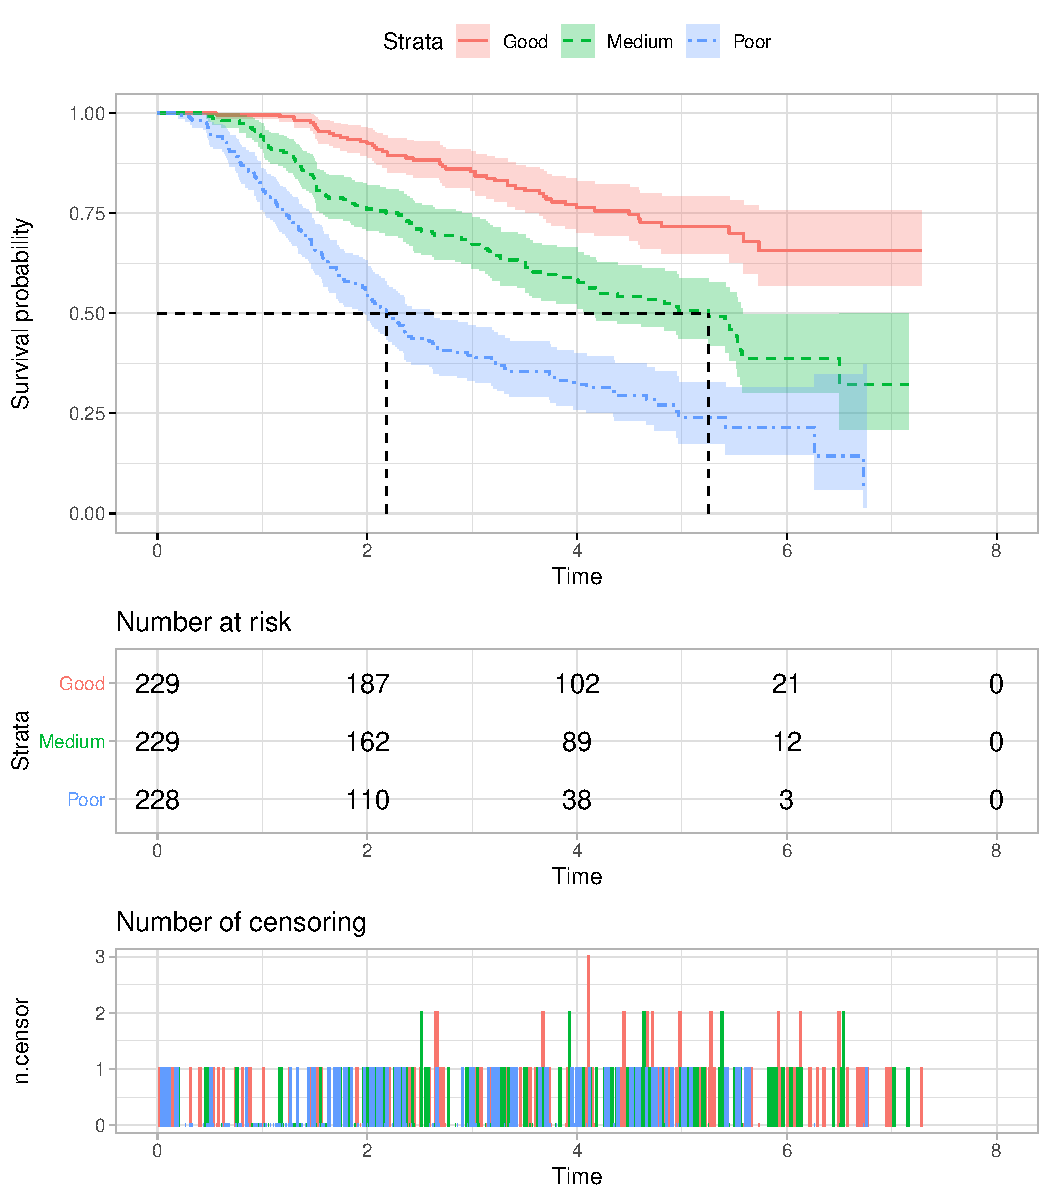
\includegraphics{Images/plot_KM-1} \end{flushleft}

\begin{table}[H]
\centering
\begin{tabular}{lrrrrrrrrr}
\toprule
  & records & n.max & n.start & events & *rmean & *se(rmean) & median & 0.95LCL & 0.95UCL\\
\midrule
\cellcolor{gray!6}{group=Good} & \cellcolor{gray!6}{229} & \cellcolor{gray!6}{229} & \cellcolor{gray!6}{229} & \cellcolor{gray!6}{51} & \cellcolor{gray!6}{5.934330} & \cellcolor{gray!6}{0.1616003} & \cellcolor{gray!6}{NA} & \cellcolor{gray!6}{NA} & \cellcolor{gray!6}{NA}\\
group=Medium & 229 & 229 & 229 & 103 & 4.600852 & 0.1856699 & 5.254795 & 4.115068 & 5.572603\\
\cellcolor{gray!6}{group=Poor} & \cellcolor{gray!6}{228} & \cellcolor{gray!6}{228} & \cellcolor{gray!6}{228} & \cellcolor{gray!6}{145} & \cellcolor{gray!6}{3.101736} & \cellcolor{gray!6}{0.1772520} & \cellcolor{gray!6}{2.183562} & \cellcolor{gray!6}{1.978082} & \cellcolor{gray!6}{2.619178}\\
\bottomrule
\end{tabular}
\end{table}

\newpage

\section{Stratified models?}\label{stratified-models}

Should stratified parametric survival models be used?

\begin{flushleft}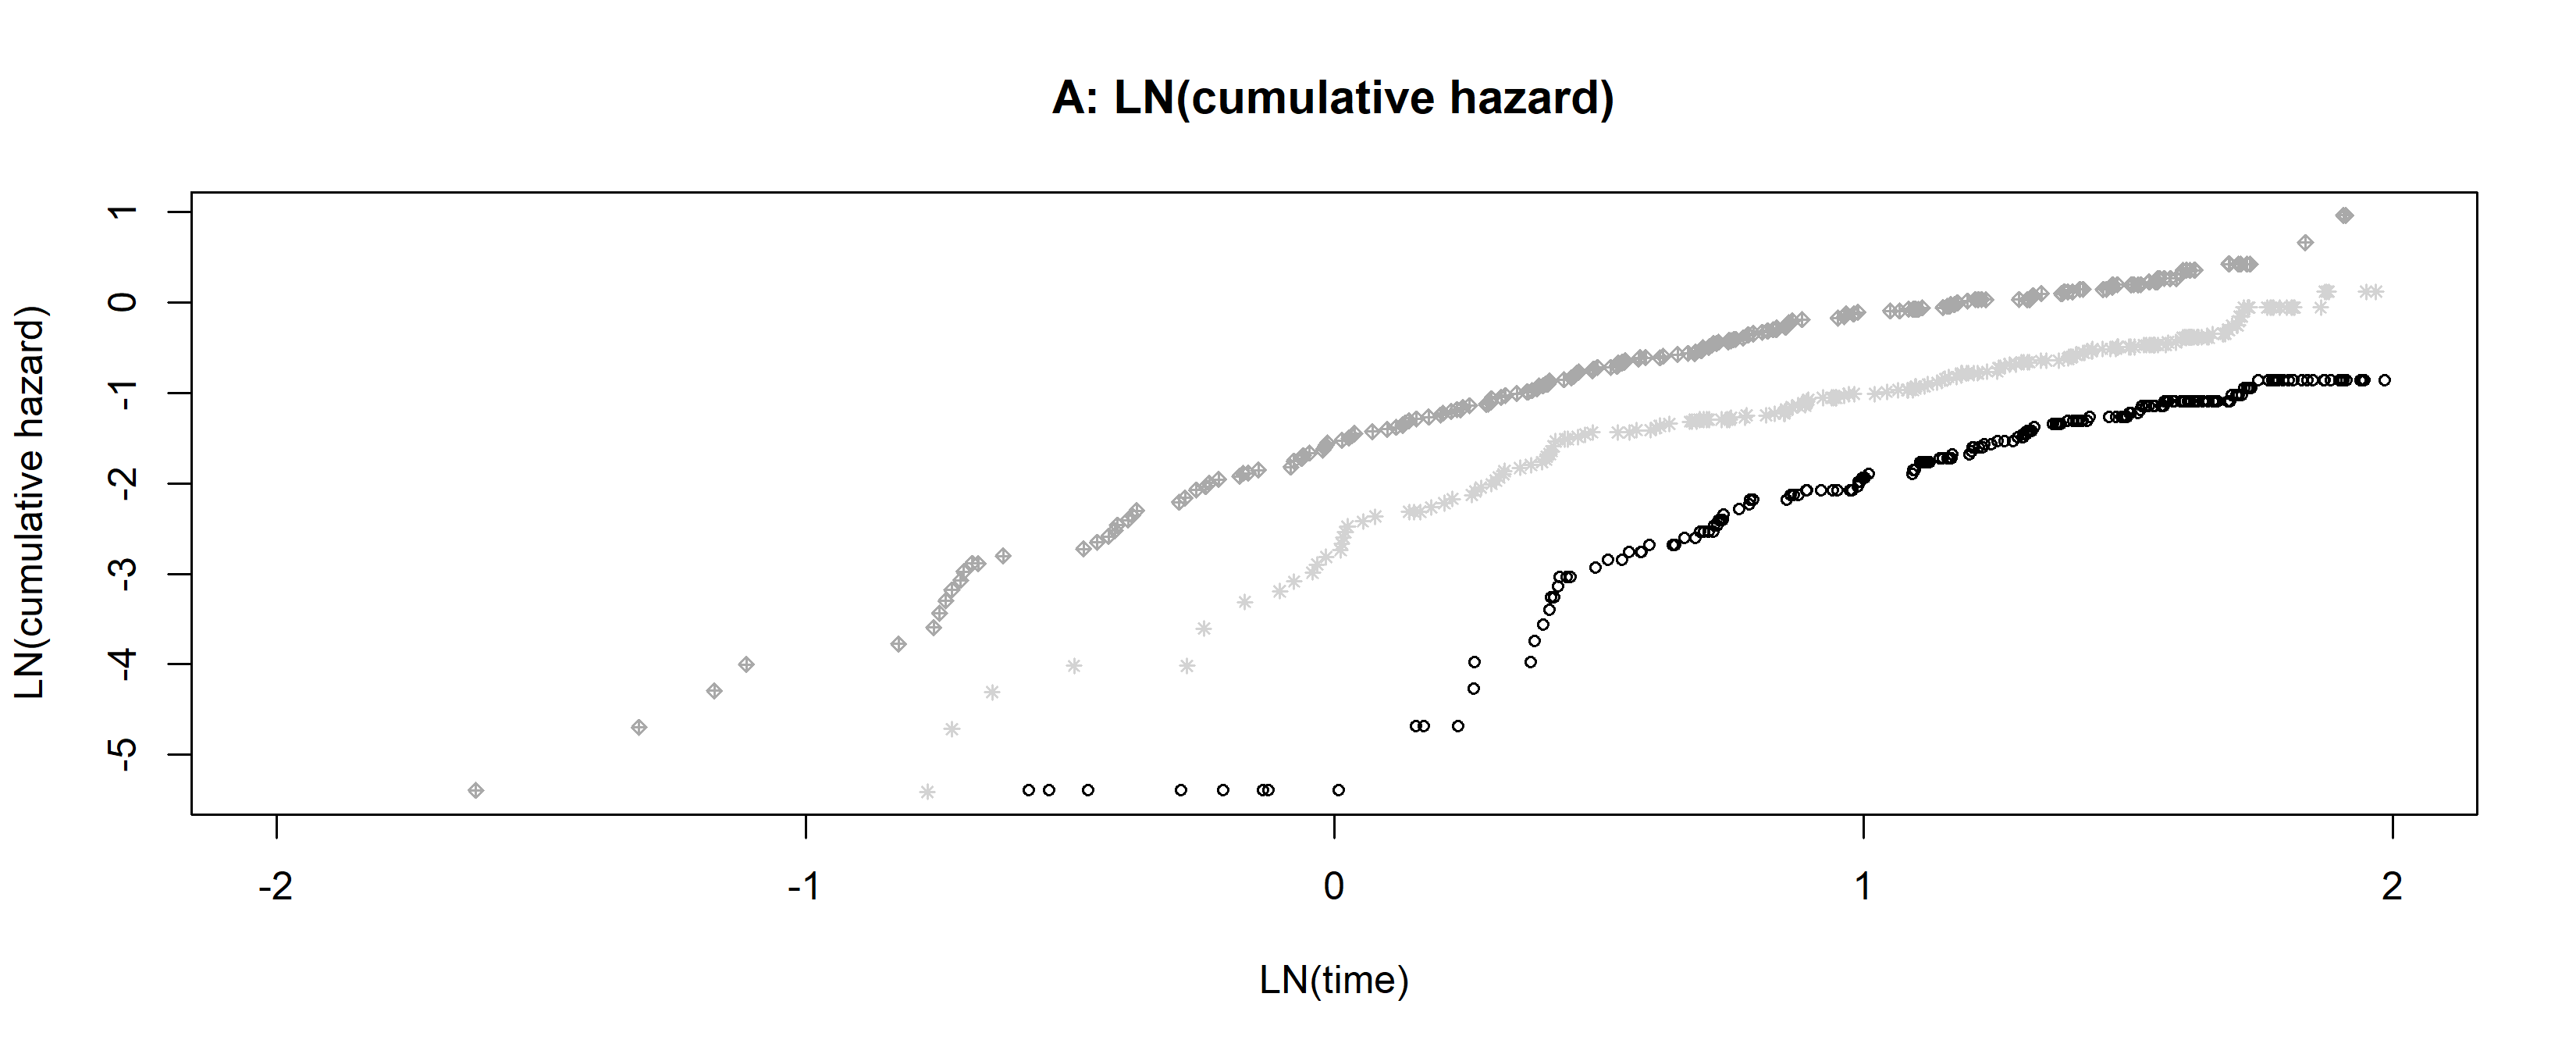
\includegraphics[height=0.29\textheight]{Images/PH_assumption-1} \end{flushleft}

\begin{flushleft}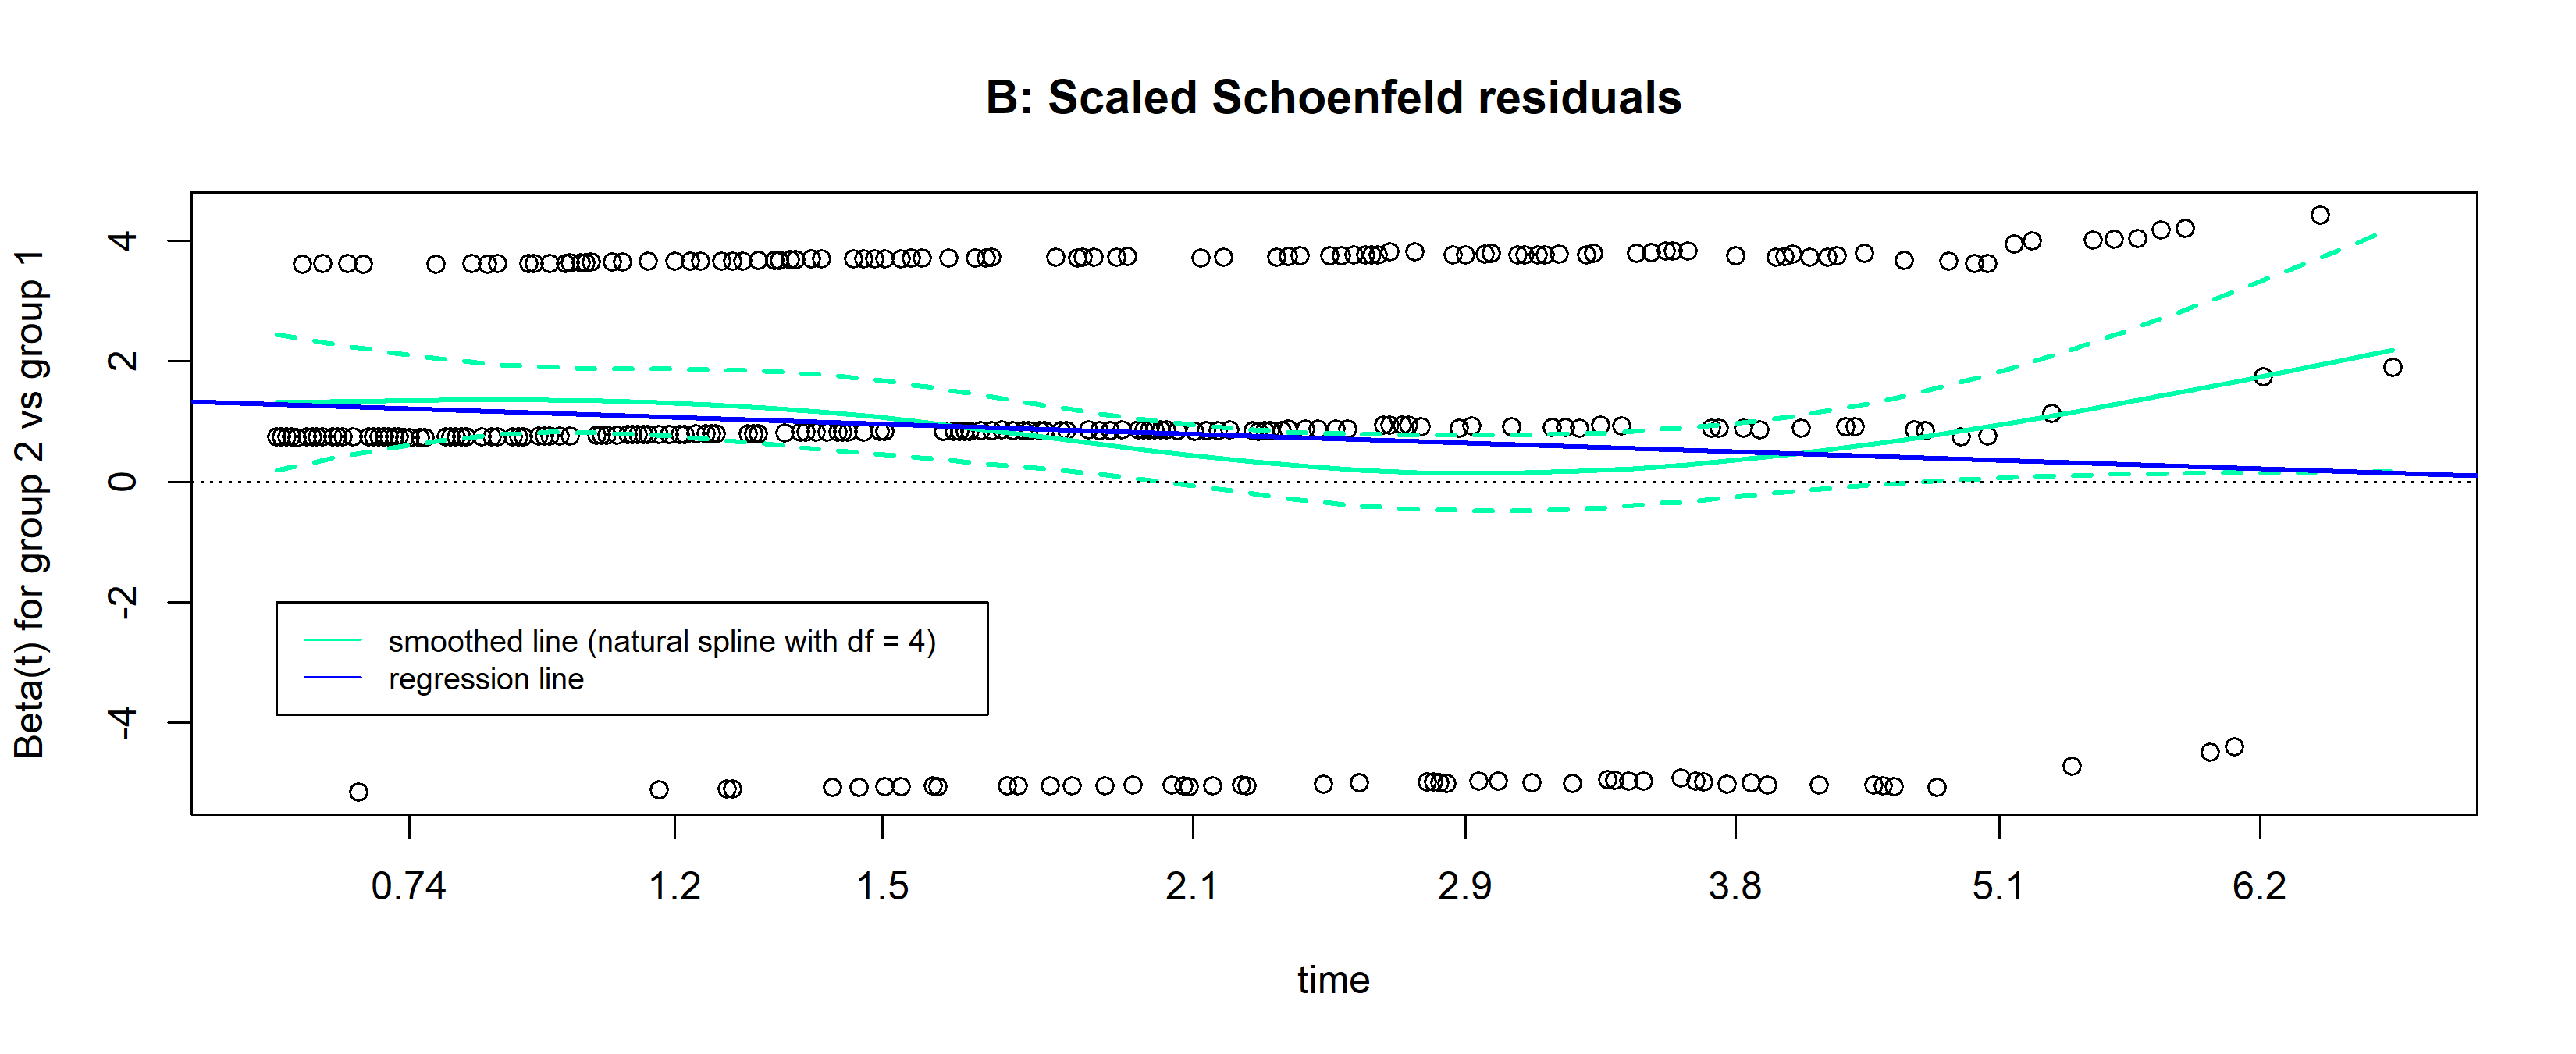
\includegraphics[height=0.29\textheight]{Images/PH_assumption-2} \end{flushleft}

\begin{flushleft}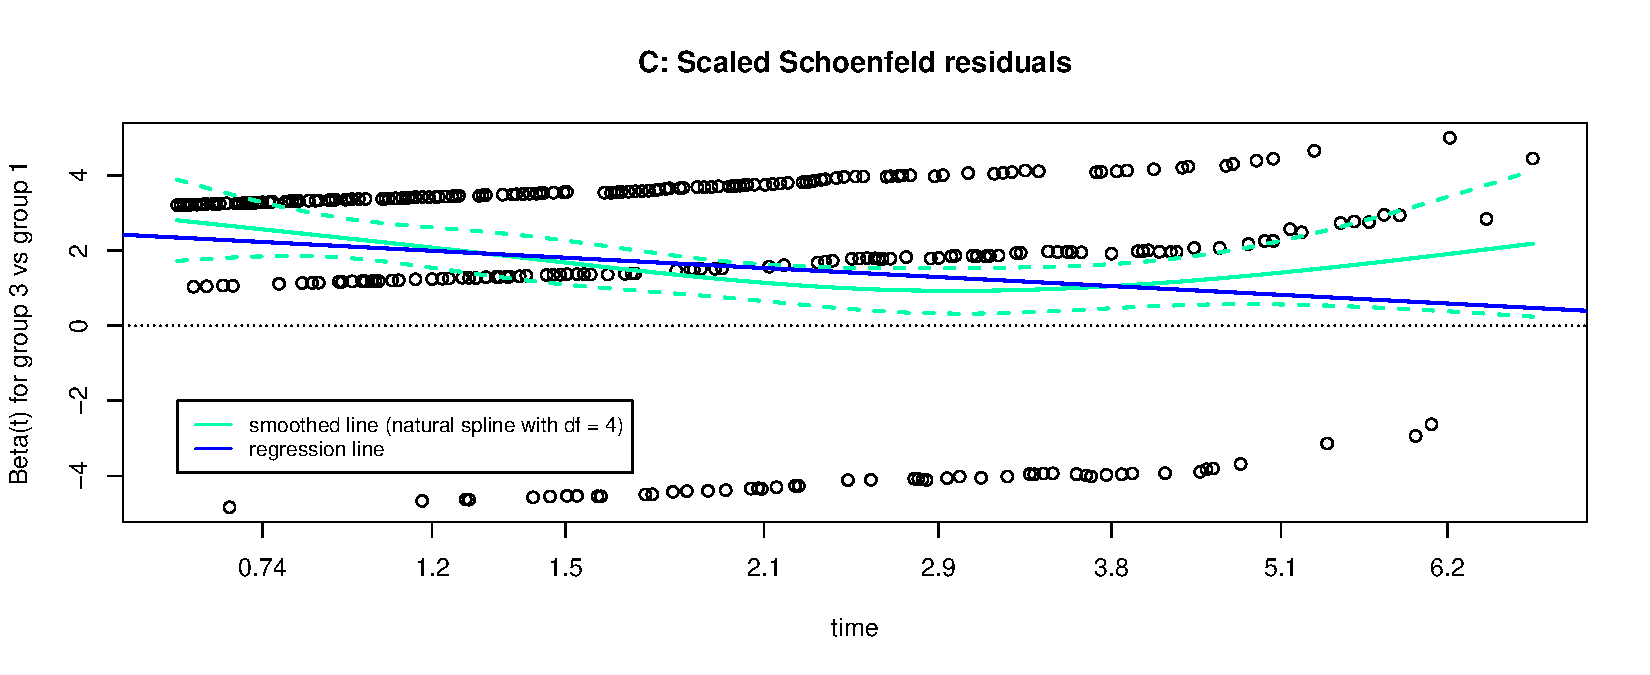
\includegraphics[height=0.29\textheight]{Images/PH_assumption-3} \end{flushleft}

\newpage

\section{Shape of the observed smoothed hazard
function}\label{shape-of-the-observed-smoothed-hazard-function}

Should parametric survival models assuming a monotonic hazard rate
(i.e.~exponential, Weibull, Gompertz) be used?

\begin{flushleft}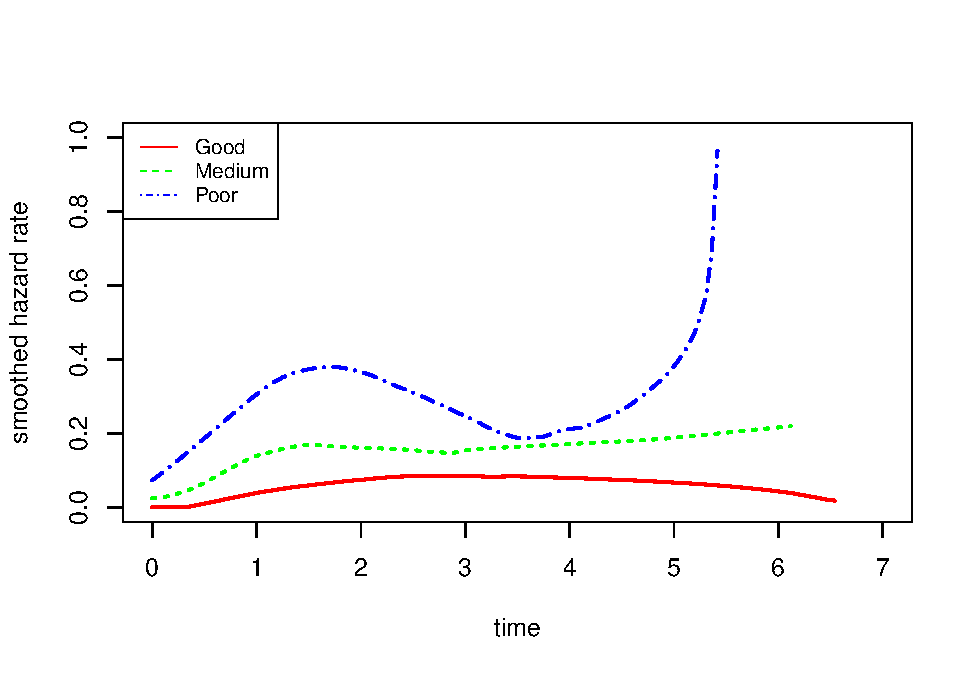
\includegraphics{Images/plot_hr-1} \end{flushleft}

\newpage

\section{Shape of the predicted hazard
function}\label{shape-of-the-predicted-hazard-function}

\begin{flushleft}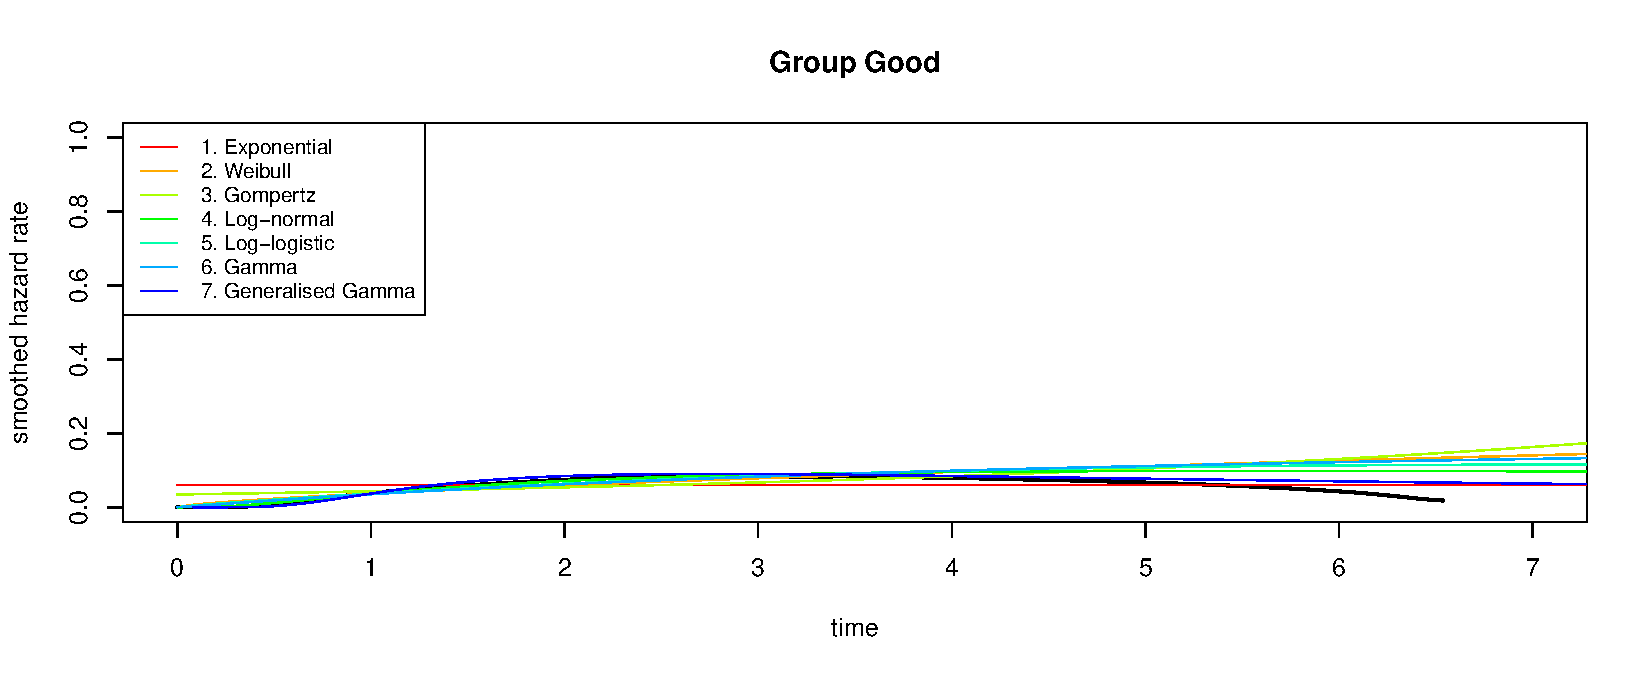
\includegraphics[height=0.29\textheight]{Images/plot_haz_pred-1} \end{flushleft}

\begin{flushleft}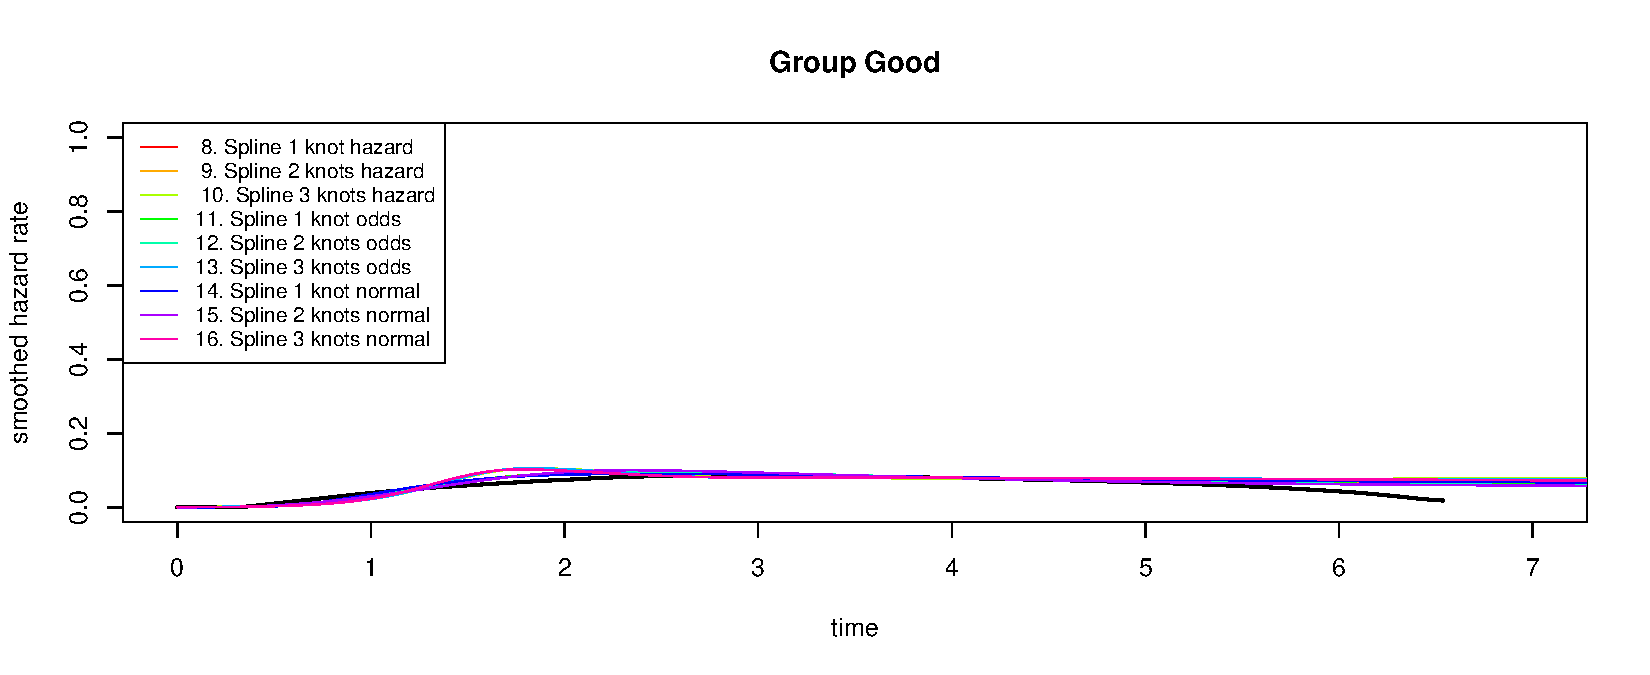
\includegraphics[height=0.29\textheight]{Images/plot_haz_pred-2} \end{flushleft}

\begin{flushleft}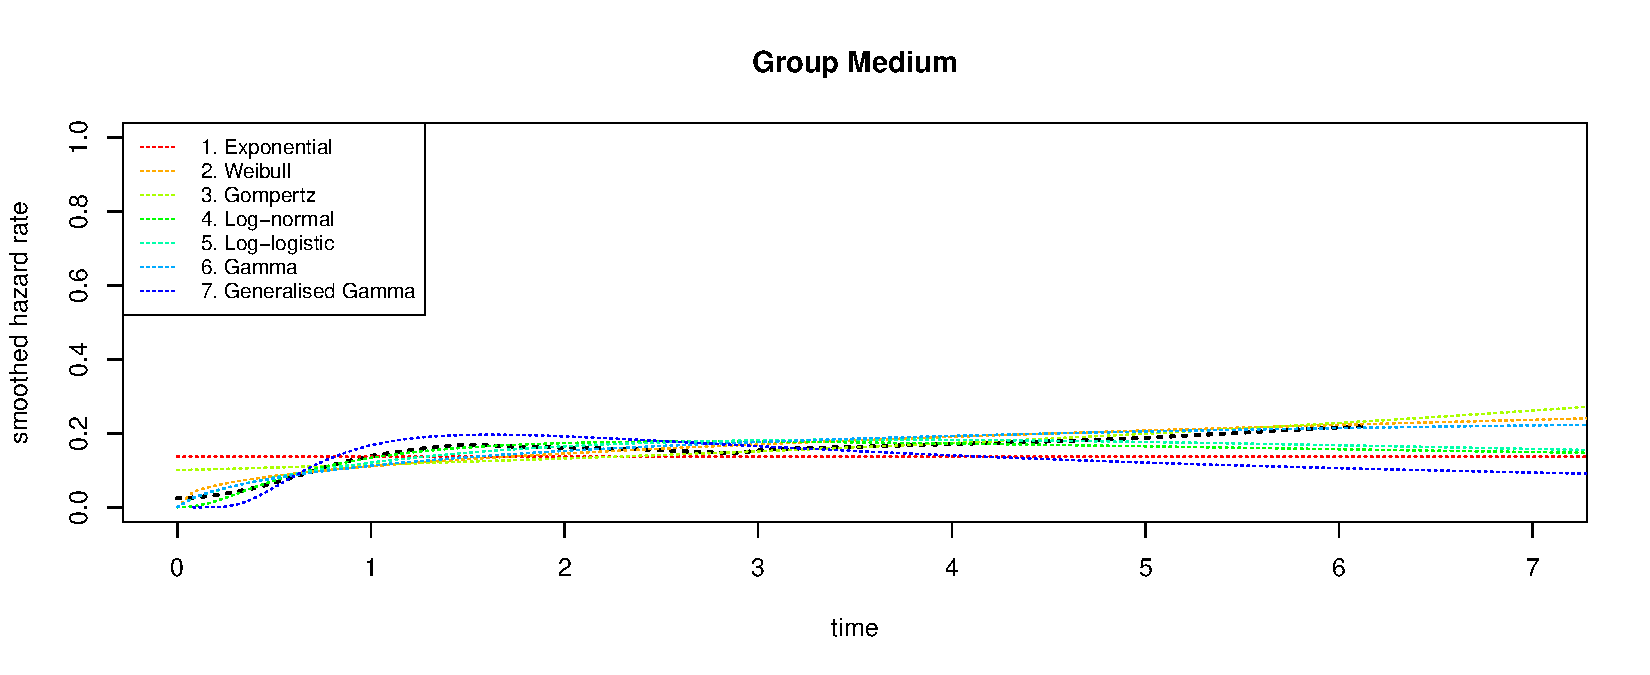
\includegraphics[height=0.29\textheight]{Images/plot_haz_pred-3} \end{flushleft}

\begin{flushleft}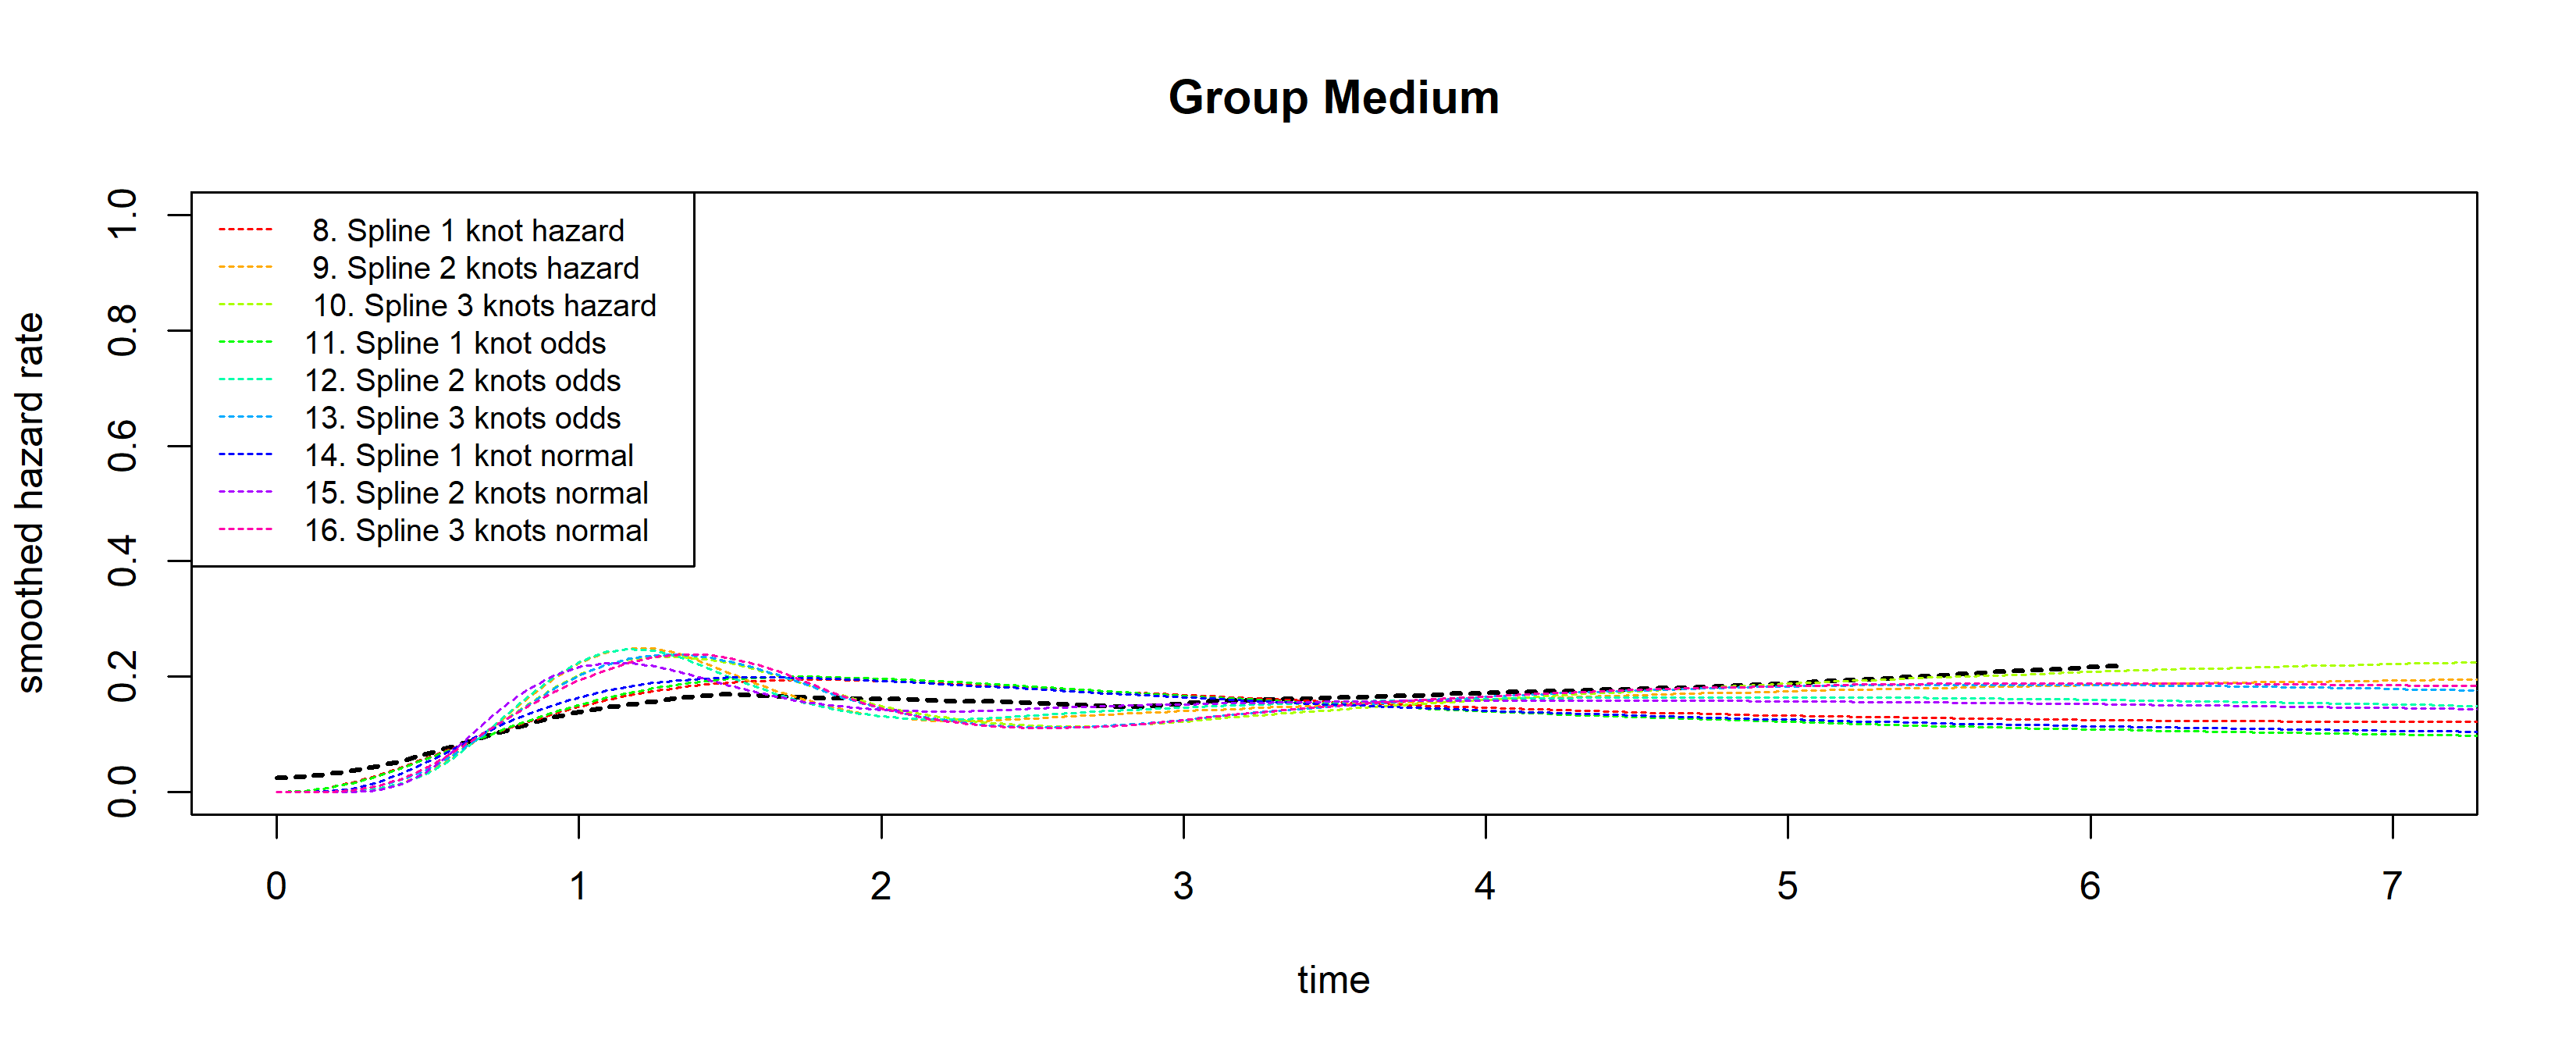
\includegraphics[height=0.29\textheight]{Images/plot_haz_pred-4} \end{flushleft}

\begin{flushleft}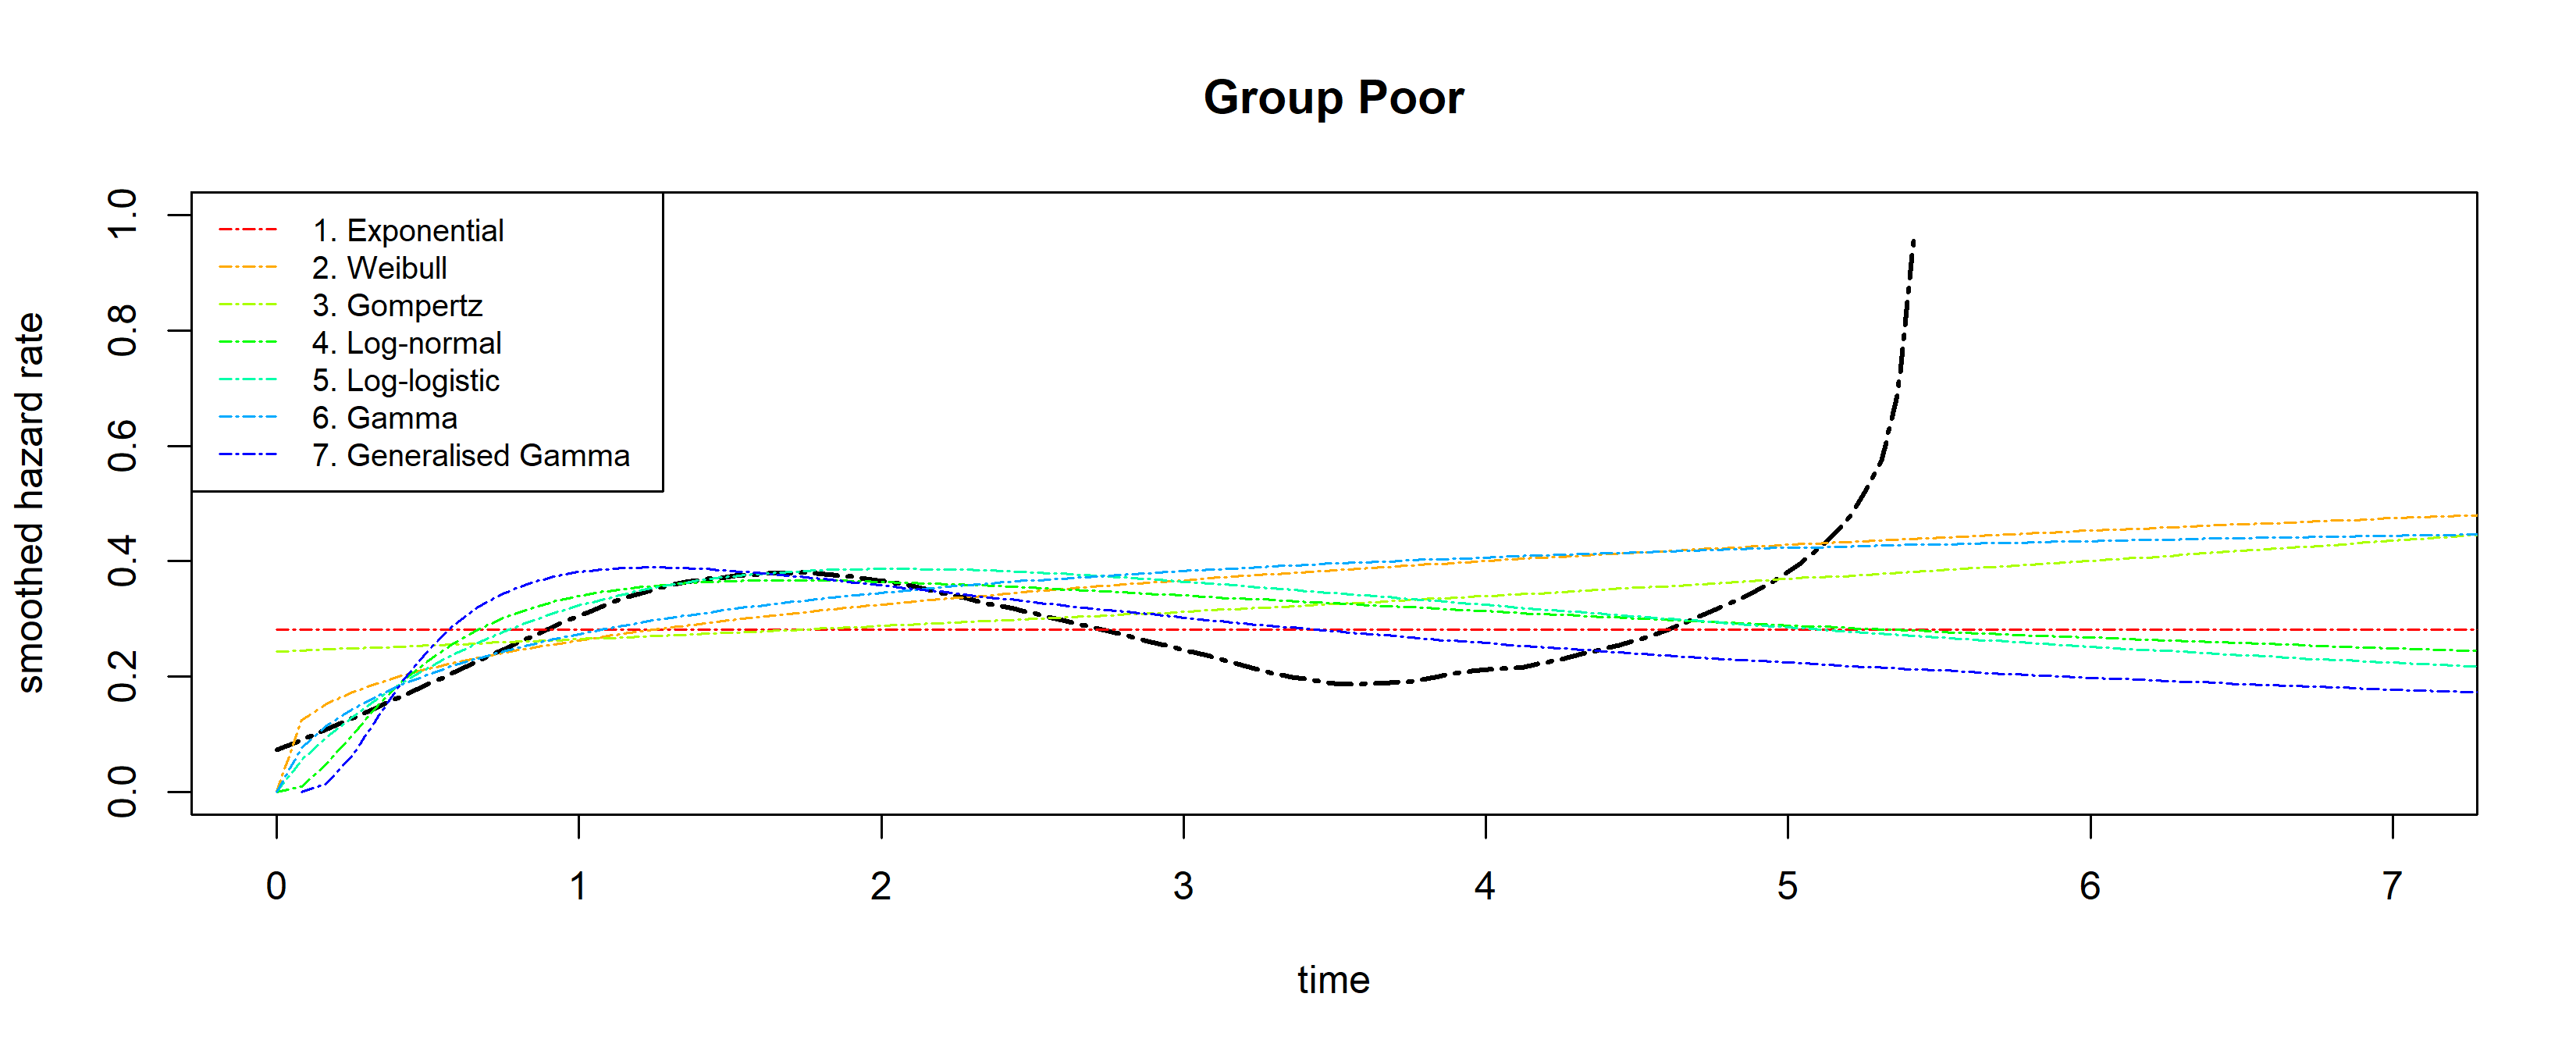
\includegraphics[height=0.29\textheight]{Images/plot_haz_pred-5} \end{flushleft}

\begin{flushleft}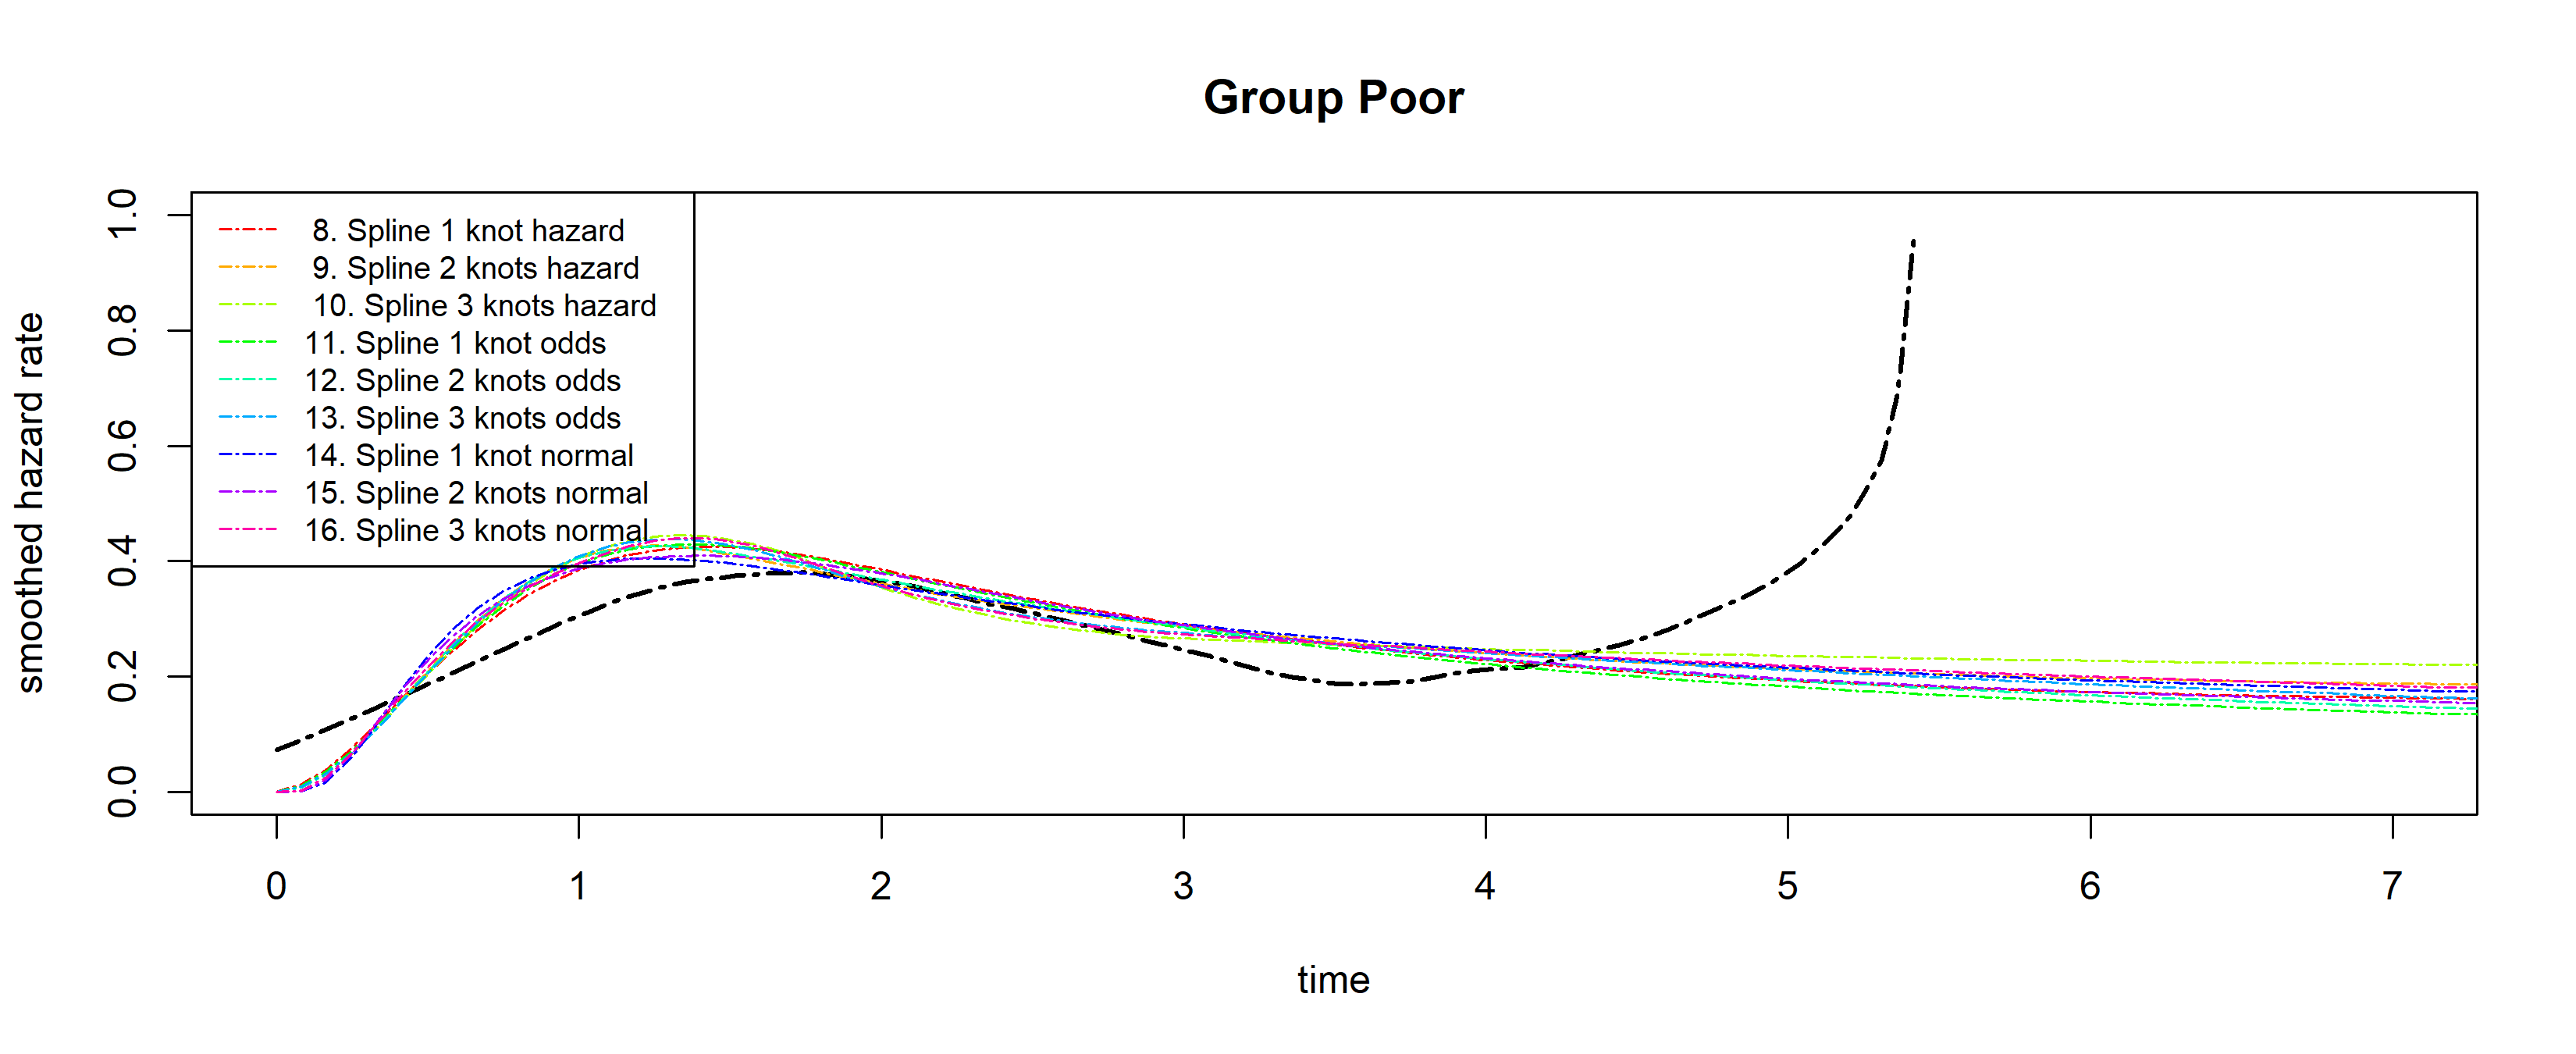
\includegraphics[height=0.29\textheight]{Images/plot_haz_pred-6} \end{flushleft}

\newpage

\section{Standard parametric models?}\label{standard-parametric-models}

Do standard parametric models provide an appropriate fit to the data?

\begin{flushleft}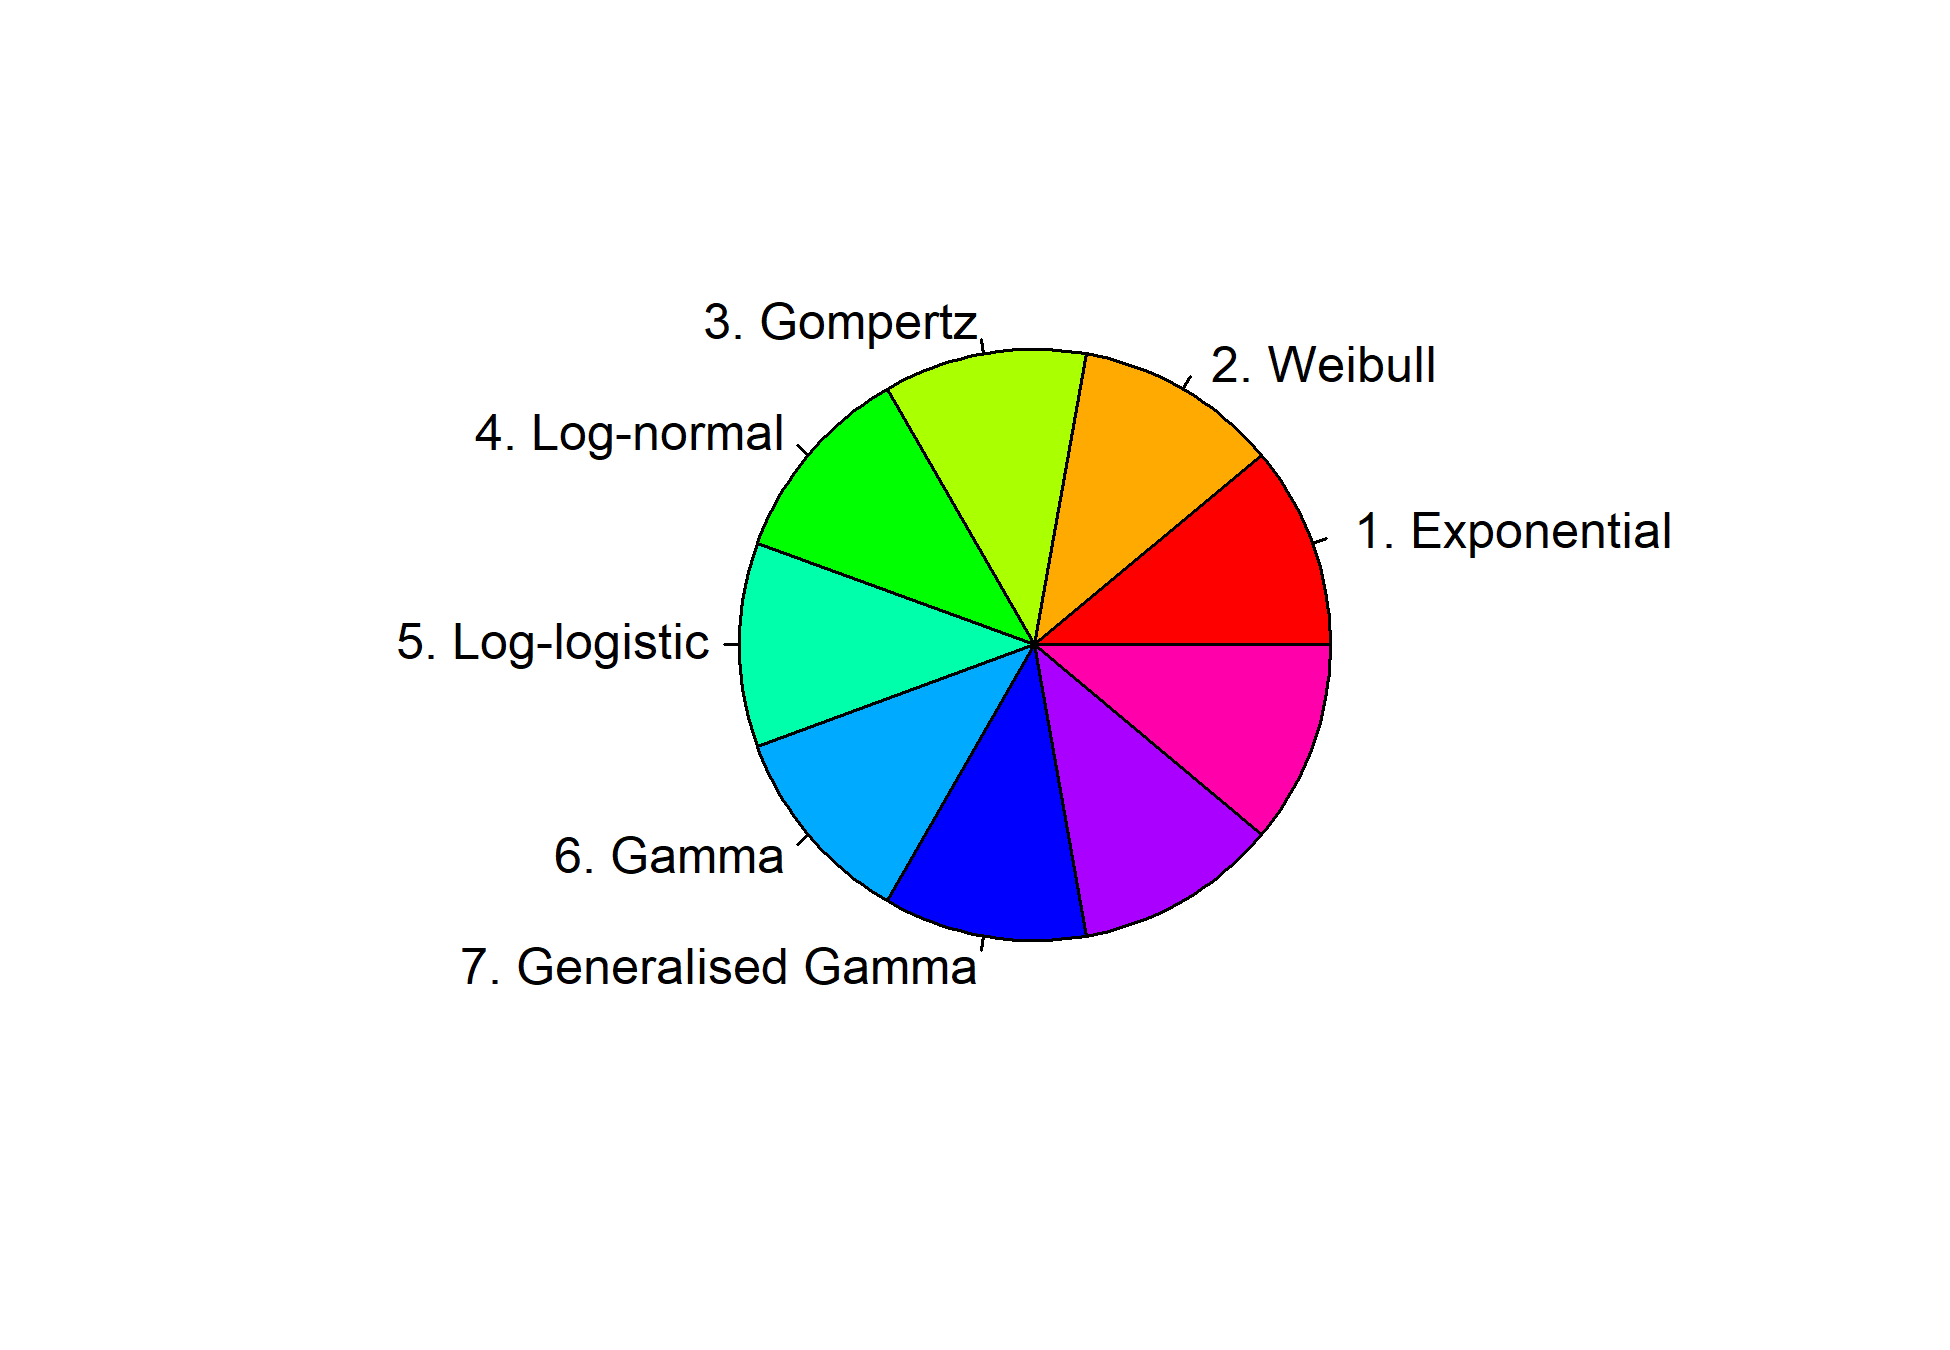
\includegraphics{Images/plot_parametric-1} \end{flushleft}

\begin{table}[H]
\centering
\begin{tabular}{lrr}
\toprule
Model & AIC & BIC\\
\midrule
\cellcolor{gray!6}{7. Generalised Gamma} & \cellcolor{gray!6}{1589.049} & \cellcolor{gray!6}{1629.826}\\
4. Log-normal & 1592.880 & 1620.066\\
\cellcolor{gray!6}{5. Log-logistic} & \cellcolor{gray!6}{1609.294} & \cellcolor{gray!6}{1636.479}\\
6. Gamma & 1621.982 & 1649.167\\
\cellcolor{gray!6}{2. Weibull} & \cellcolor{gray!6}{1632.618} & \cellcolor{gray!6}{1659.803}\\
3. Gompertz & 1660.954 & 1688.140\\
\cellcolor{gray!6}{1. Exponential} & \cellcolor{gray!6}{1668.212} & \cellcolor{gray!6}{1681.805}\\
\bottomrule
\end{tabular}
\end{table}

\subsection{Exponential}\label{exponential}

\begin{flushleft}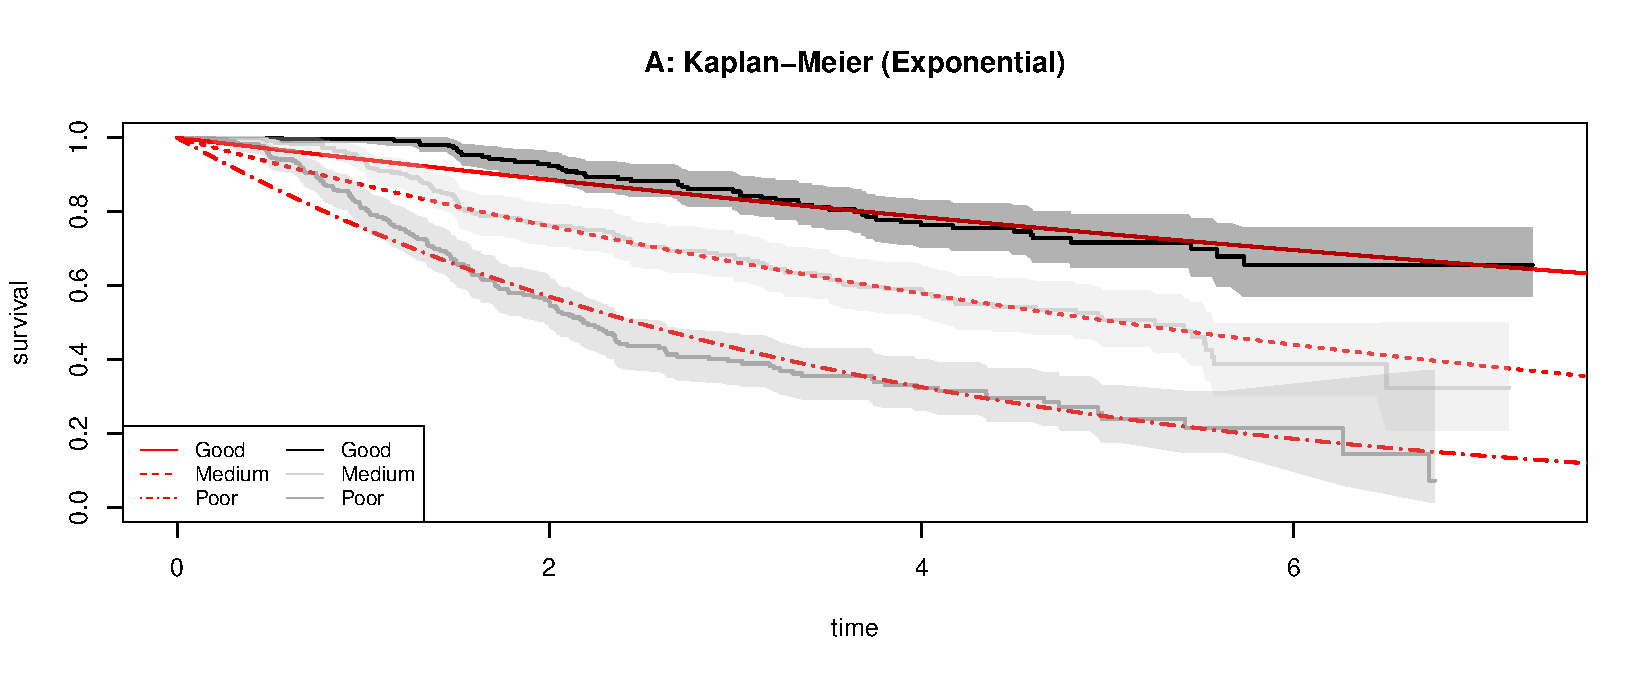
\includegraphics[height=0.3\textheight]{Images/expo-1} \end{flushleft}

\begin{flushleft}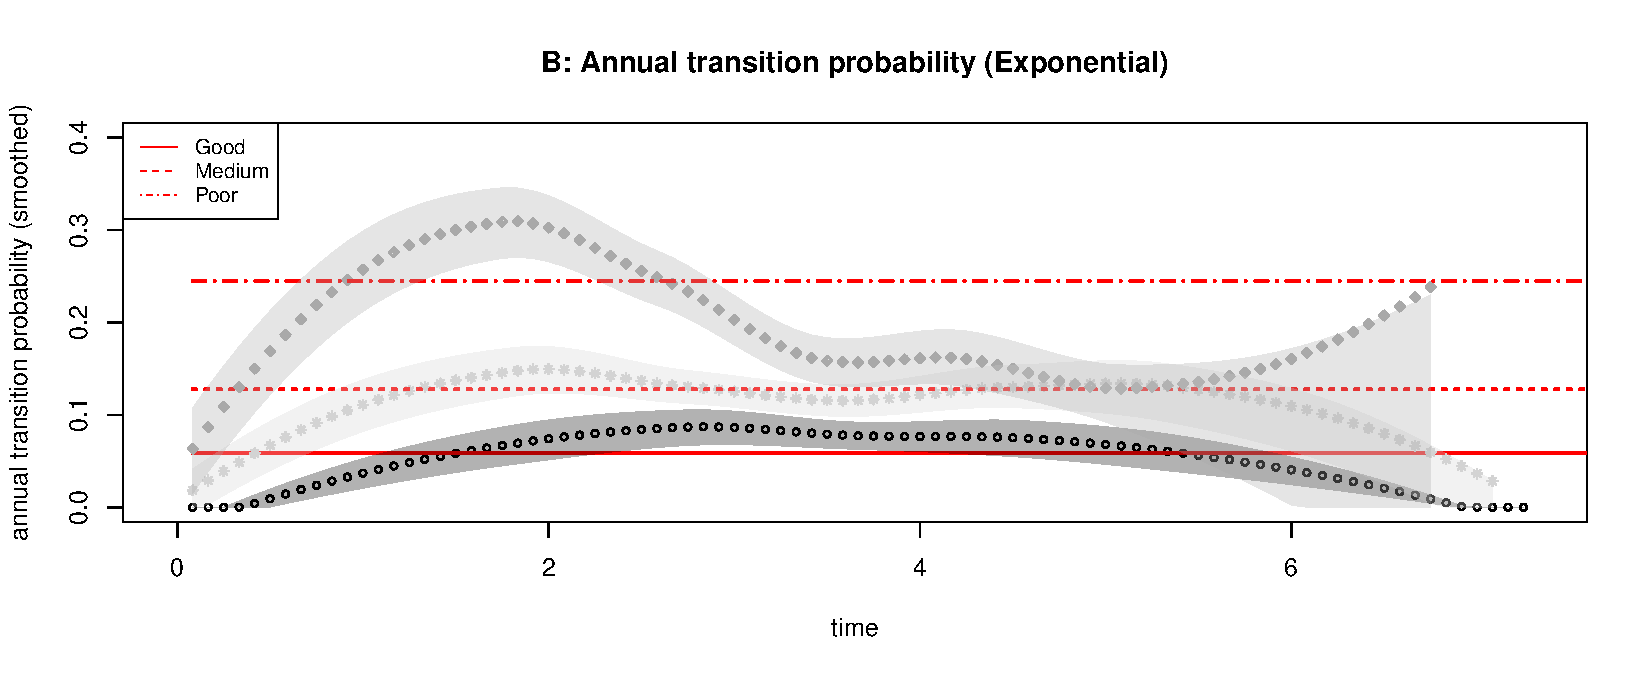
\includegraphics[height=0.3\textheight]{Images/expo-2} \end{flushleft}

\begin{flushleft}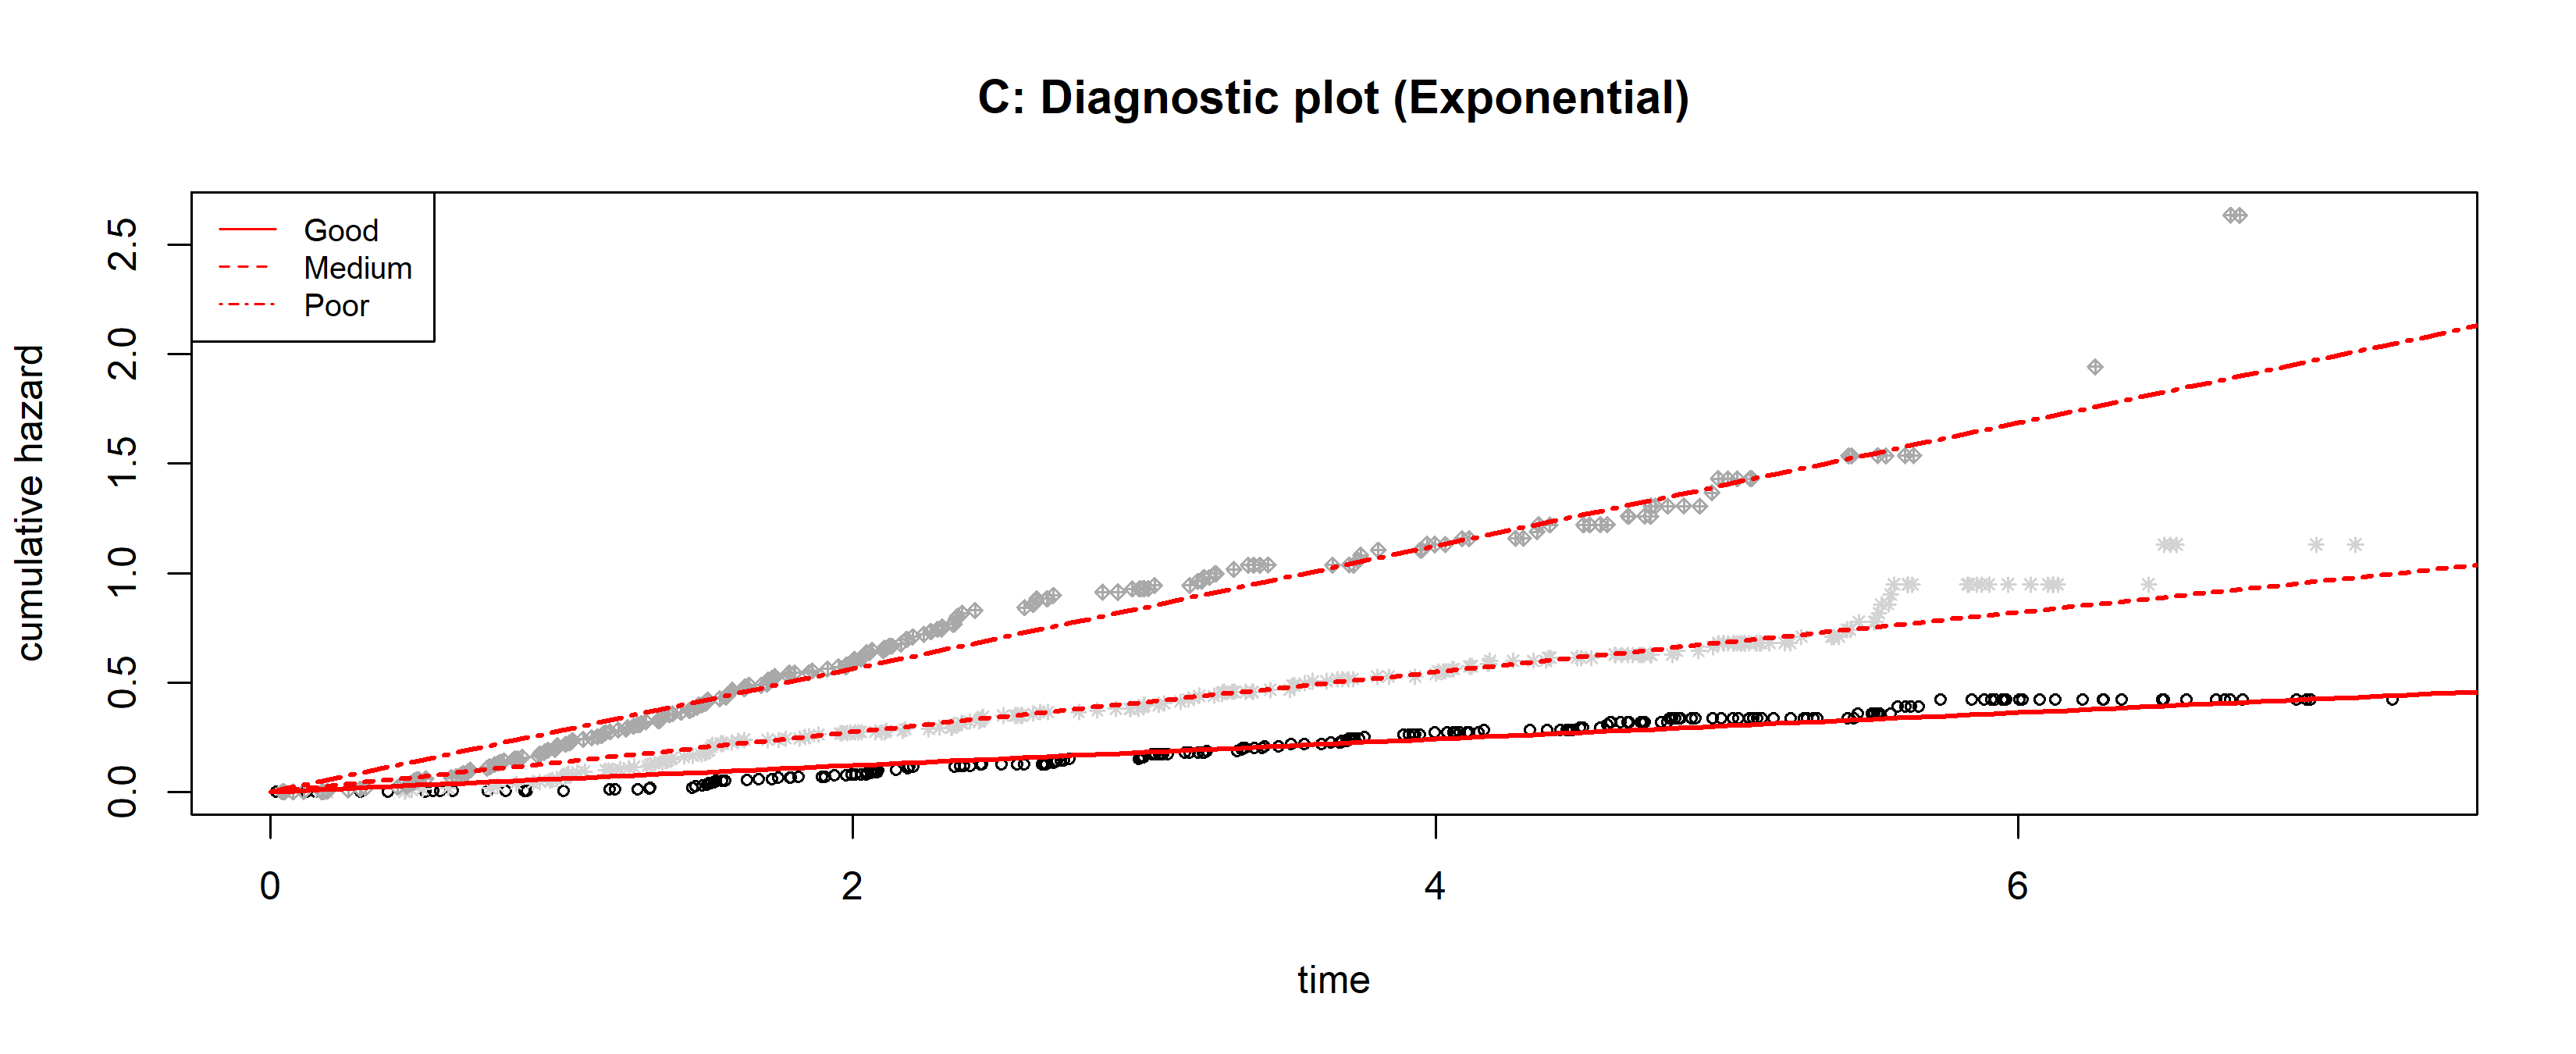
\includegraphics[height=0.3\textheight]{Images/expo-3} \end{flushleft}

\subsection{Weibull}\label{weibull}

\begin{flushleft}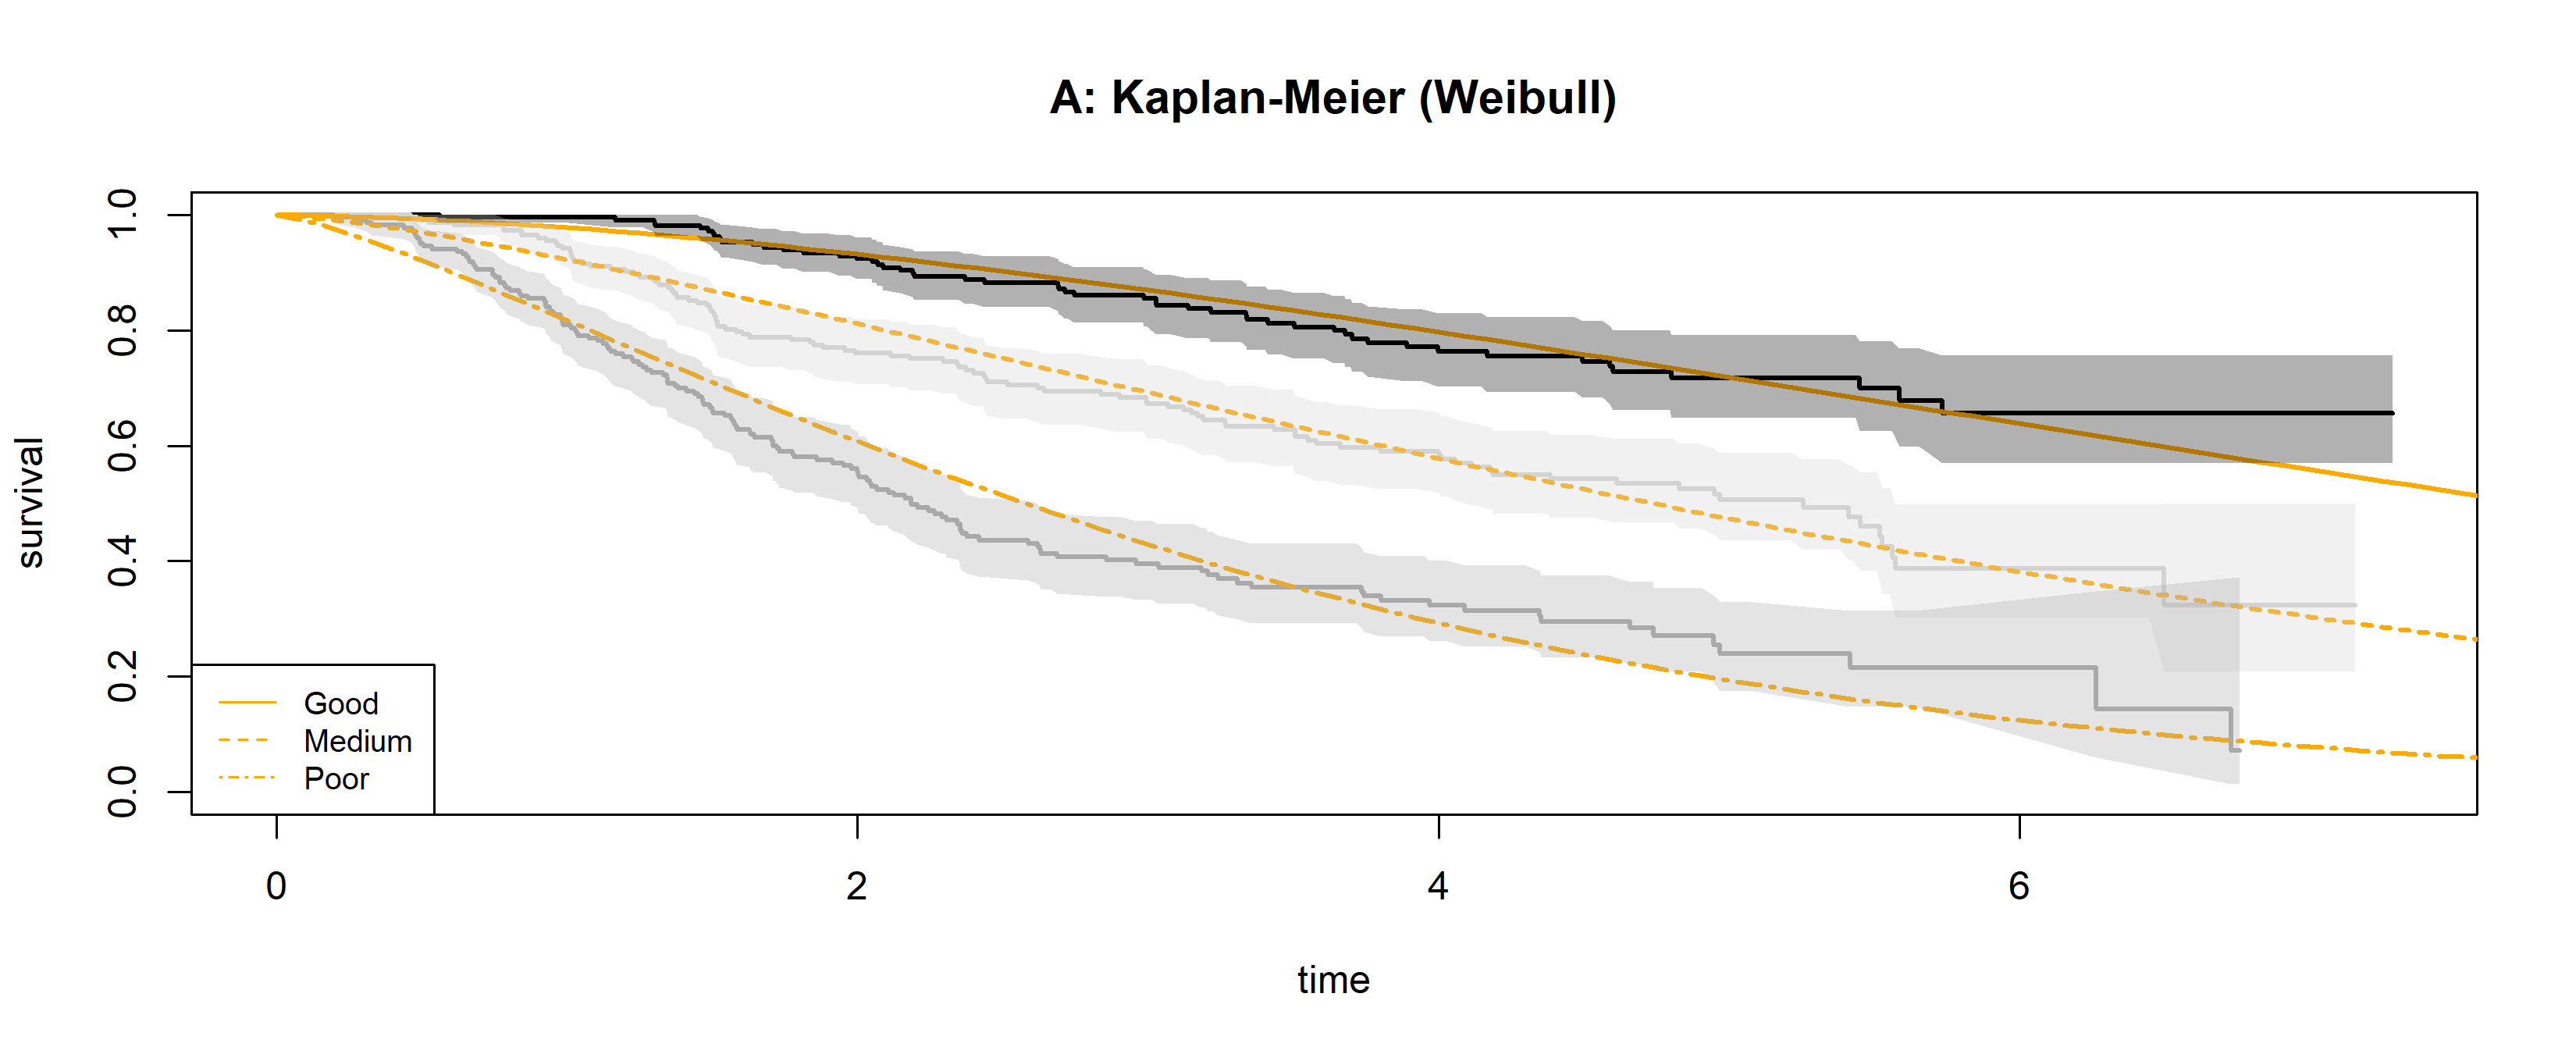
\includegraphics[height=0.3\textheight]{Images/weib-1} \end{flushleft}

\begin{flushleft}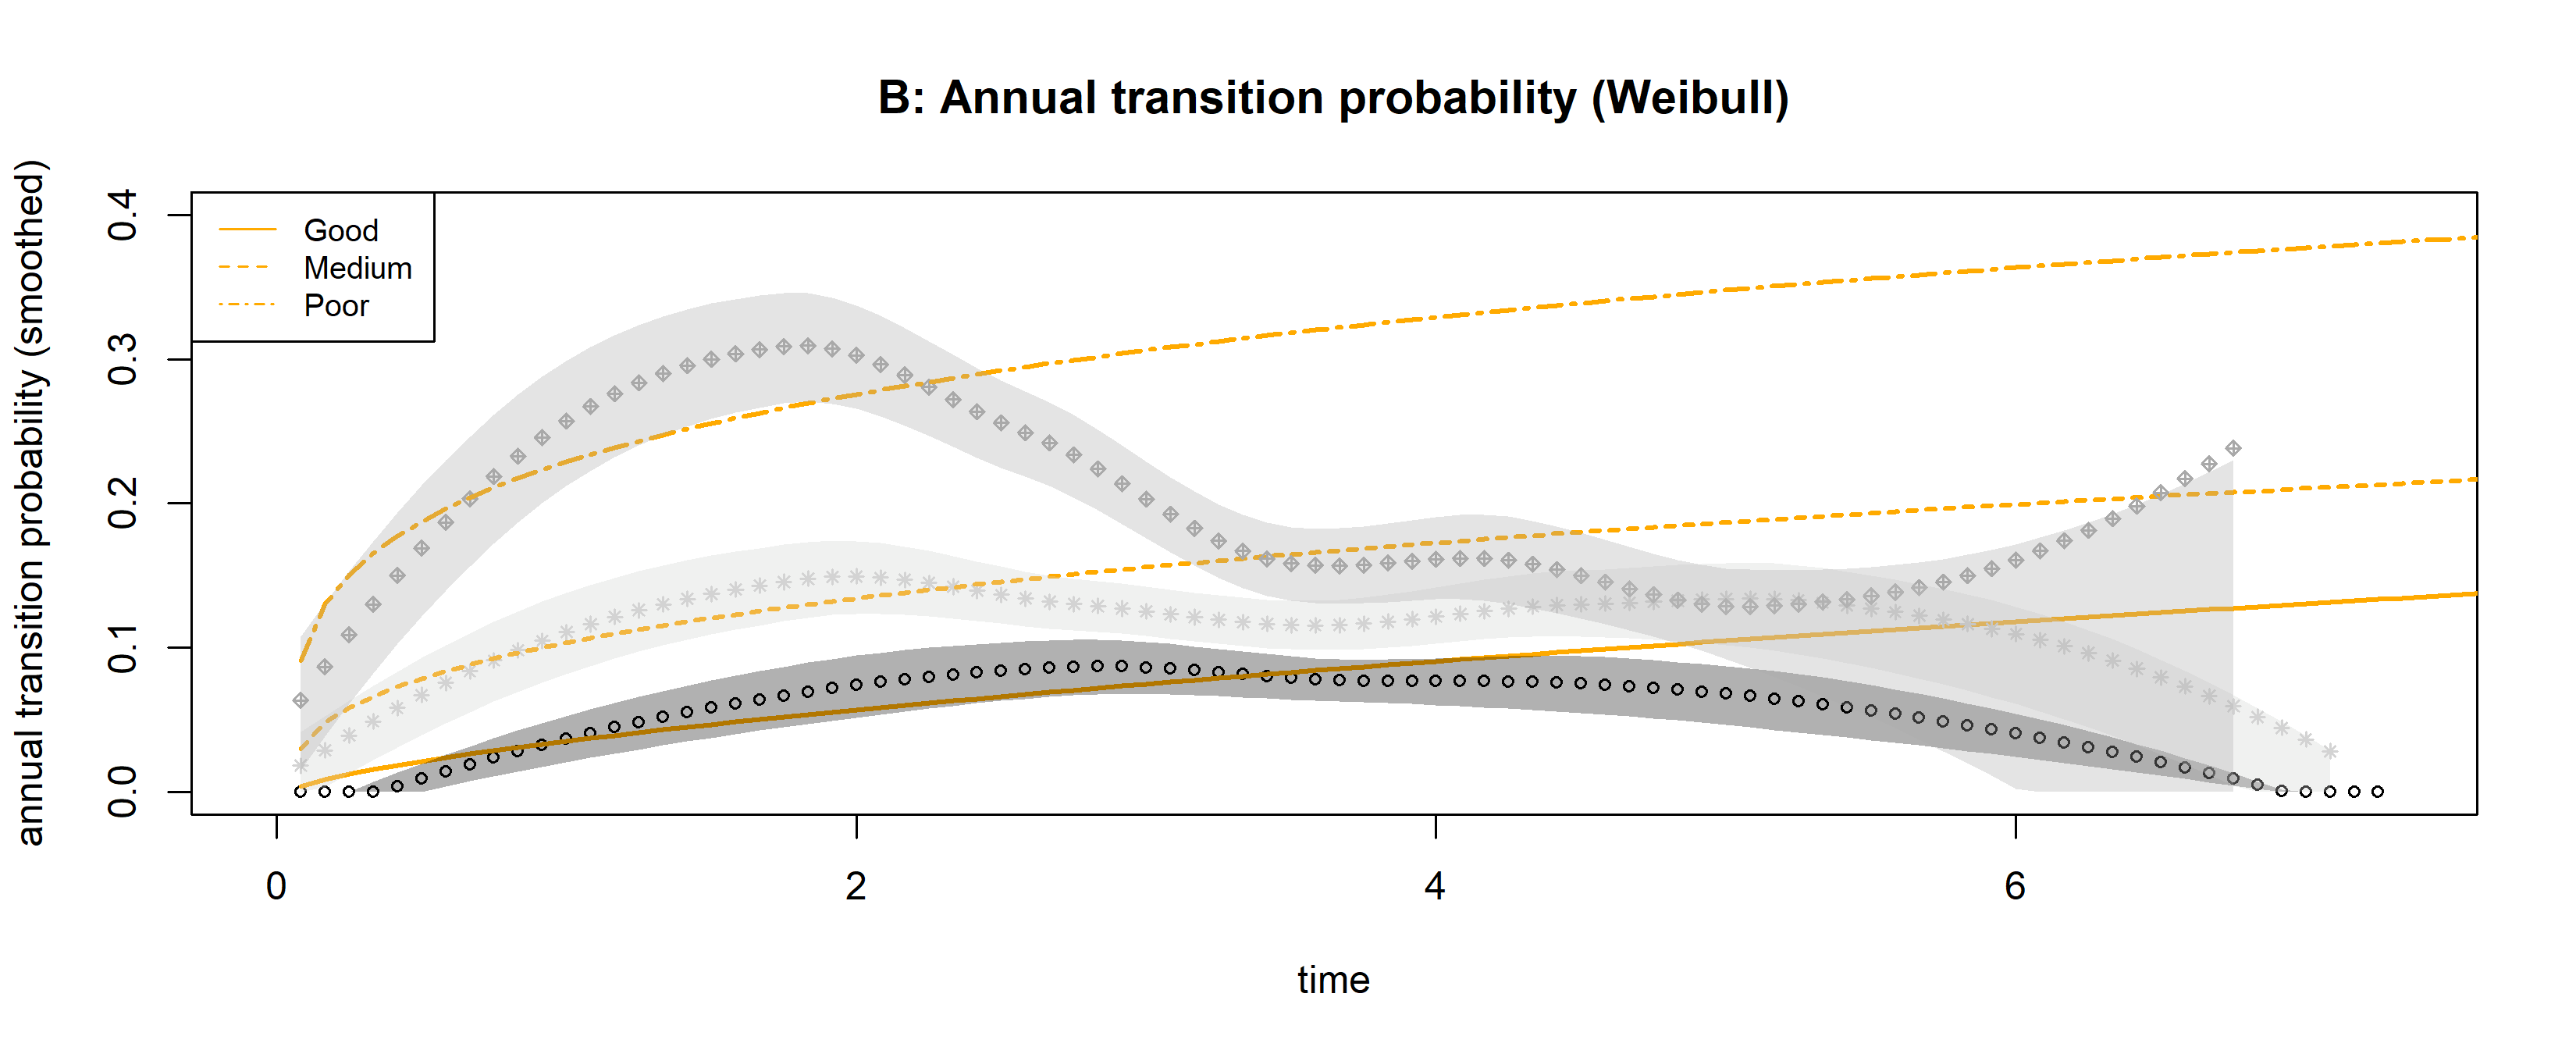
\includegraphics[height=0.3\textheight]{Images/weib-2} \end{flushleft}

\begin{flushleft}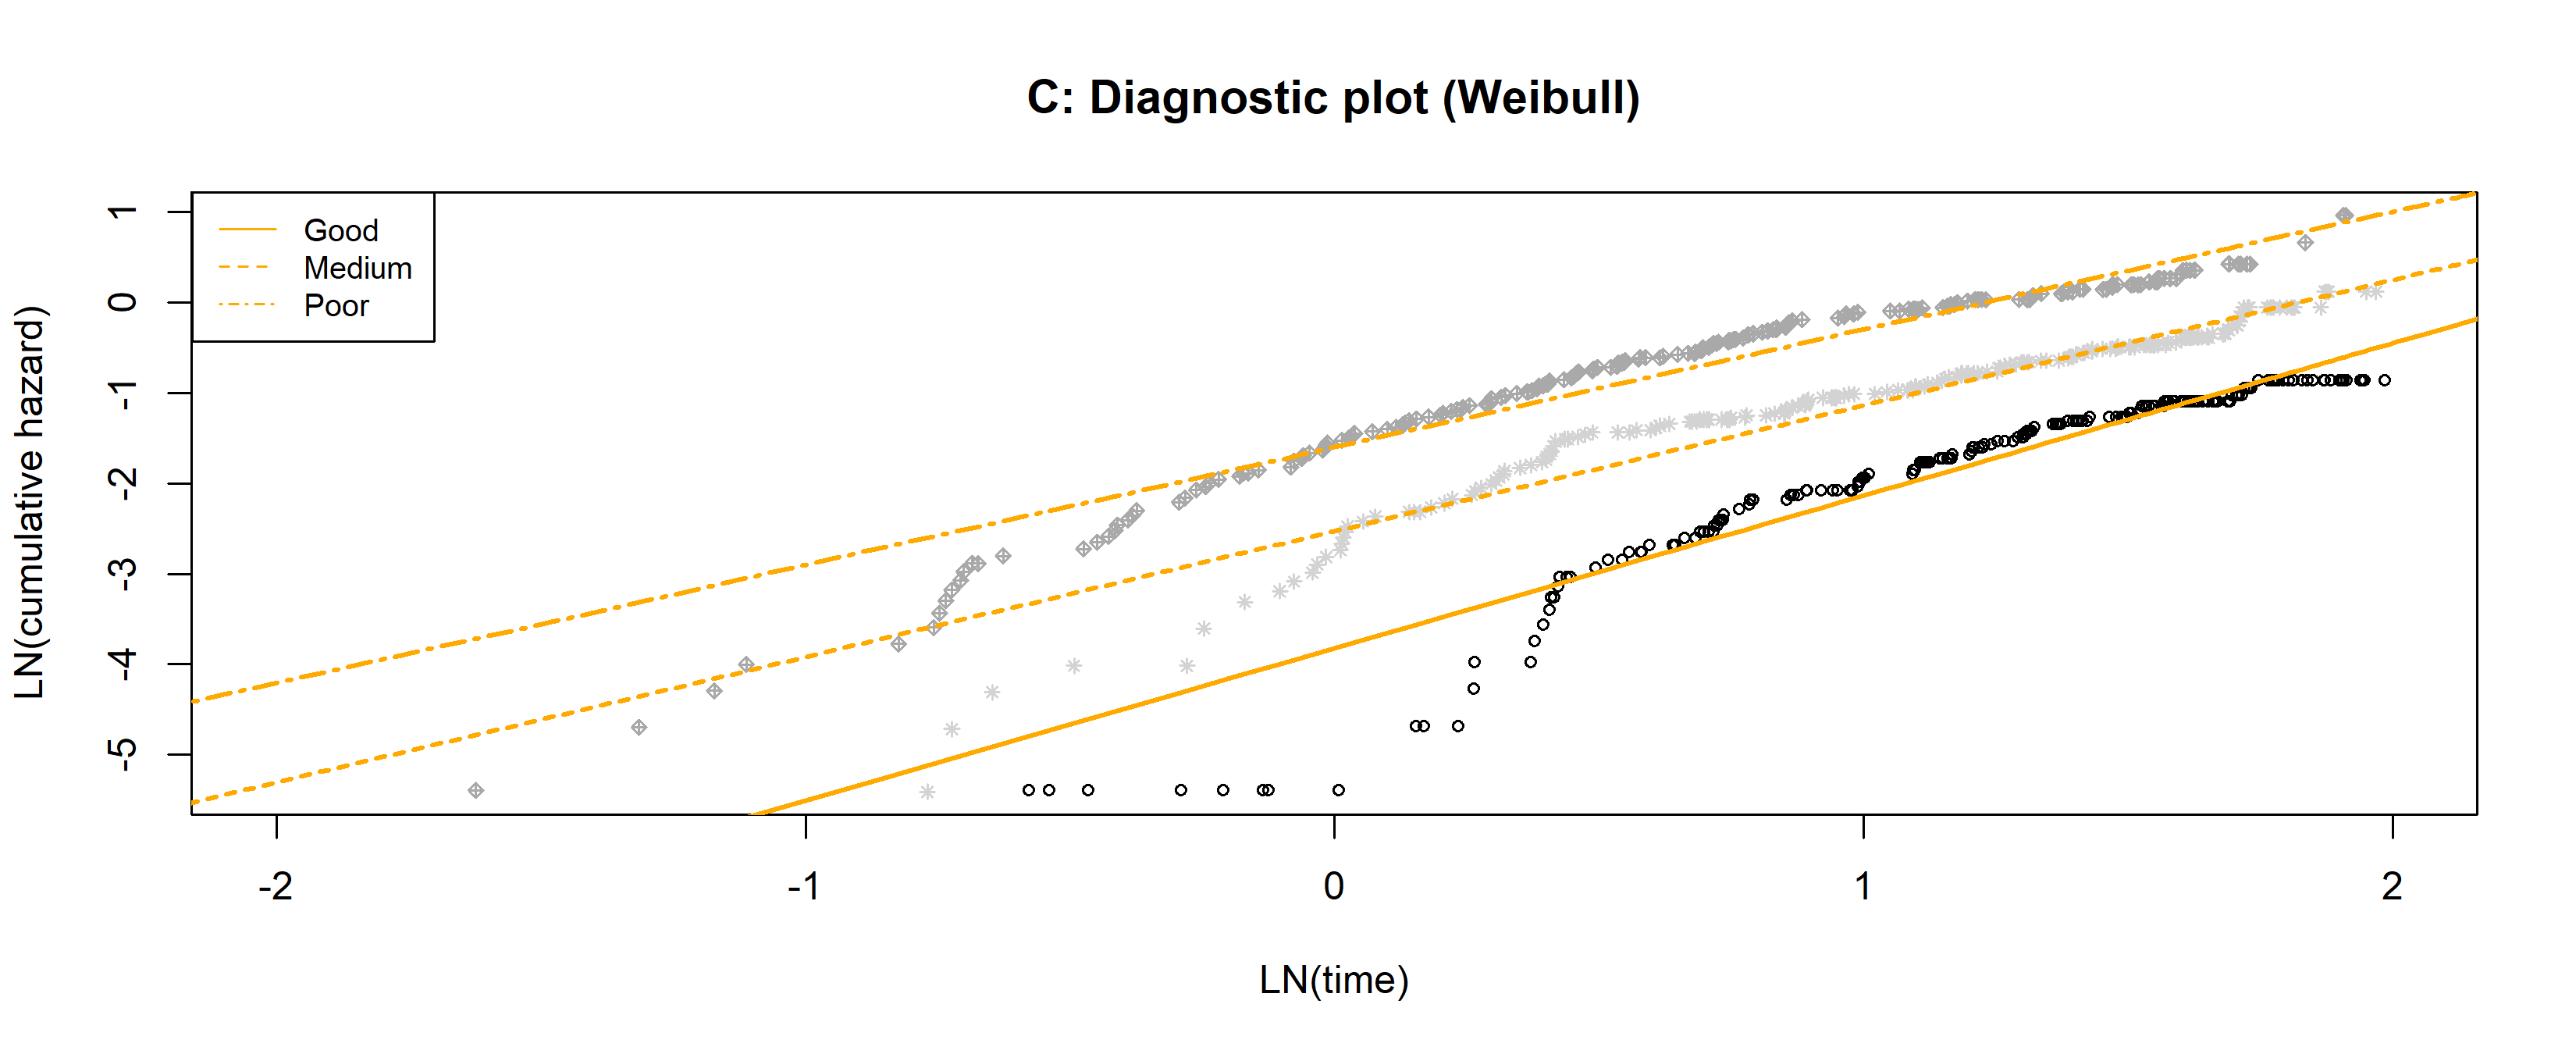
\includegraphics[height=0.3\textheight]{Images/weib-3} \end{flushleft}

\subsection{Gompertz}\label{gompertz}

\begin{flushleft}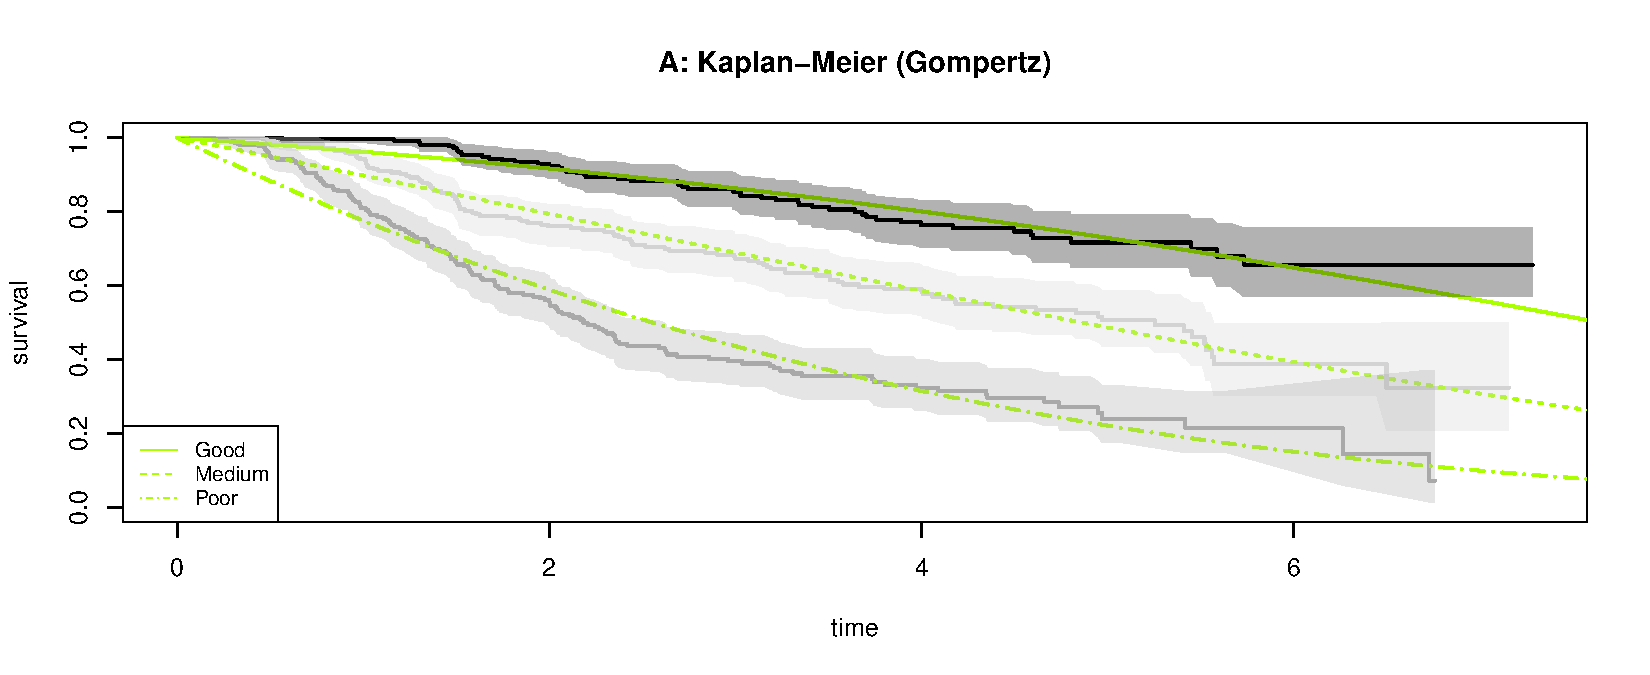
\includegraphics[height=0.3\textheight]{Images/gom-1} \end{flushleft}

\begin{flushleft}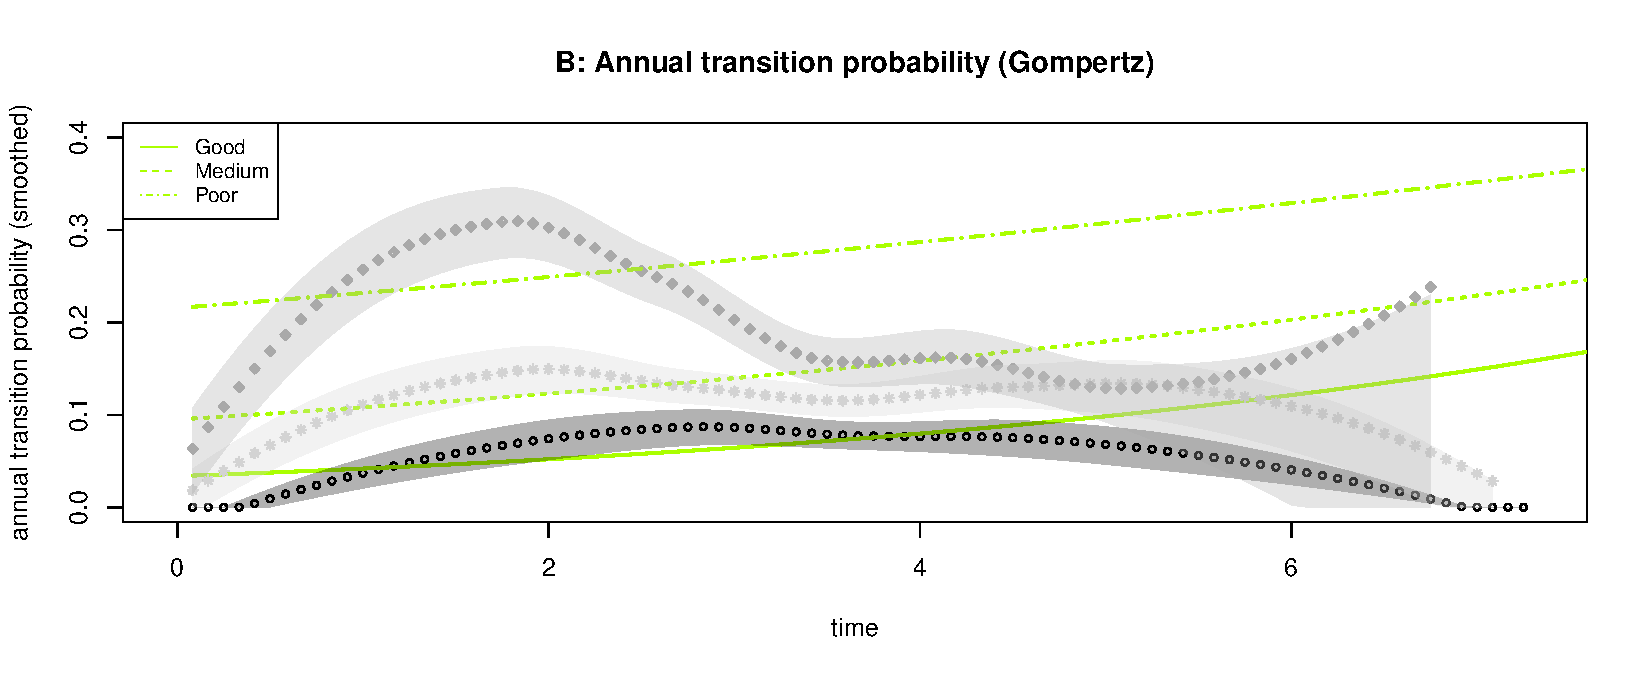
\includegraphics[height=0.3\textheight]{Images/gom-2} \end{flushleft}

\begin{flushleft}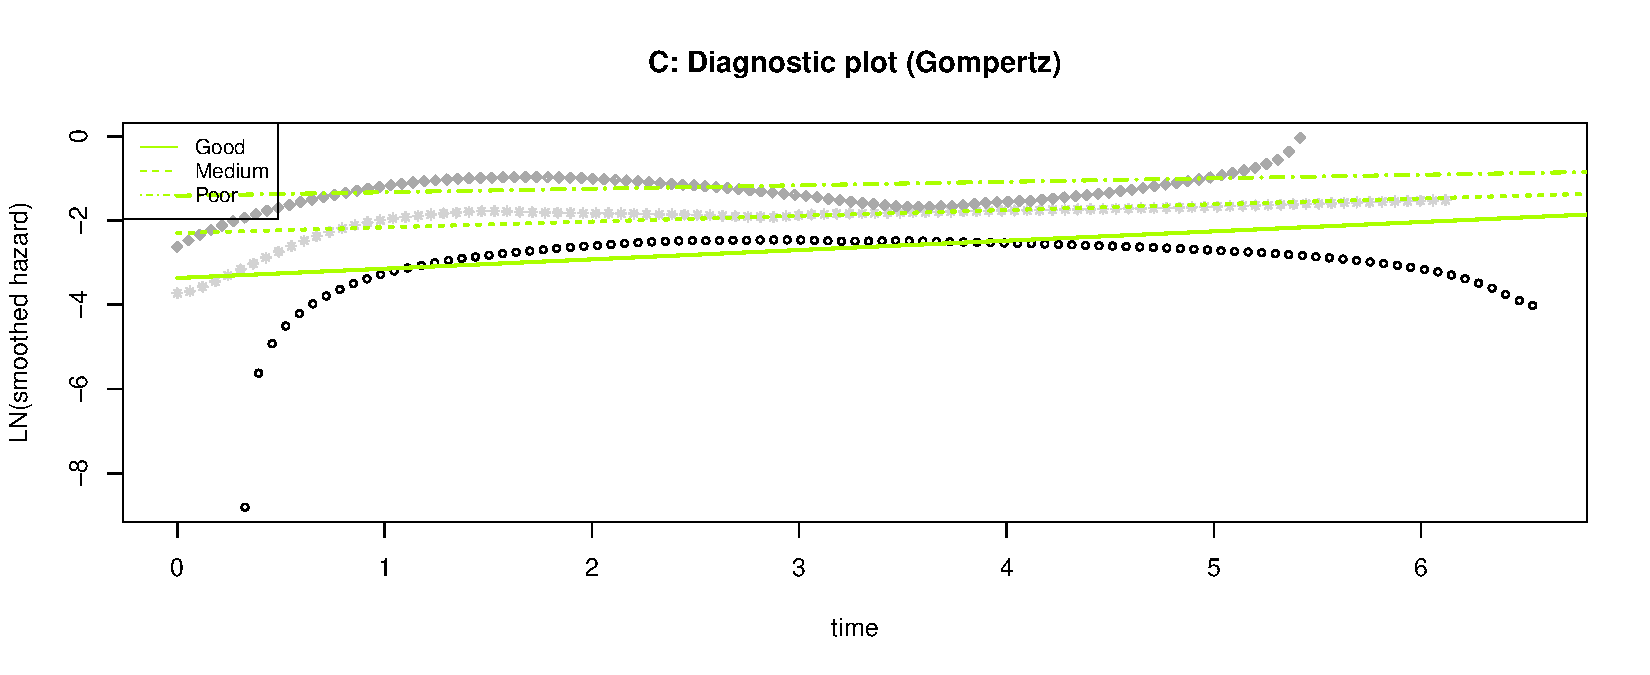
\includegraphics[height=0.3\textheight]{Images/gom-3} \end{flushleft}

\subsection{Log-normal}\label{log-normal}

\begin{flushleft}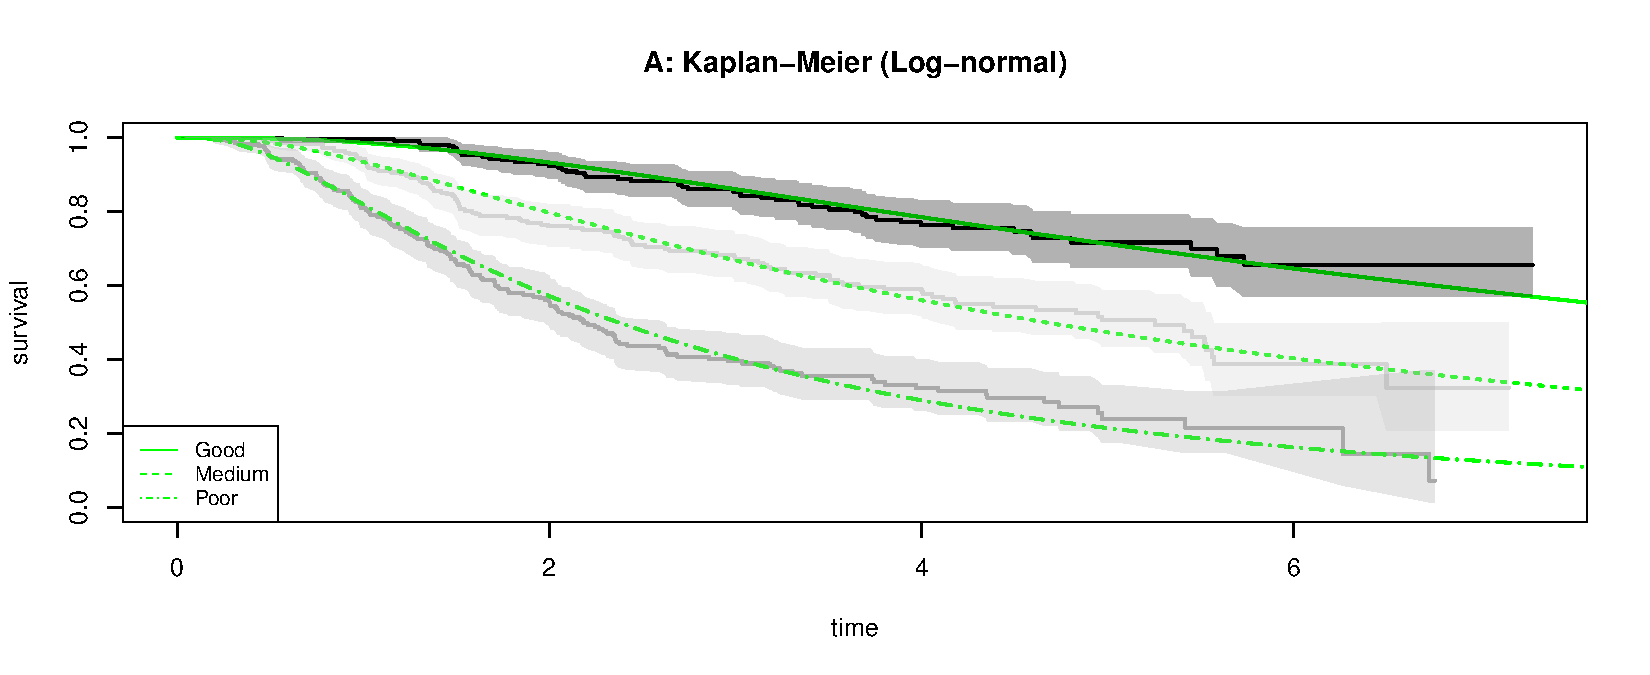
\includegraphics[height=0.3\textheight]{Images/lnorm-1} \end{flushleft}

\begin{flushleft}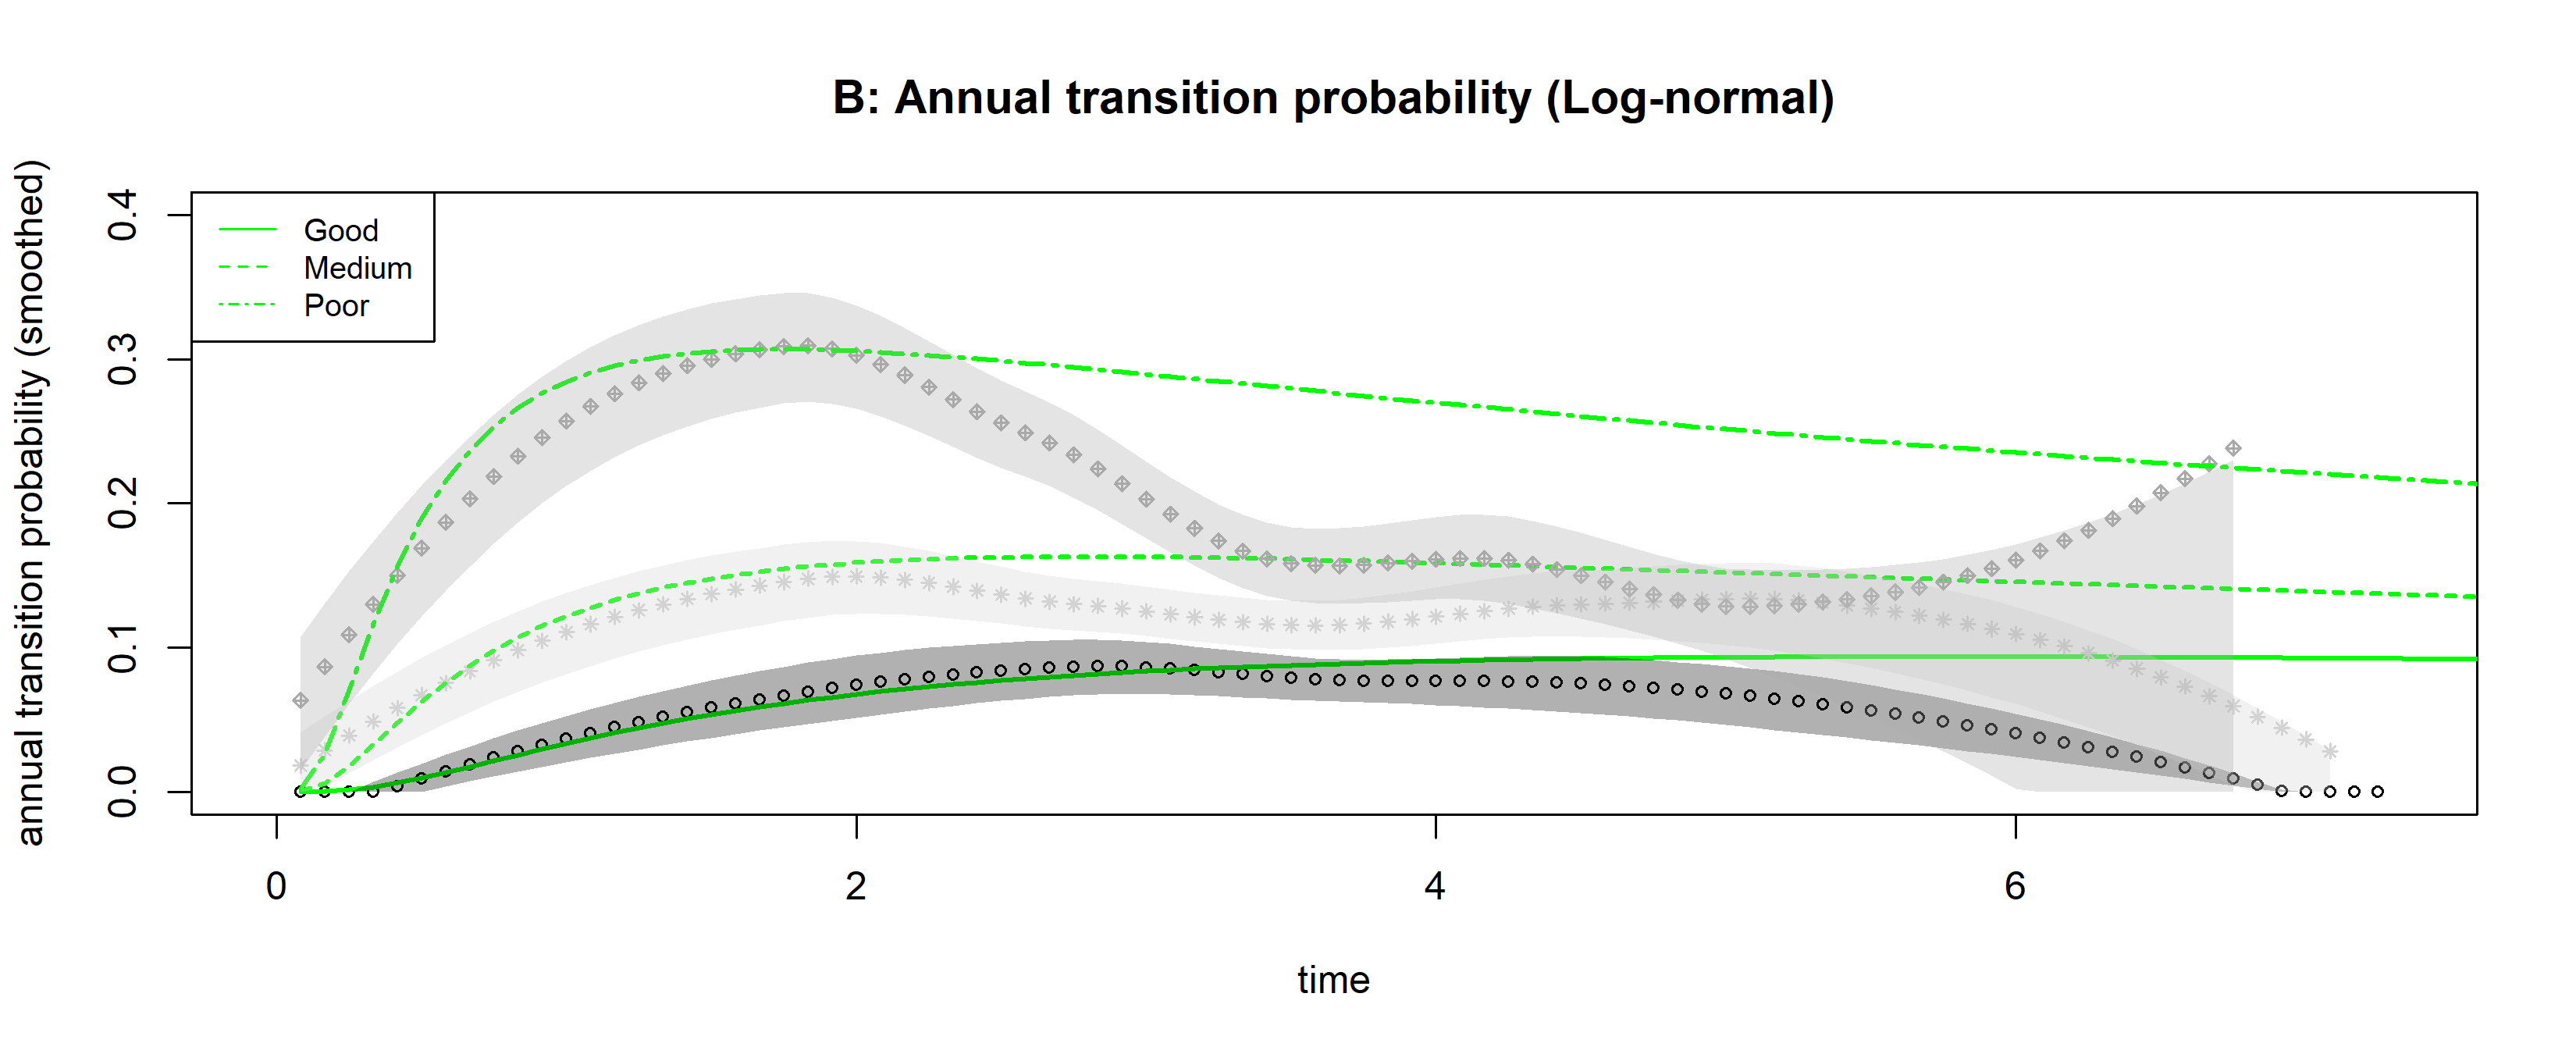
\includegraphics[height=0.3\textheight]{Images/lnorm-2} \end{flushleft}

\begin{flushleft}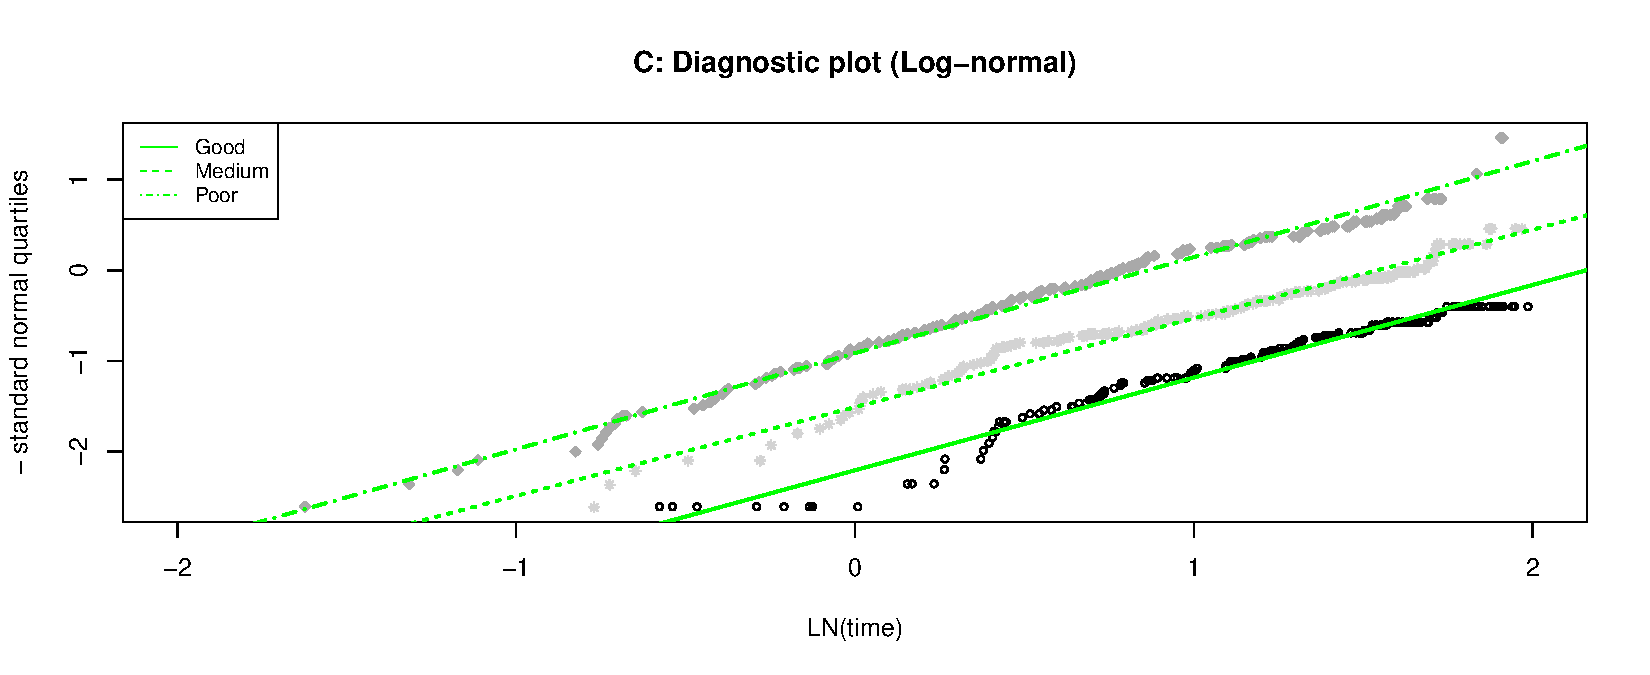
\includegraphics[height=0.3\textheight]{Images/lnorm-3} \end{flushleft}

\subsection{Log-logistic}\label{log-logistic}

\begin{flushleft}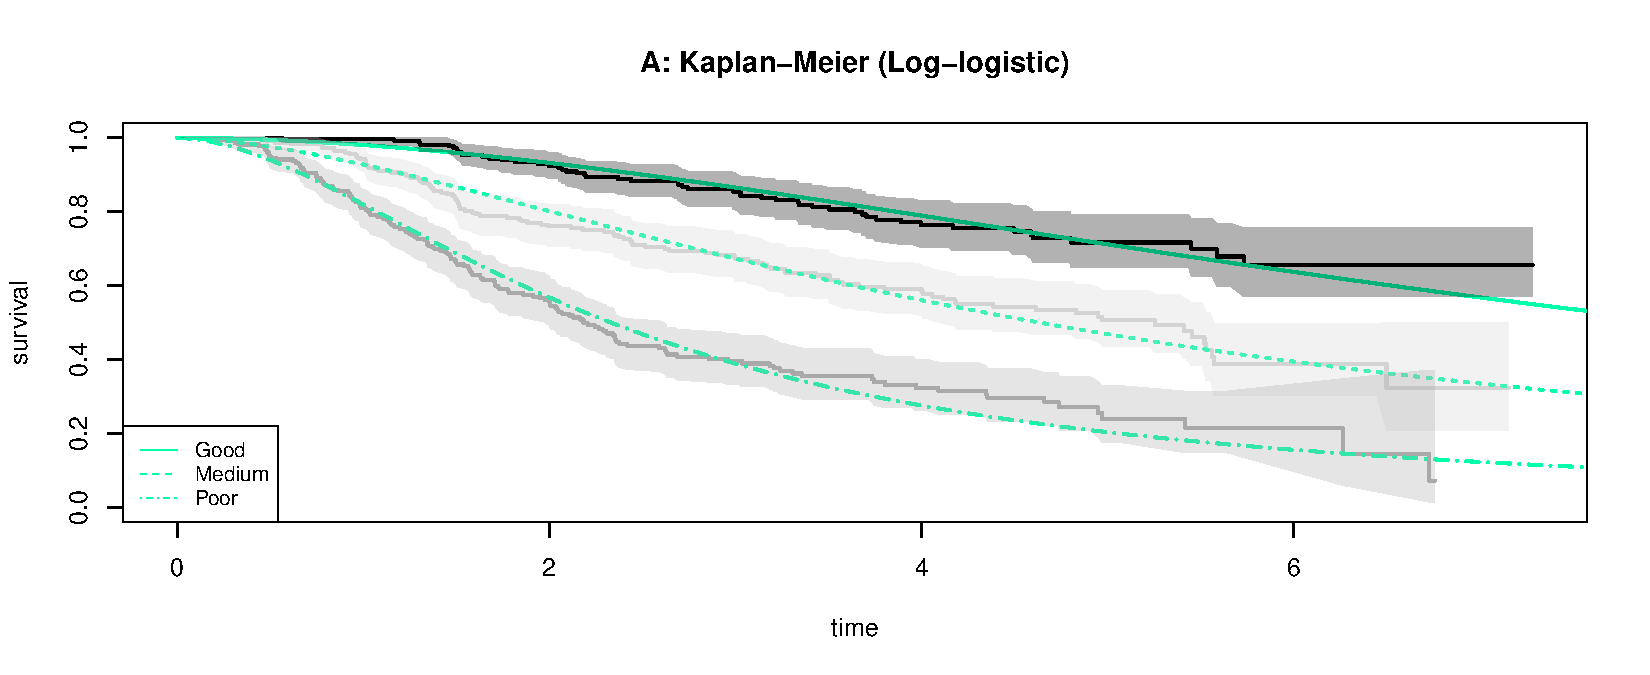
\includegraphics[height=0.3\textheight]{Images/llog-1} \end{flushleft}

\begin{flushleft}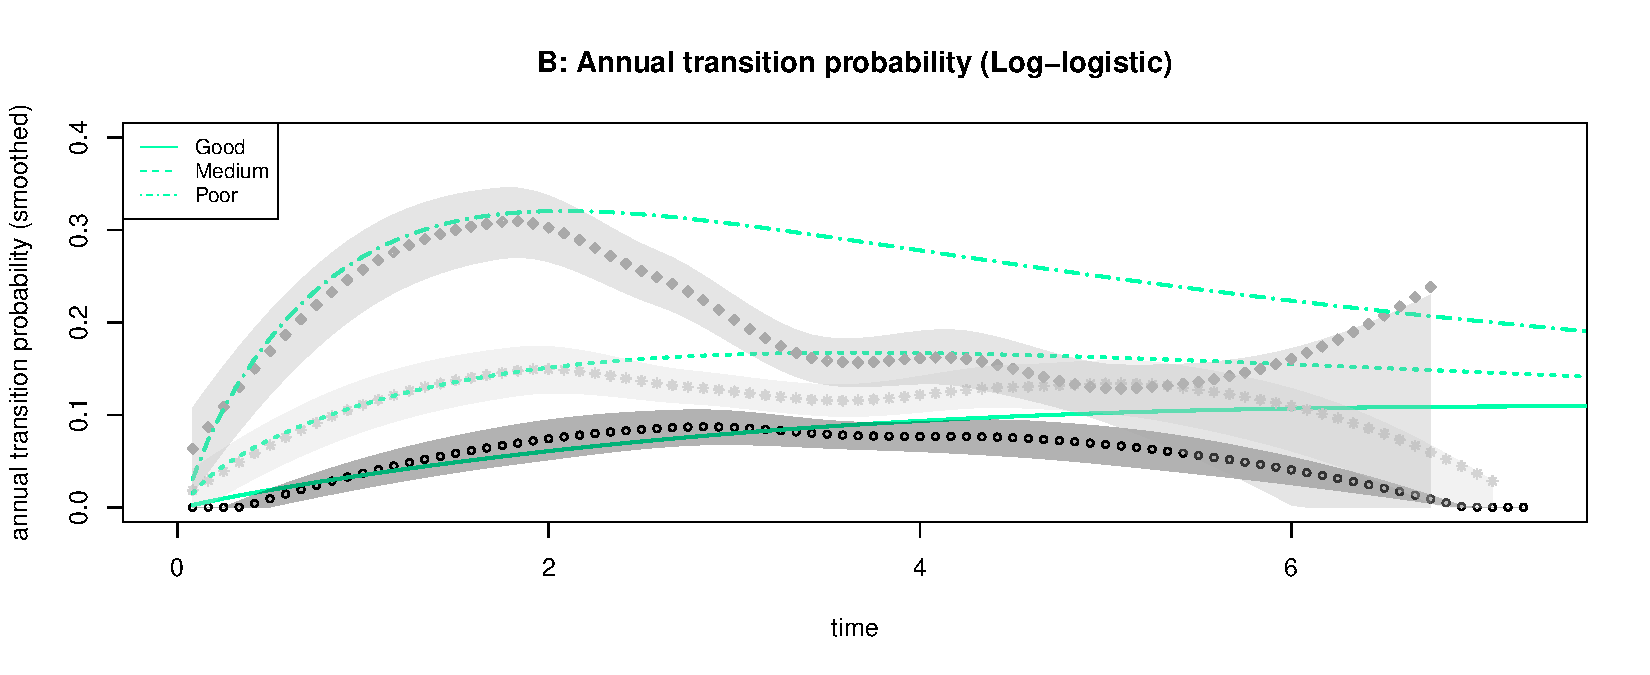
\includegraphics[height=0.3\textheight]{Images/llog-2} \end{flushleft}

\begin{flushleft}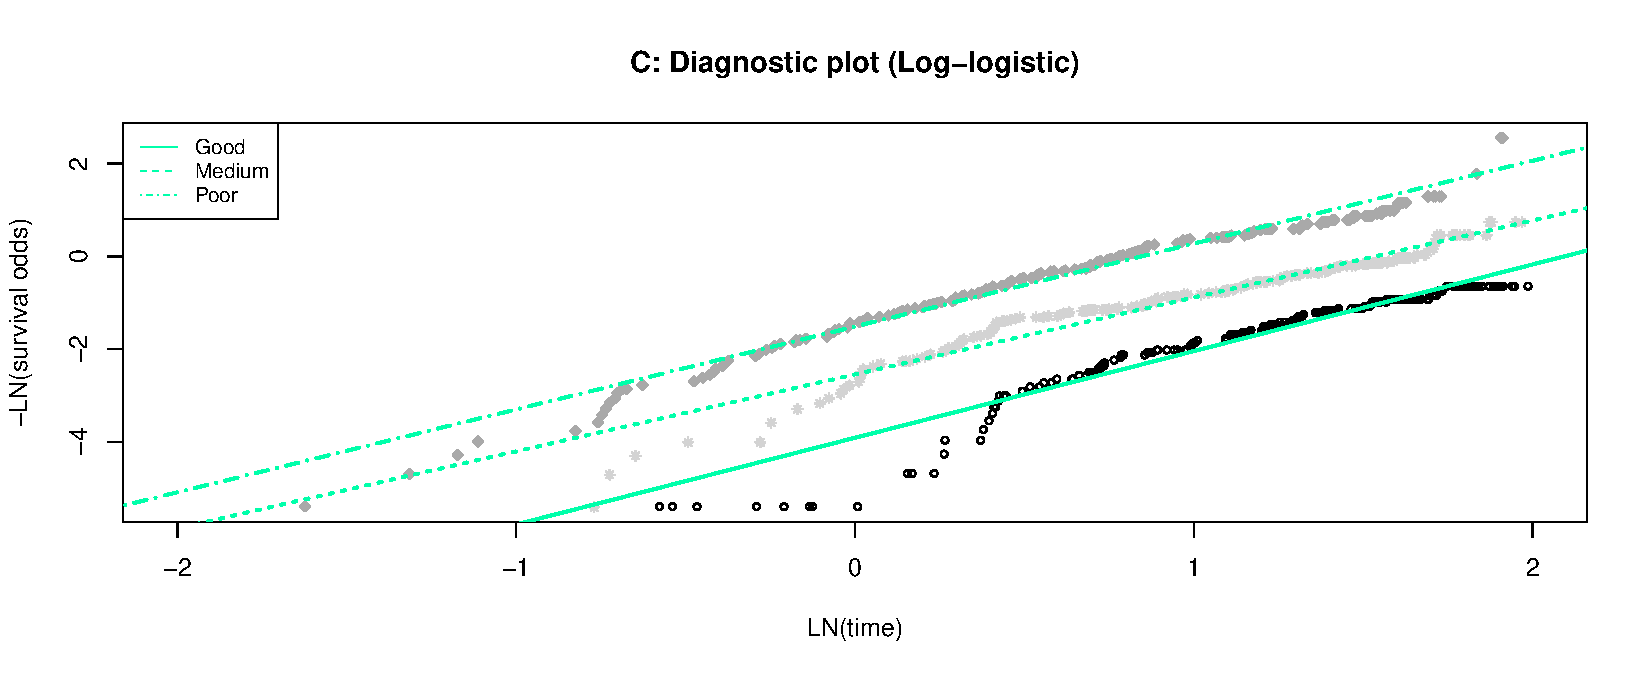
\includegraphics[height=0.3\textheight]{Images/llog-3} \end{flushleft}

\subsection{Gamma}\label{gamma}

\begin{flushleft}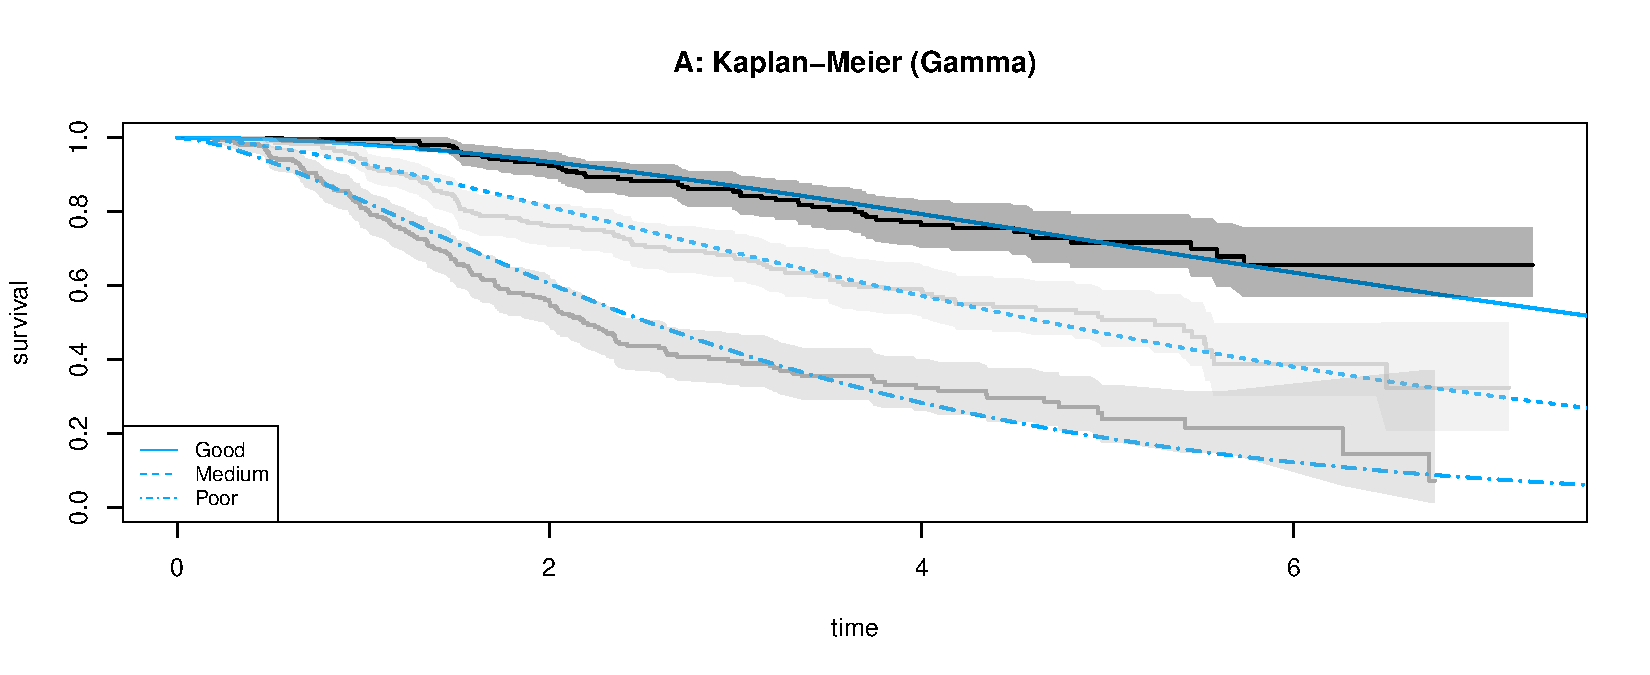
\includegraphics[height=0.3\textheight]{Images/gam-1} \end{flushleft}

\begin{flushleft}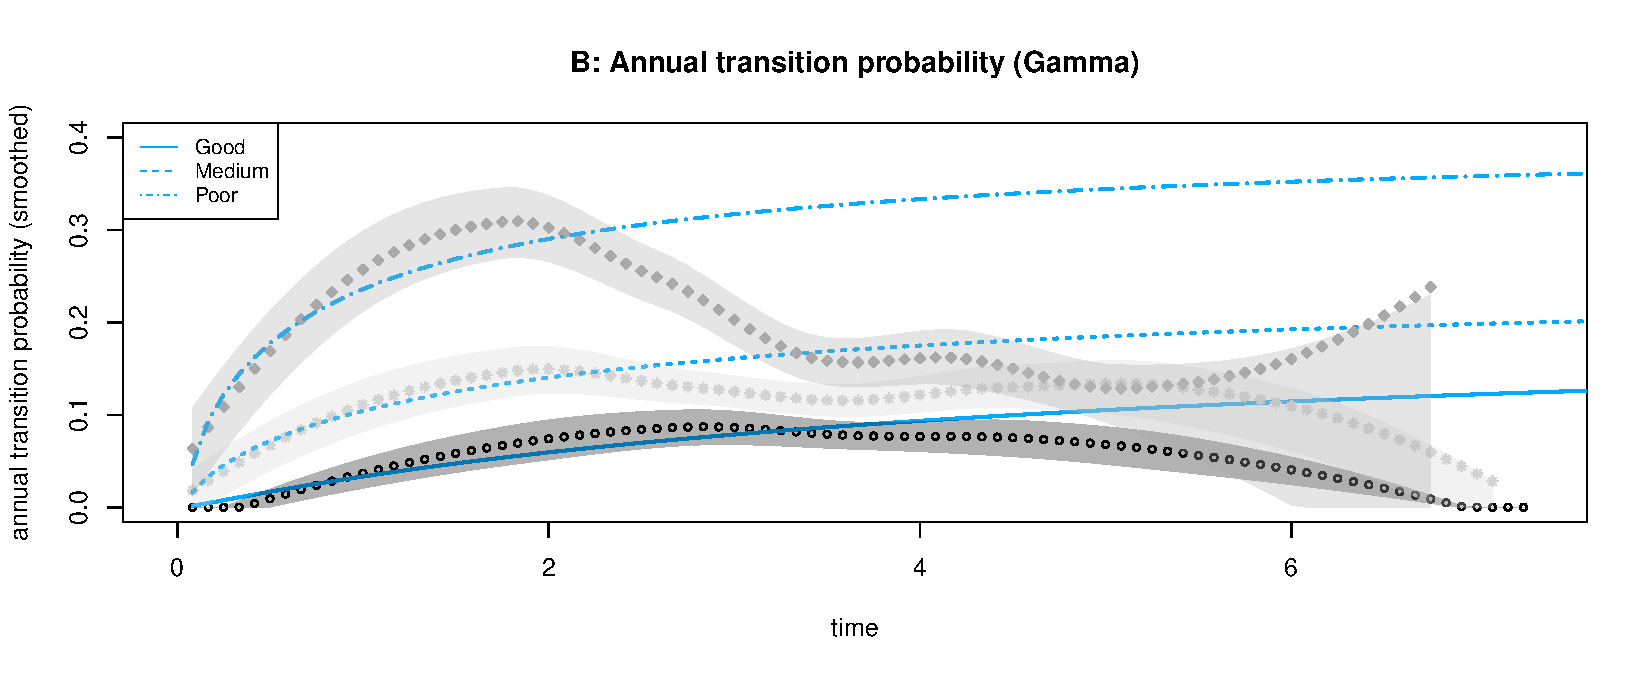
\includegraphics[height=0.3\textheight]{Images/gam-2} \end{flushleft}

\begin{flushleft}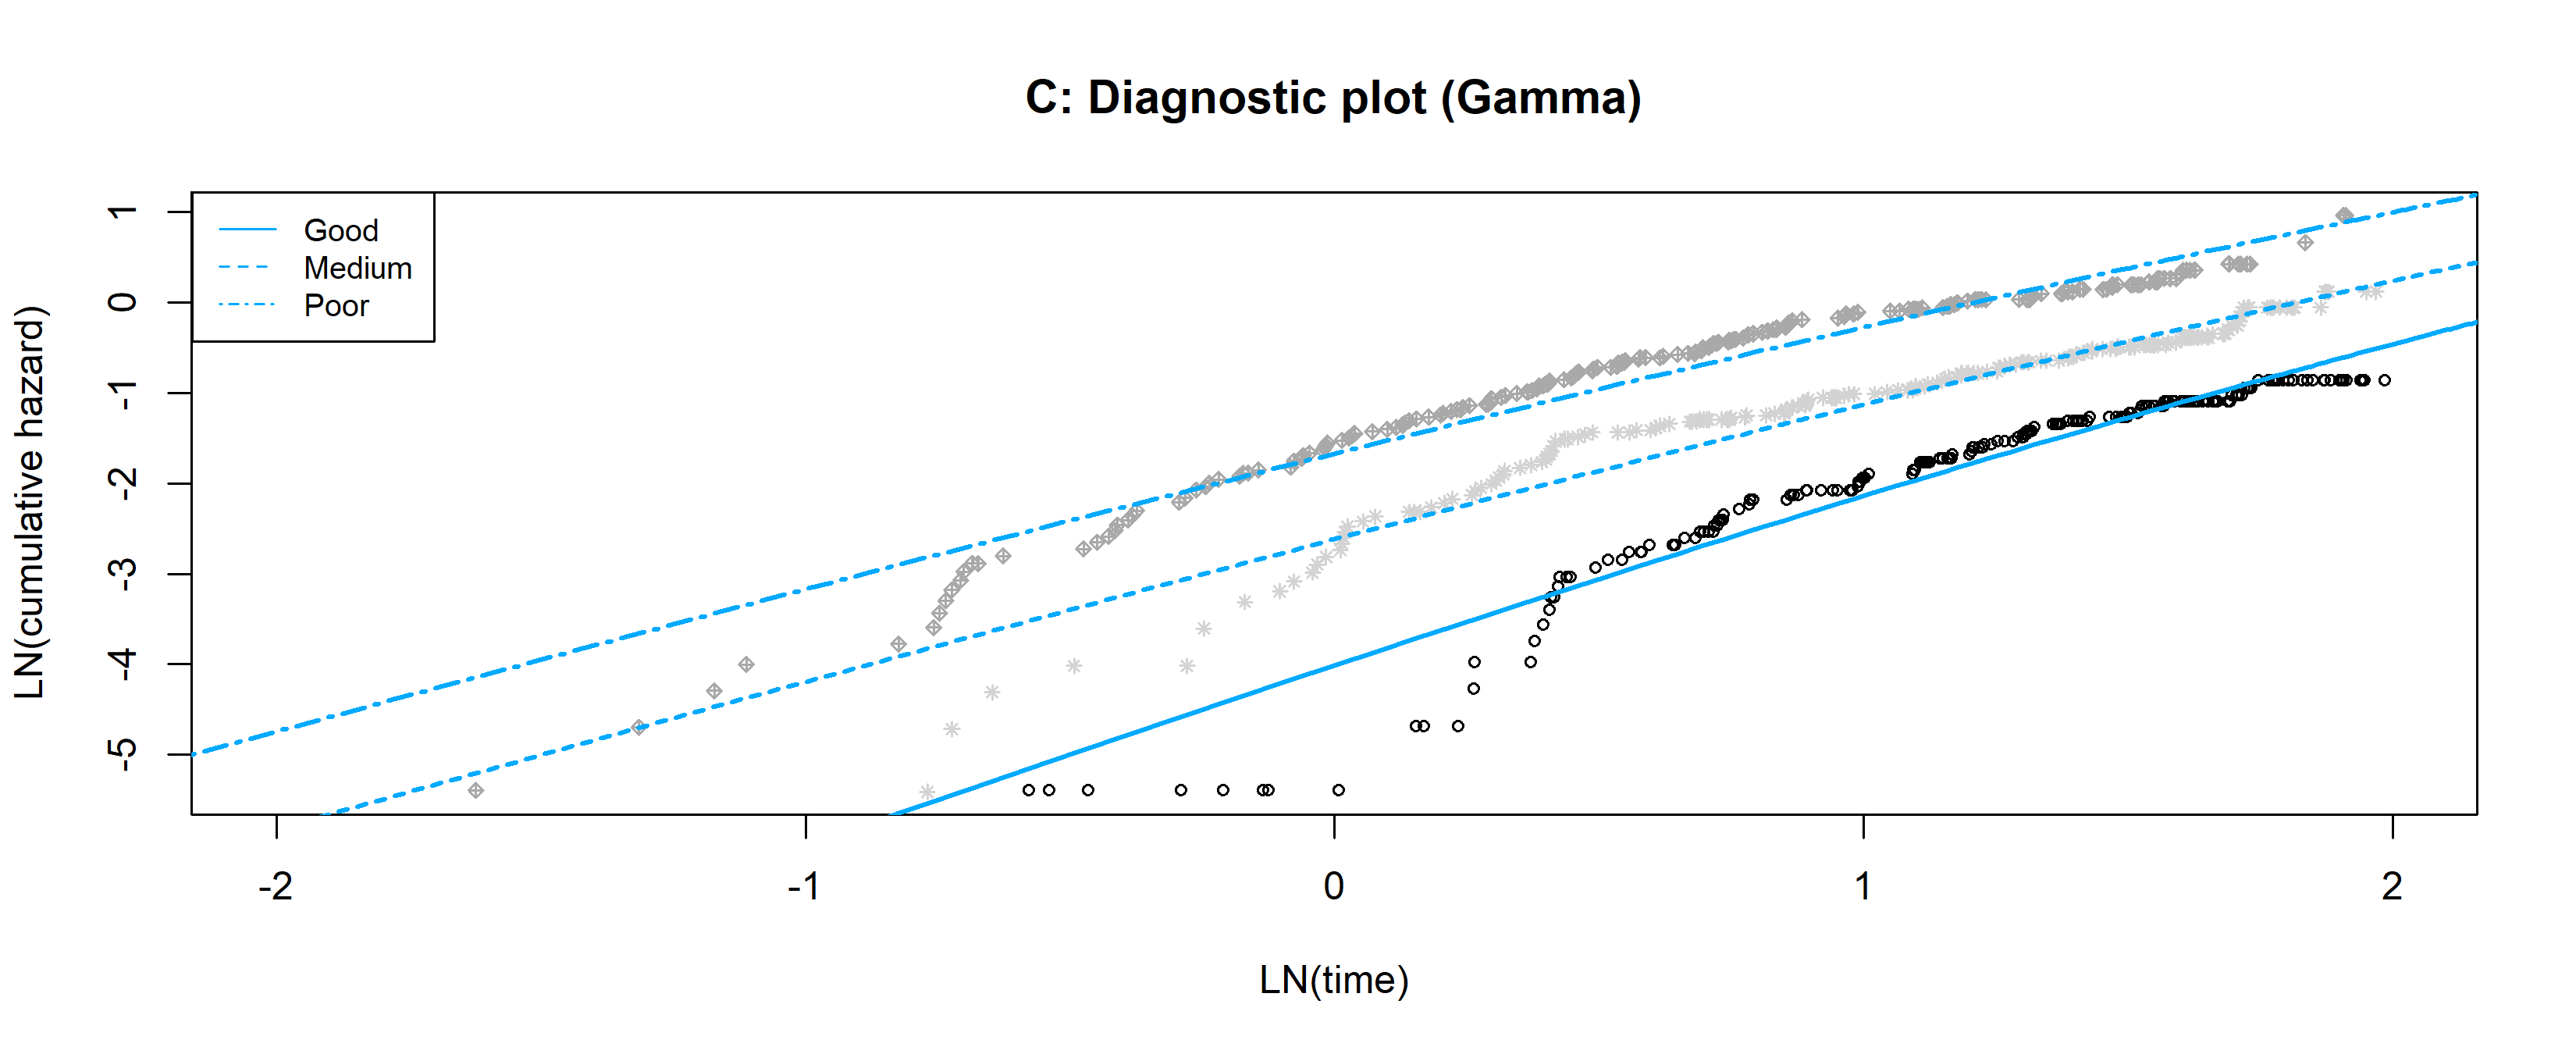
\includegraphics[height=0.3\textheight]{Images/gam-3} \end{flushleft}

\subsection{Generalised Gamma}\label{generalised-gamma}

\begin{flushleft}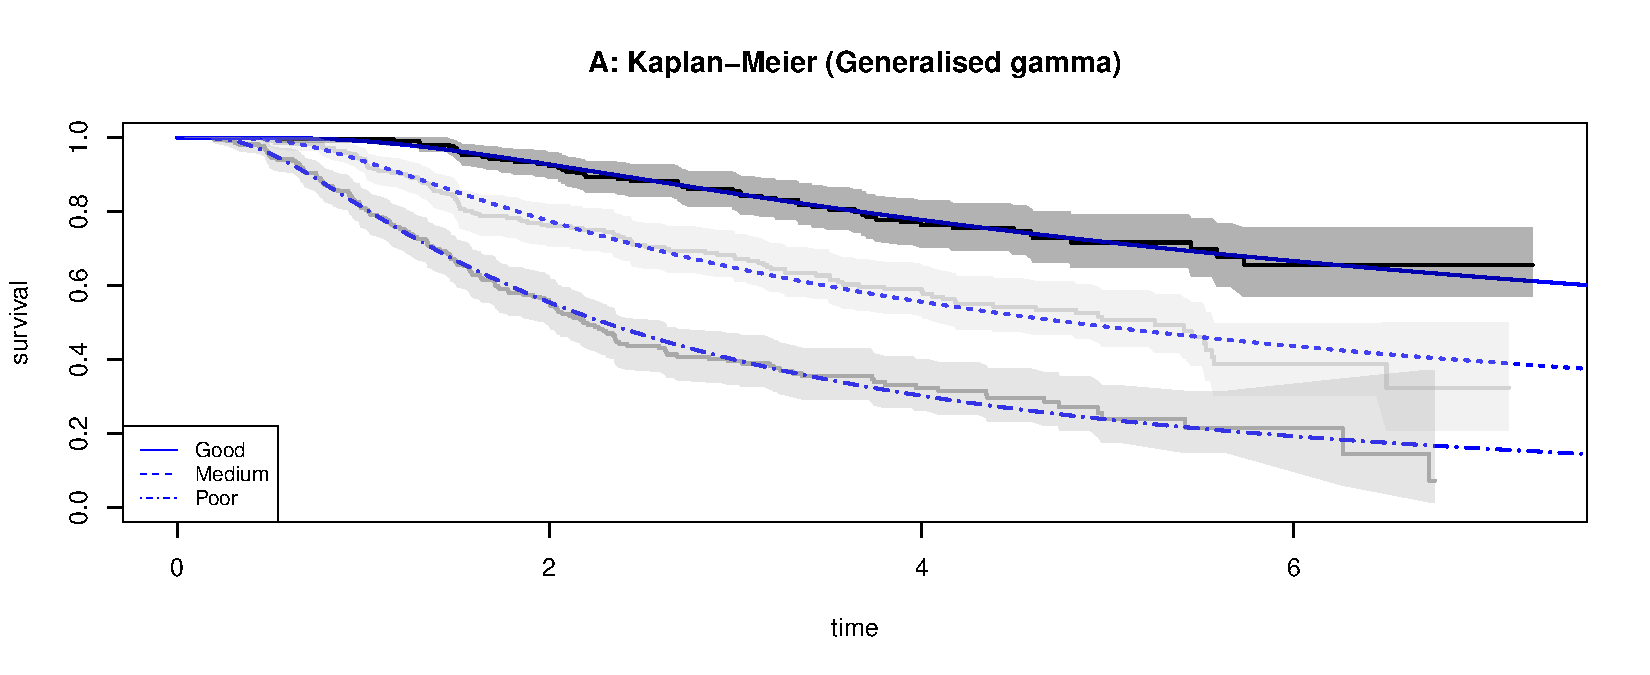
\includegraphics[height=0.3\textheight]{Images/ggam-1} \end{flushleft}

\begin{flushleft}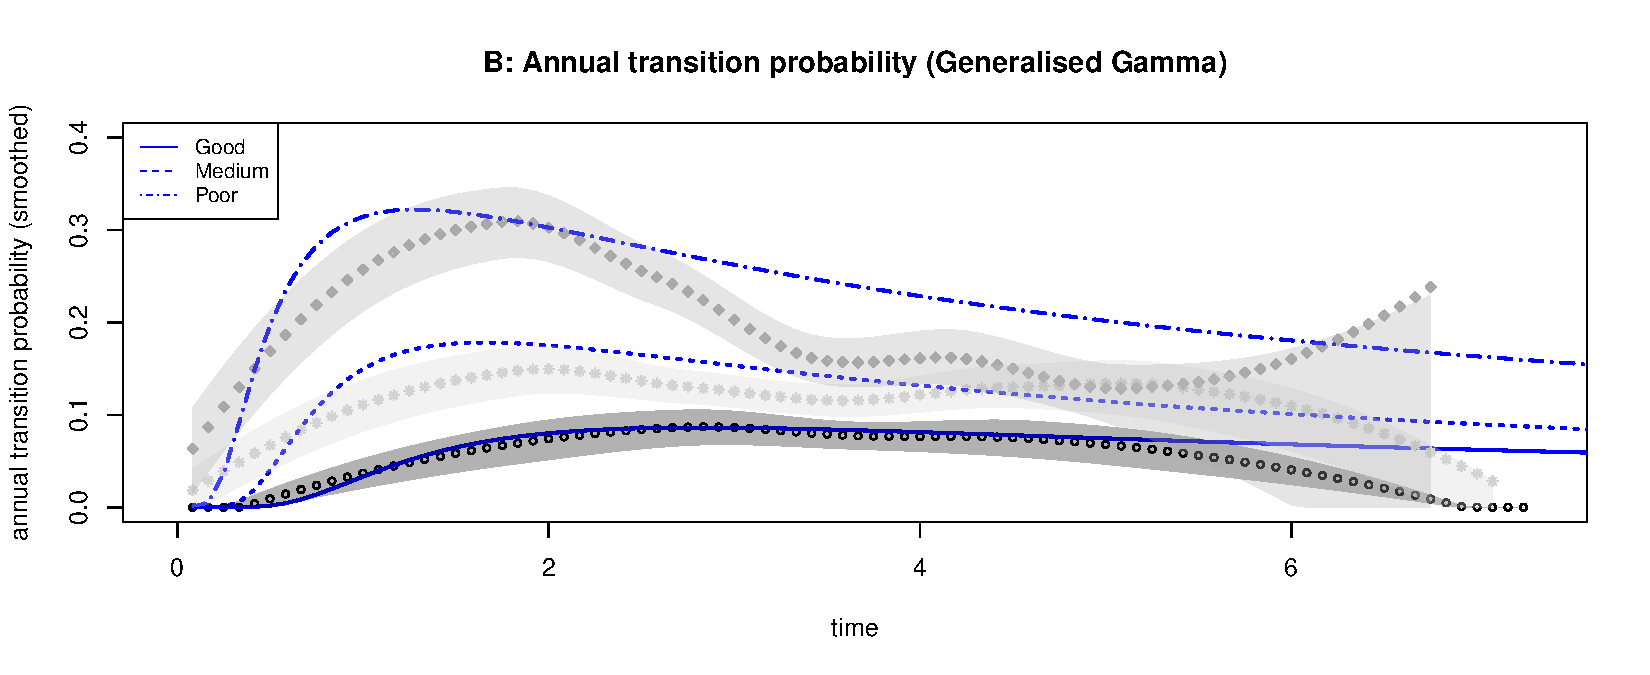
\includegraphics[height=0.3\textheight]{Images/ggam-2} \end{flushleft}

\begin{flushleft}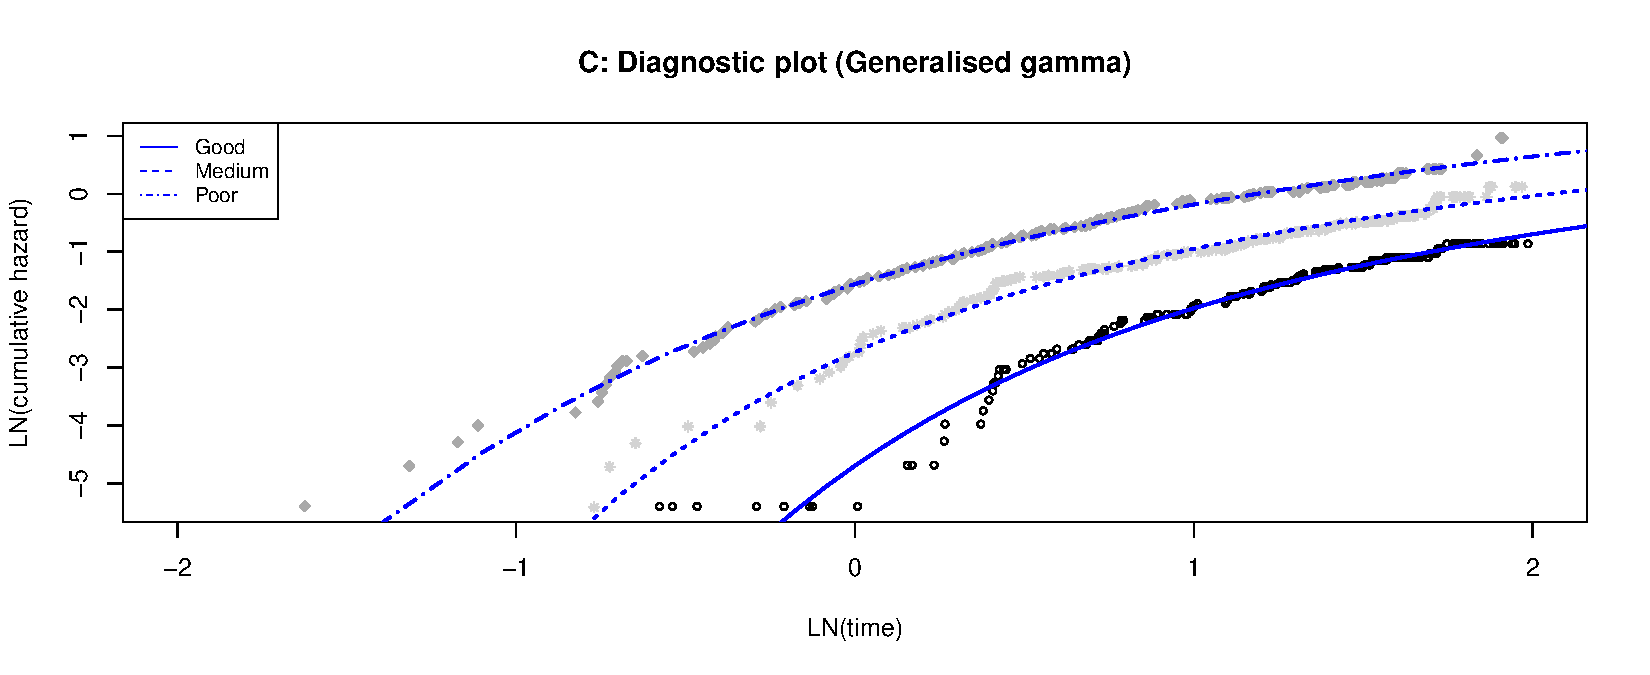
\includegraphics[height=0.3\textheight]{Images/ggam-3} \end{flushleft}

\newpage

\section{Parametric spline models?}\label{parametric-spline-models}

If standard parametric models are not appropriate, are spline models a
more appropriate fit to the data?

\begin{flushleft}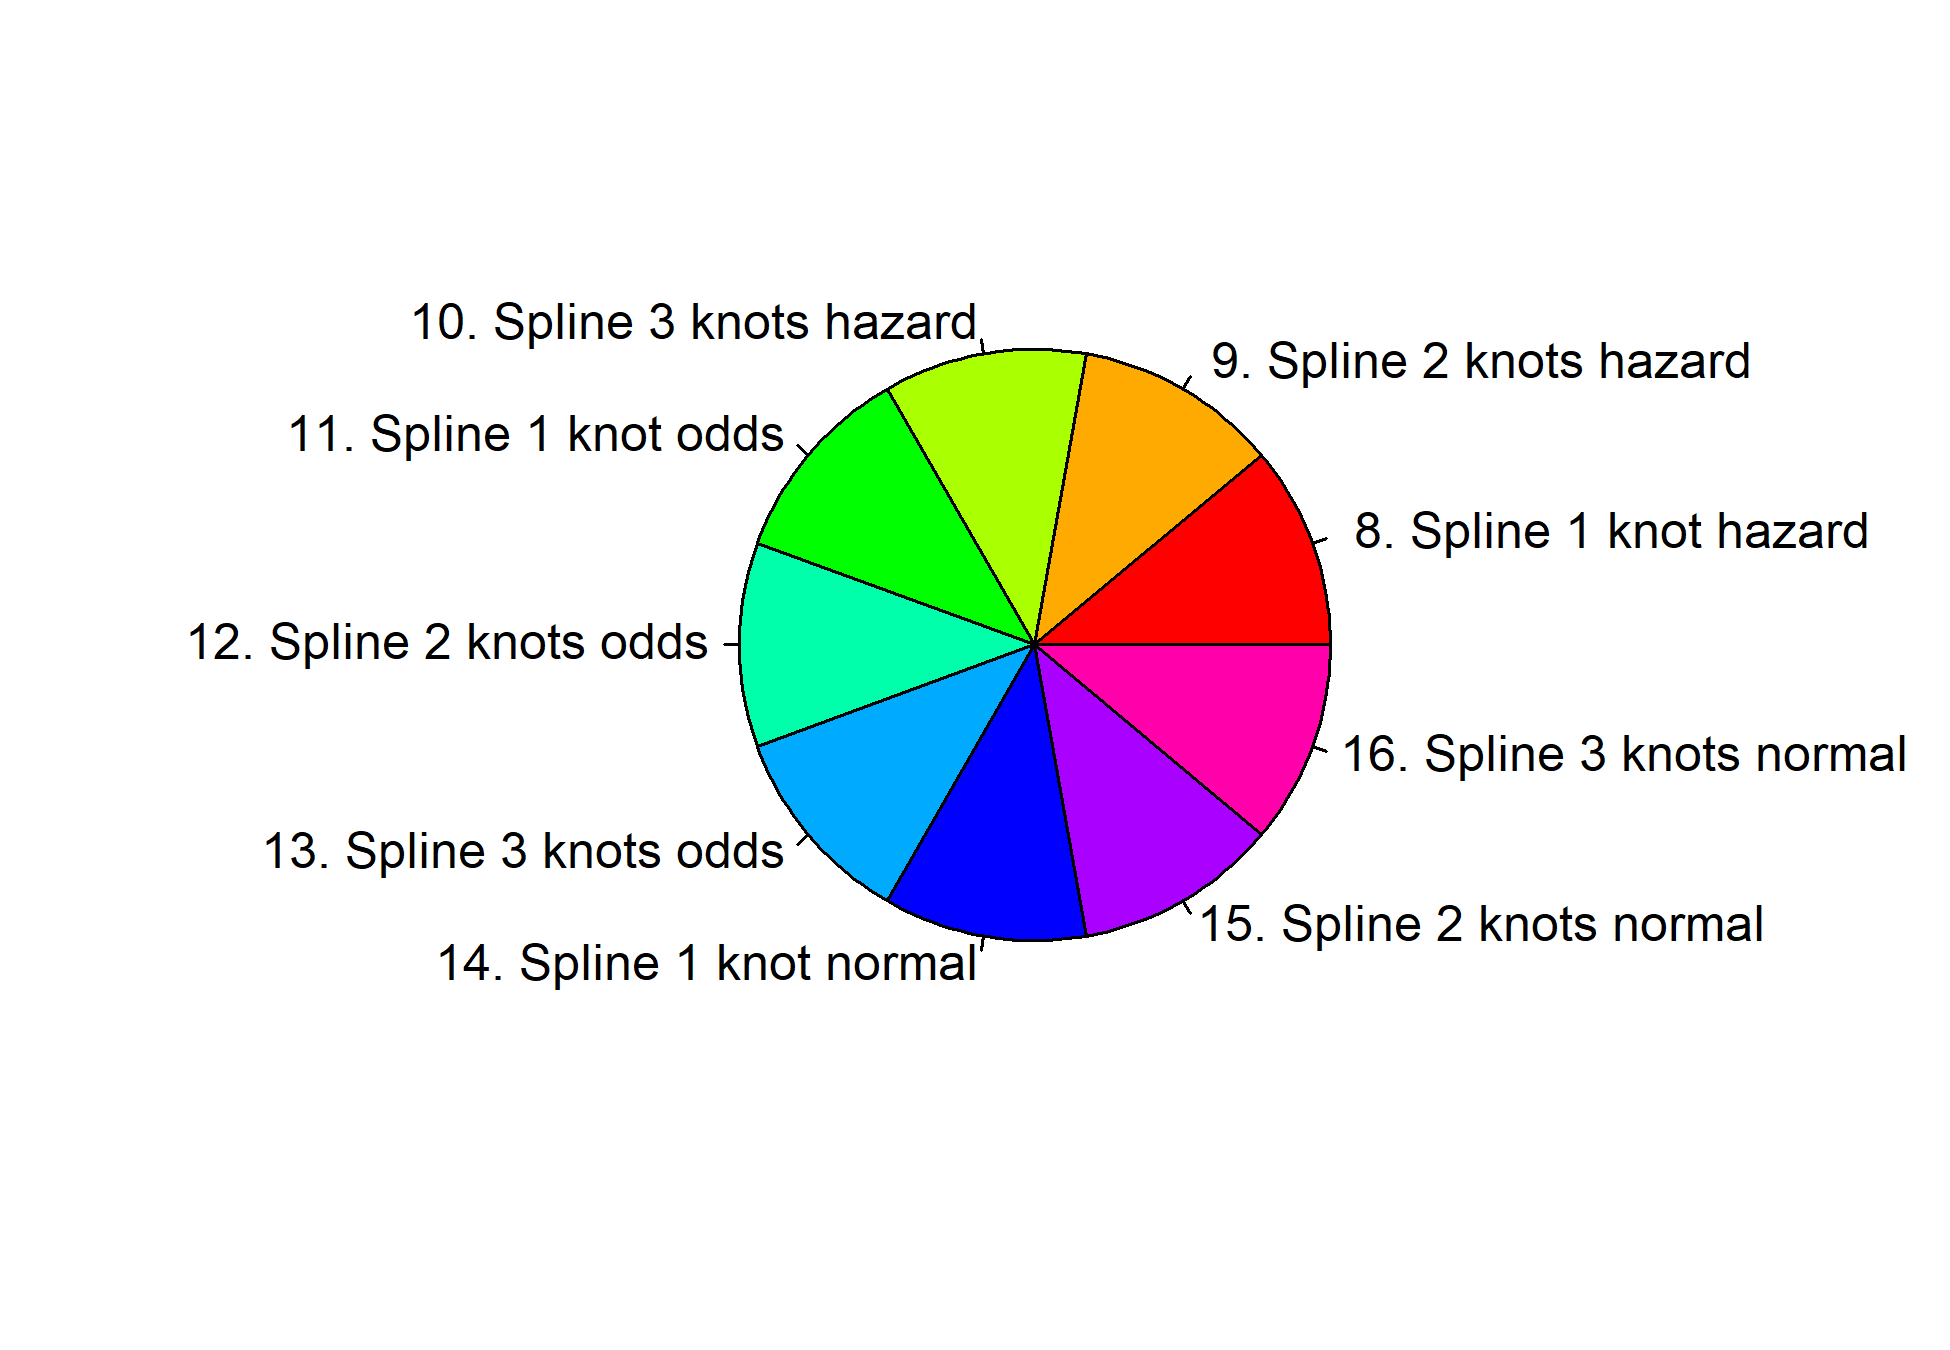
\includegraphics{Images/spline-1} \end{flushleft}

\begin{table}[H]
\centering
\begin{tabular}{lrr}
\toprule
Model & AIC & BIC\\
\midrule
\cellcolor{gray!6}{9. Spline 2 knots hazard} & \cellcolor{gray!6}{1585.894} & \cellcolor{gray!6}{1640.264}\\
11. Spline 2 knots odds & 1587.289 & 1641.659\\
\cellcolor{gray!6}{12. Spline 1 knot normal} & \cellcolor{gray!6}{1587.682} & \cellcolor{gray!6}{1628.460}\\
13. Spline 2 knots normal & 1588.343 & 1642.714\\
\cellcolor{gray!6}{7. Generalised Gamma} & \cellcolor{gray!6}{1589.049} & \cellcolor{gray!6}{1629.826}\\
8. Spline 1 knot hazard & 1589.327 & 1630.105\\
\cellcolor{gray!6}{10. Spline 1 knot odds} & \cellcolor{gray!6}{1590.221} & \cellcolor{gray!6}{1630.999}\\
4. Log-normal & 1592.880 & 1620.066\\
\cellcolor{gray!6}{5. Log-logistic} & \cellcolor{gray!6}{1609.294} & \cellcolor{gray!6}{1636.479}\\
6. Gamma & 1621.982 & 1649.167\\
\cellcolor{gray!6}{2. Weibull} & \cellcolor{gray!6}{1632.618} & \cellcolor{gray!6}{1659.803}\\
3. Gompertz & 1660.954 & 1688.140\\
\cellcolor{gray!6}{1. Exponential} & \cellcolor{gray!6}{1668.212} & \cellcolor{gray!6}{1681.805}\\
\bottomrule
\end{tabular}
\end{table}

\subsection{Spline hazard 1 knot}\label{spline-hazard-1-knot}

\begin{flushleft}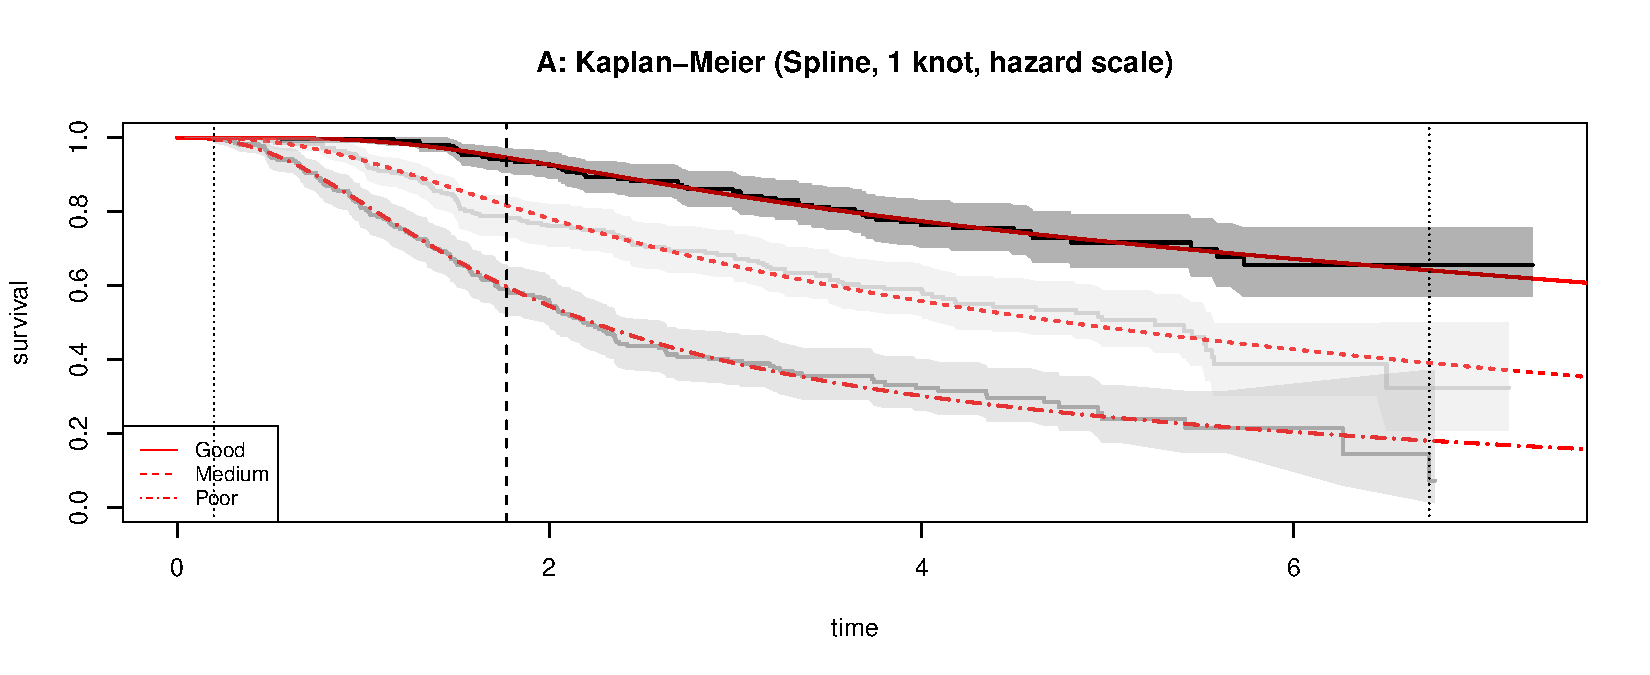
\includegraphics[height=0.3\textheight]{Images/spline_hazard1-1} \end{flushleft}

\begin{flushleft}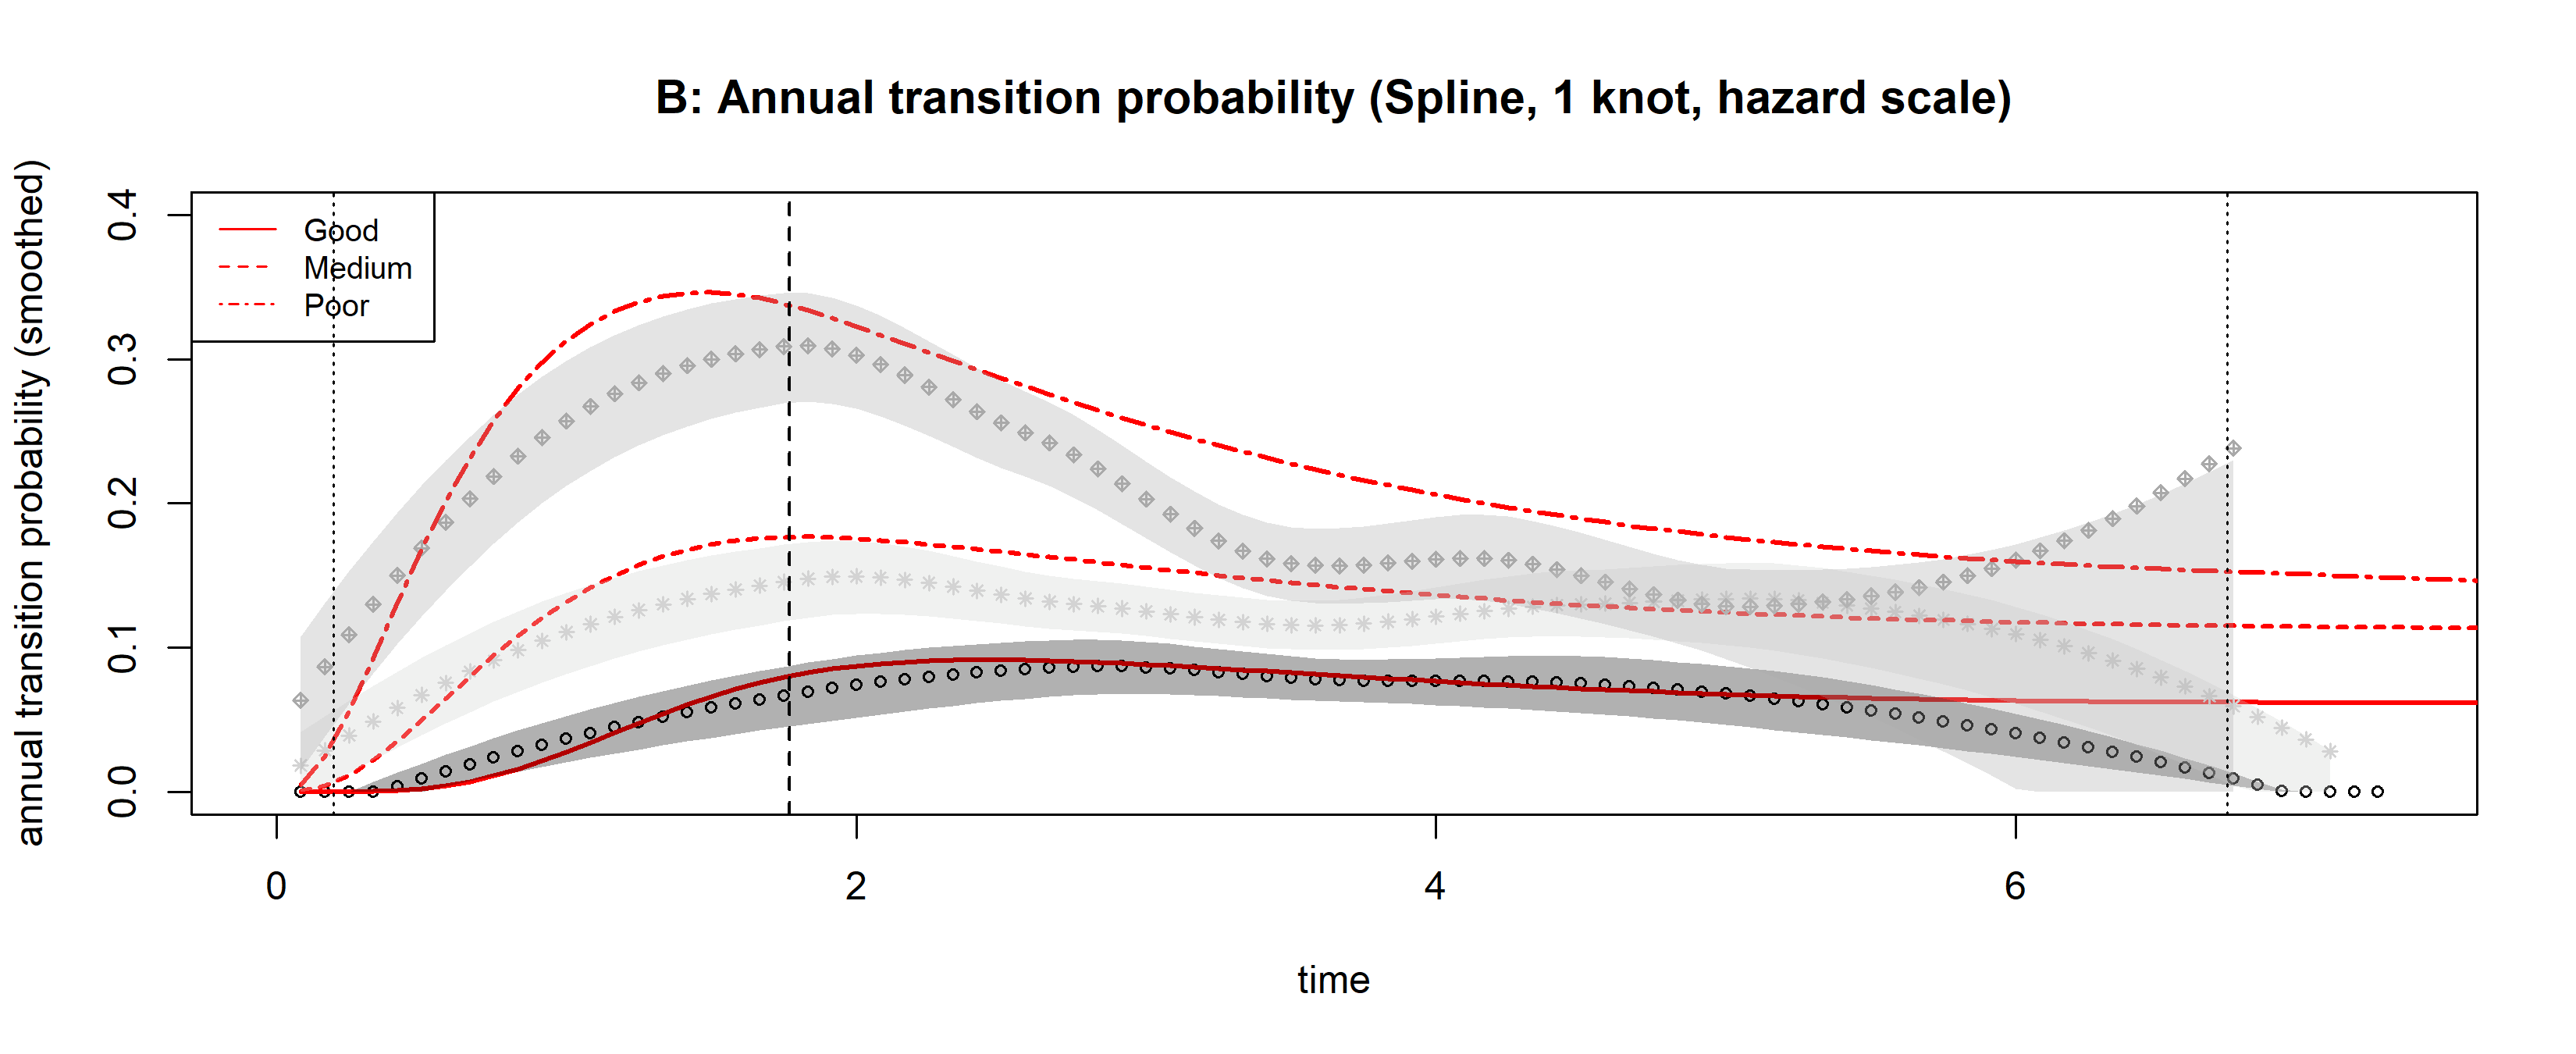
\includegraphics[height=0.3\textheight]{Images/spline_hazard1-2} \end{flushleft}

\begin{flushleft}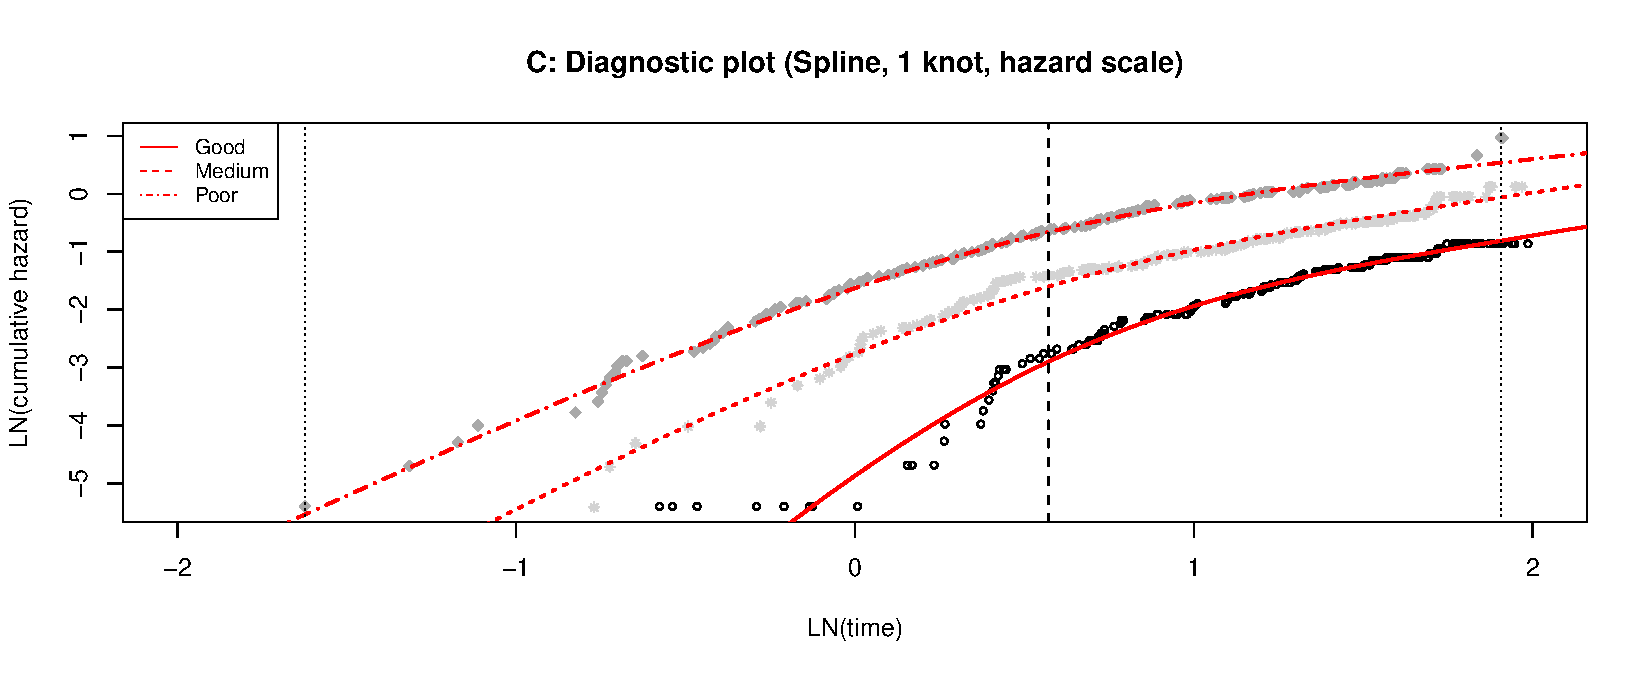
\includegraphics[height=0.3\textheight]{Images/spline_hazard1-3} \end{flushleft}

\subsection{Spline hazard 2 knots}\label{spline-hazard-2-knots}

\begin{flushleft}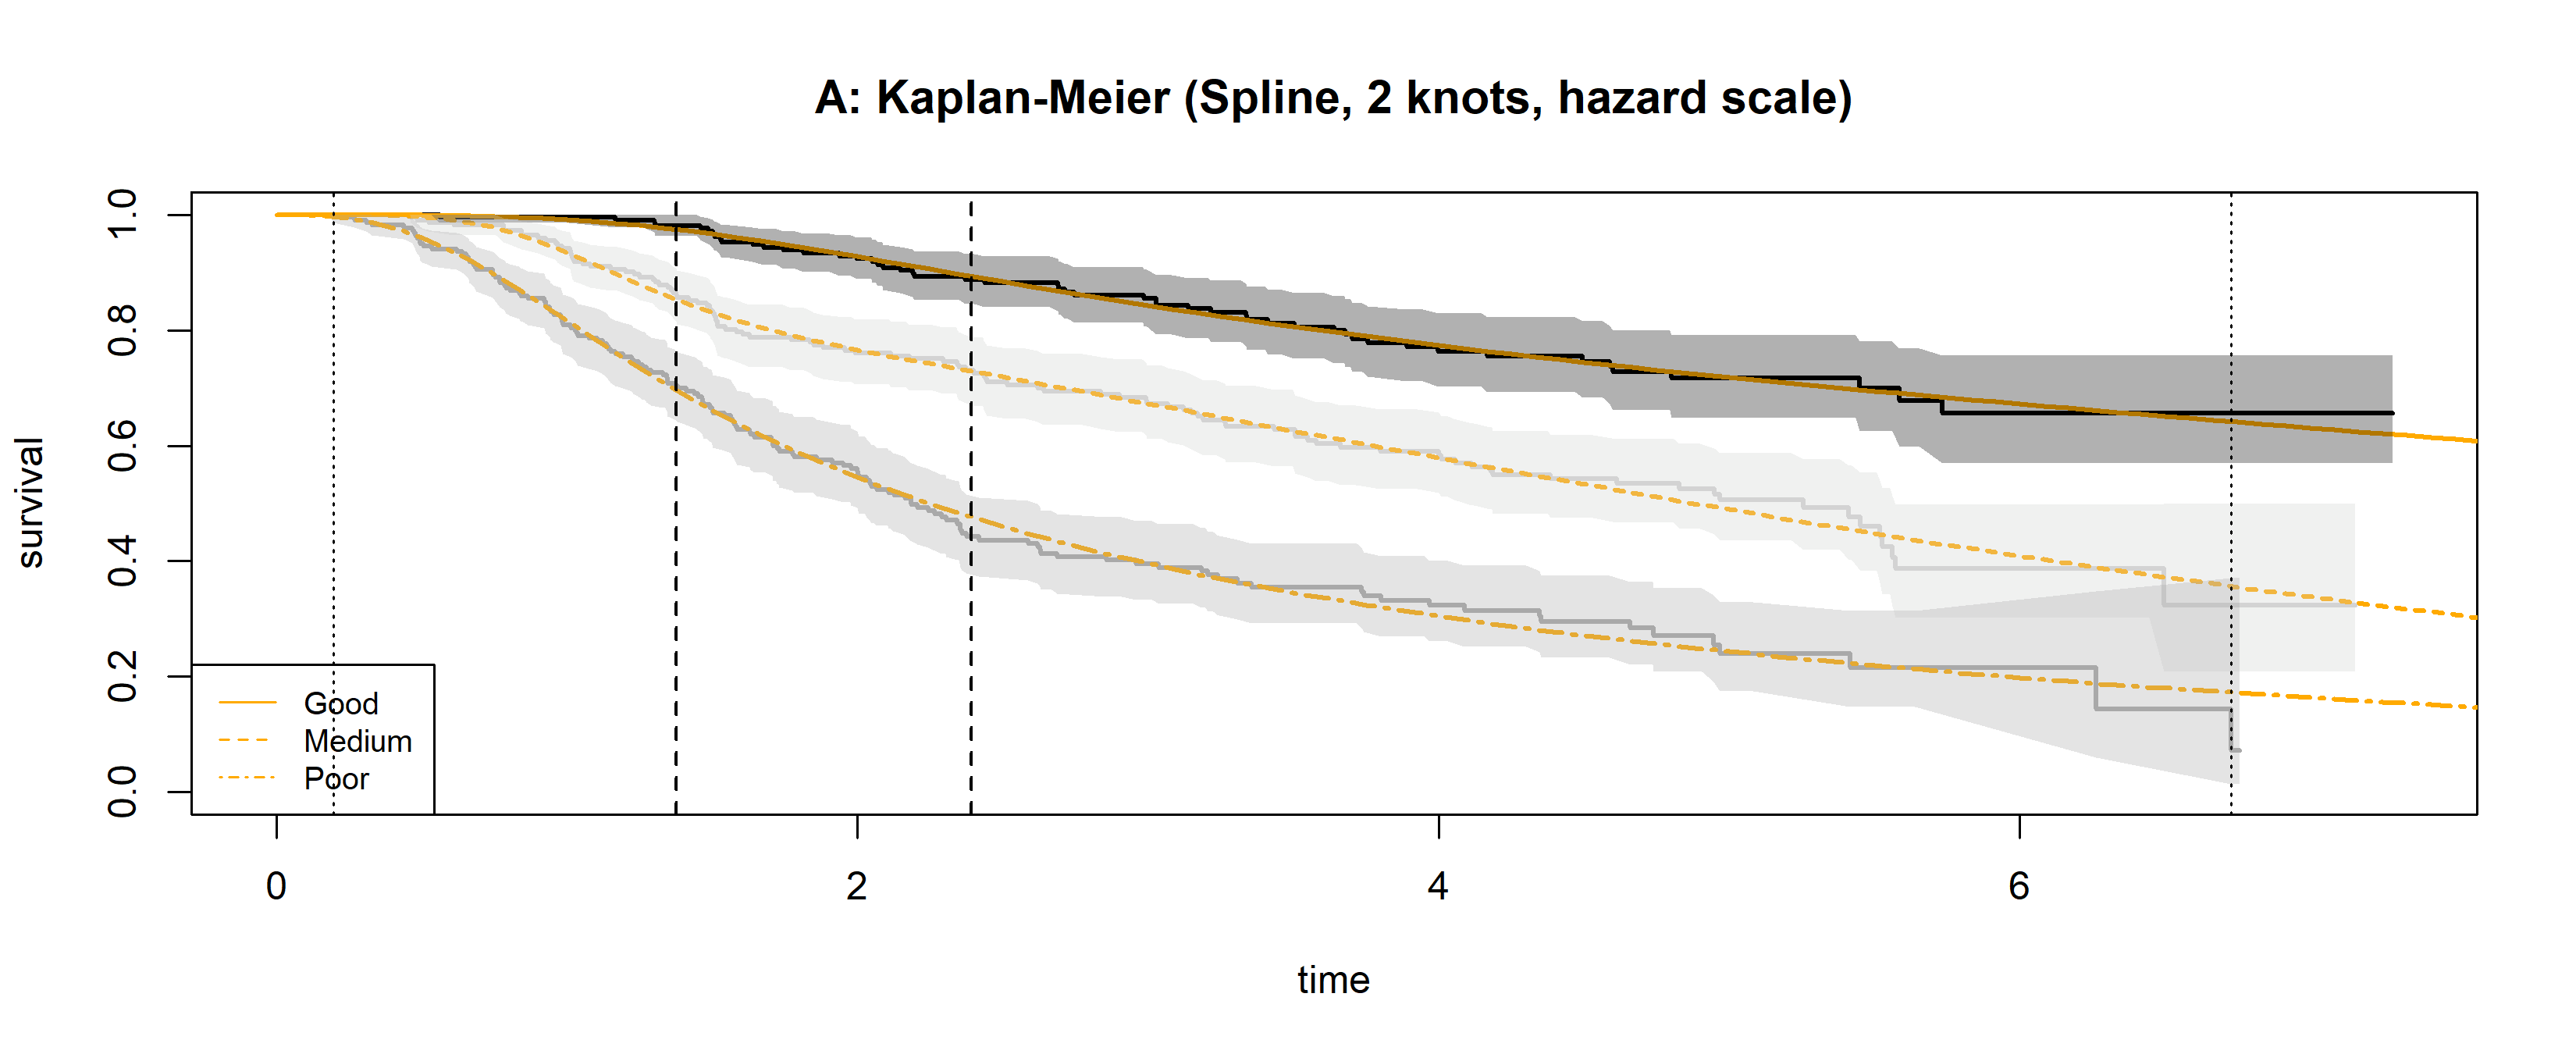
\includegraphics[height=0.3\textheight]{Images/spline_hazard2-1} \end{flushleft}

\begin{flushleft}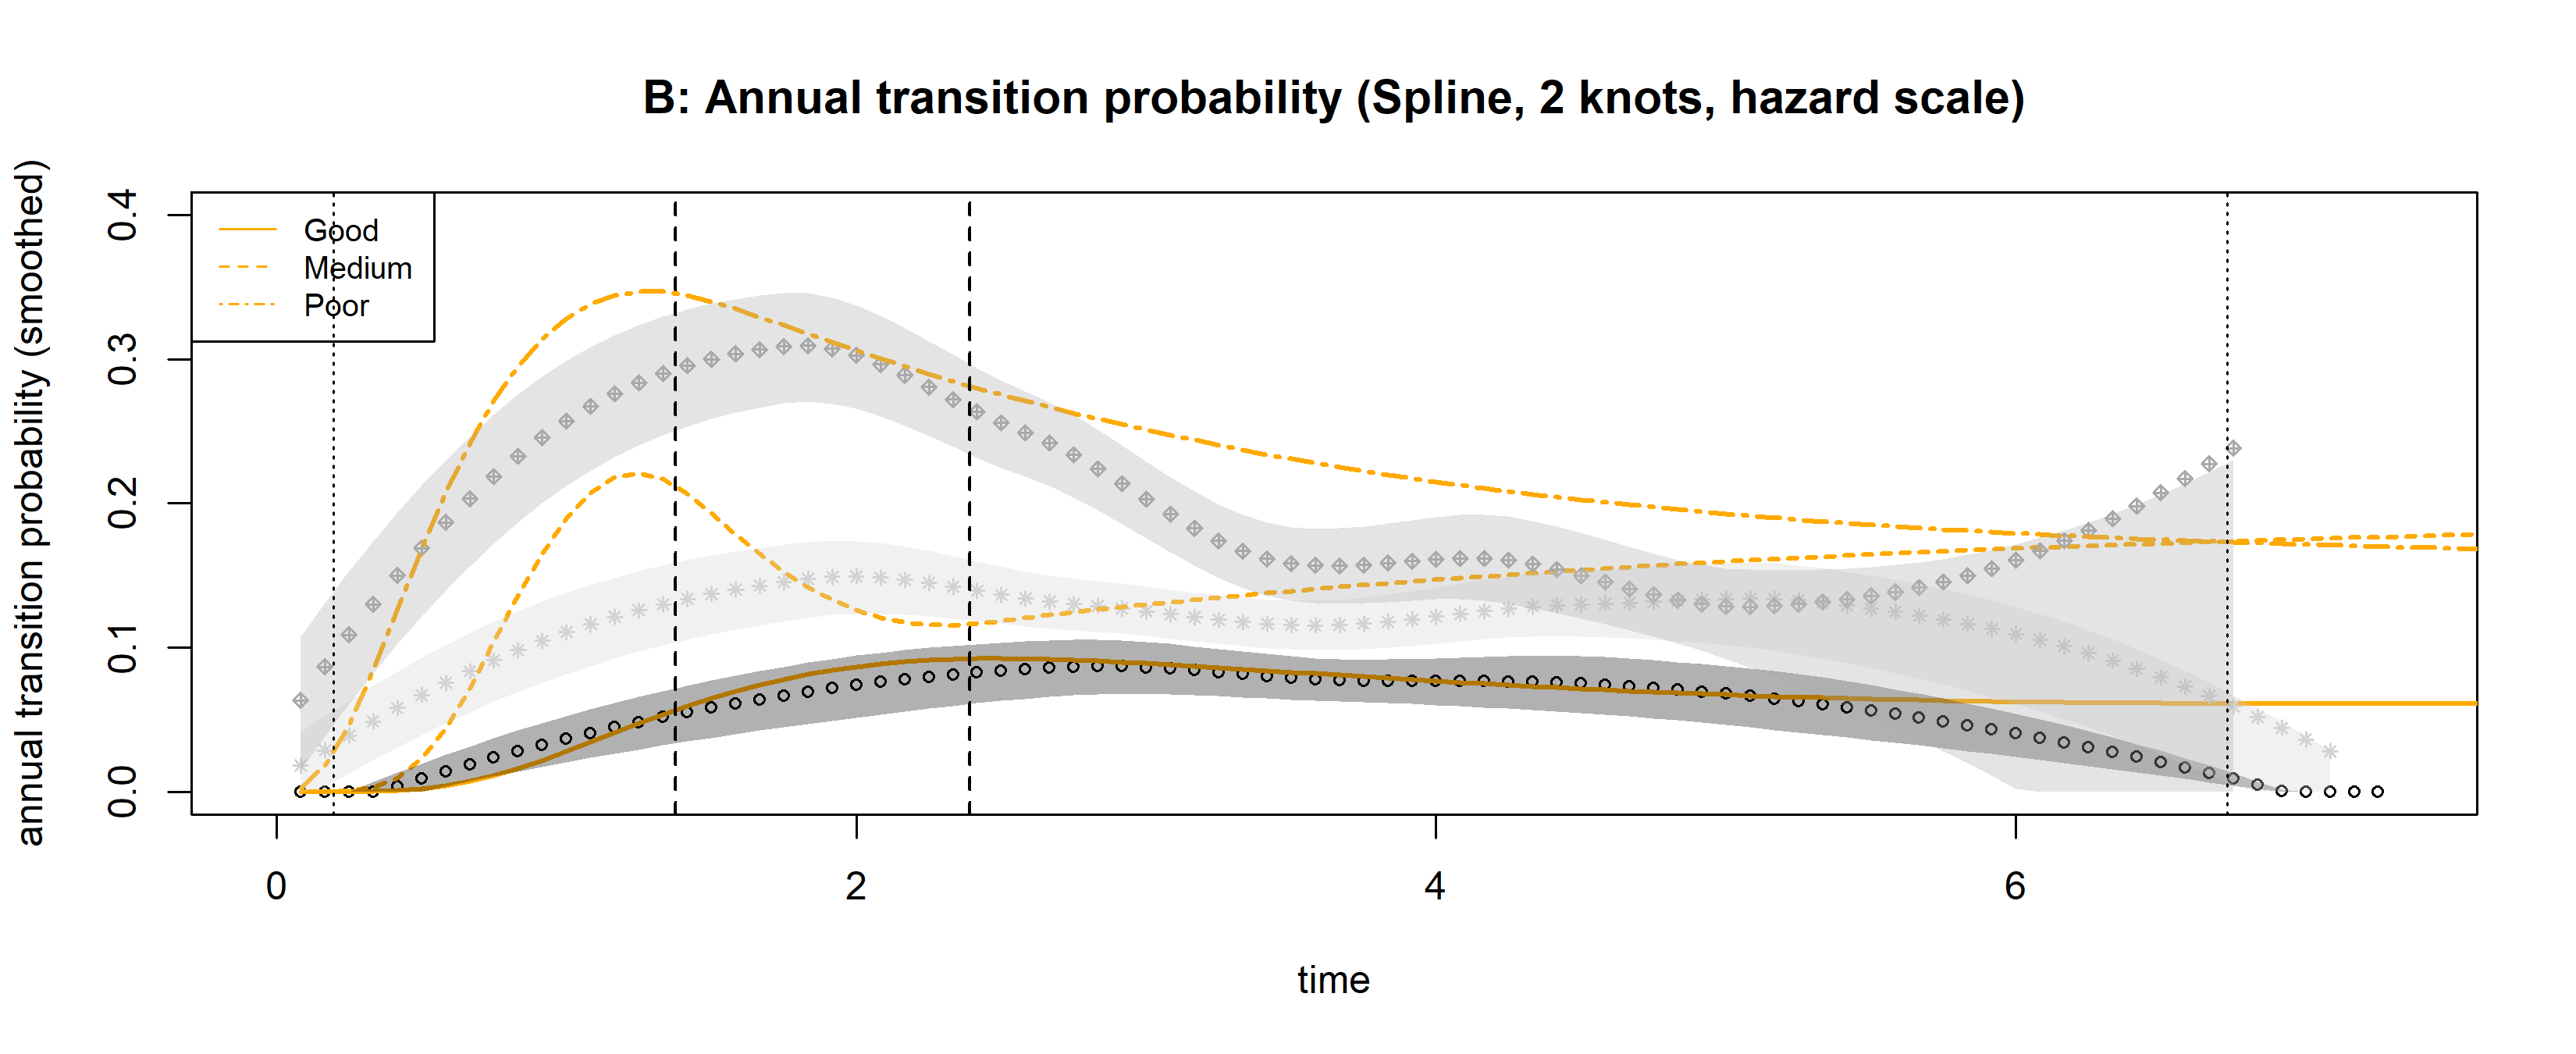
\includegraphics[height=0.3\textheight]{Images/spline_hazard2-2} \end{flushleft}

\begin{flushleft}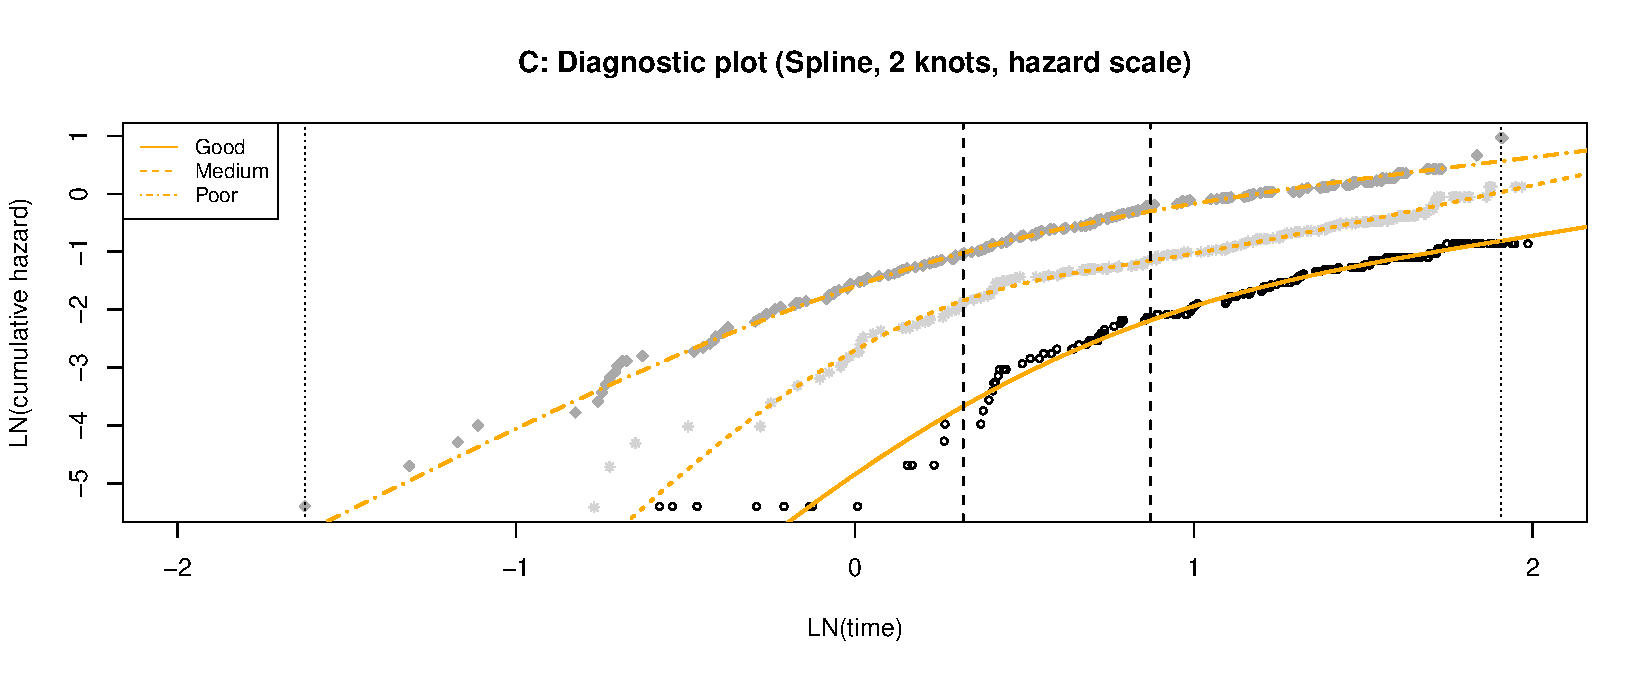
\includegraphics[height=0.3\textheight]{Images/spline_hazard2-3} \end{flushleft}

\subsection{Spline odds 1 knot}\label{spline-odds-1-knot}

\begin{flushleft}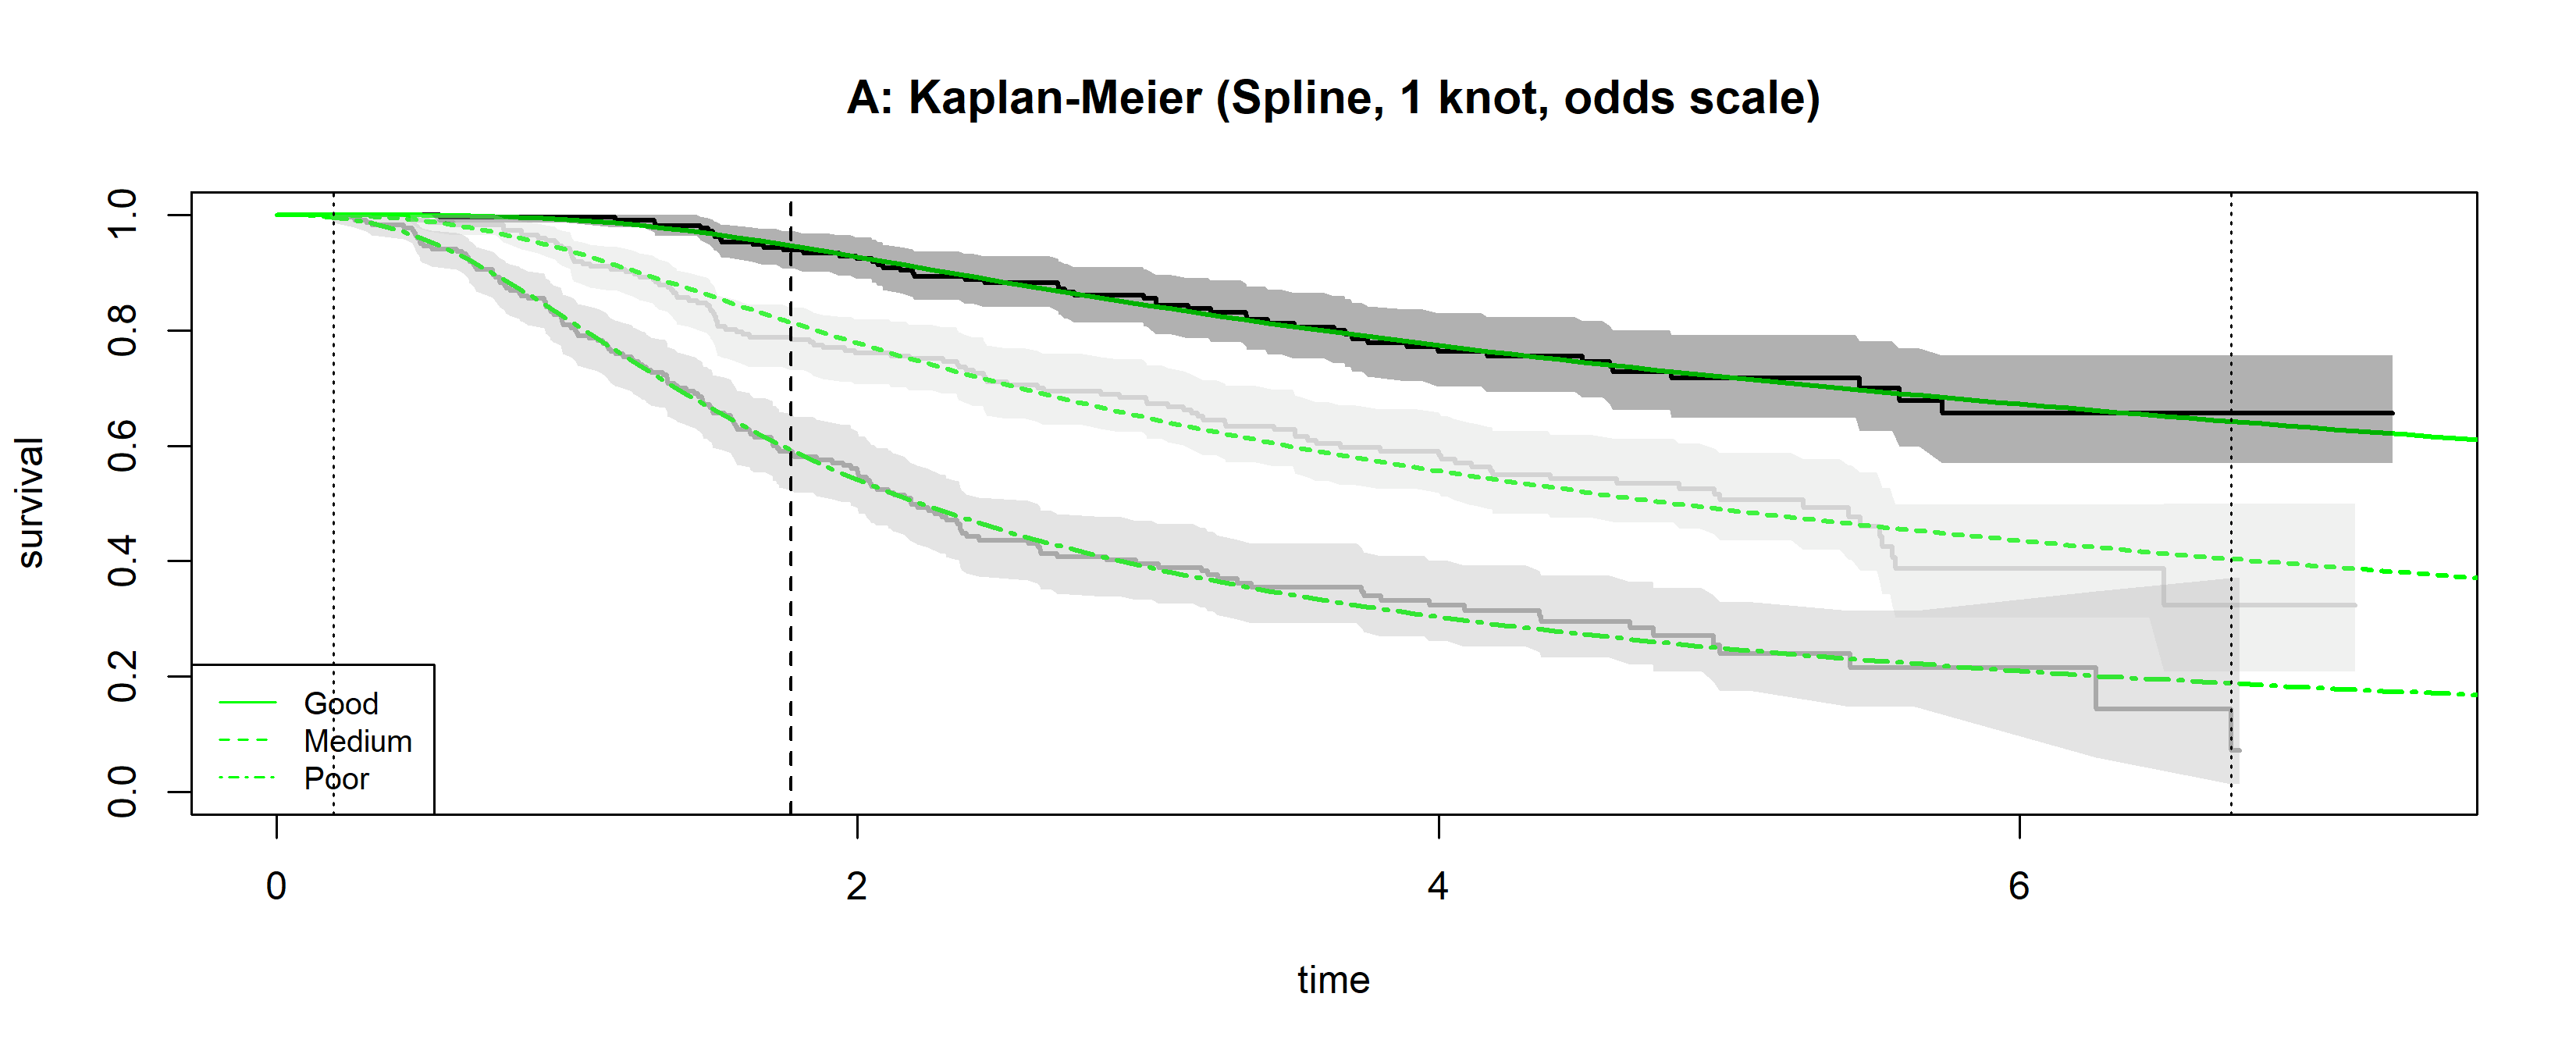
\includegraphics[height=0.3\textheight]{Images/spline_odds1-1} \end{flushleft}

\begin{flushleft}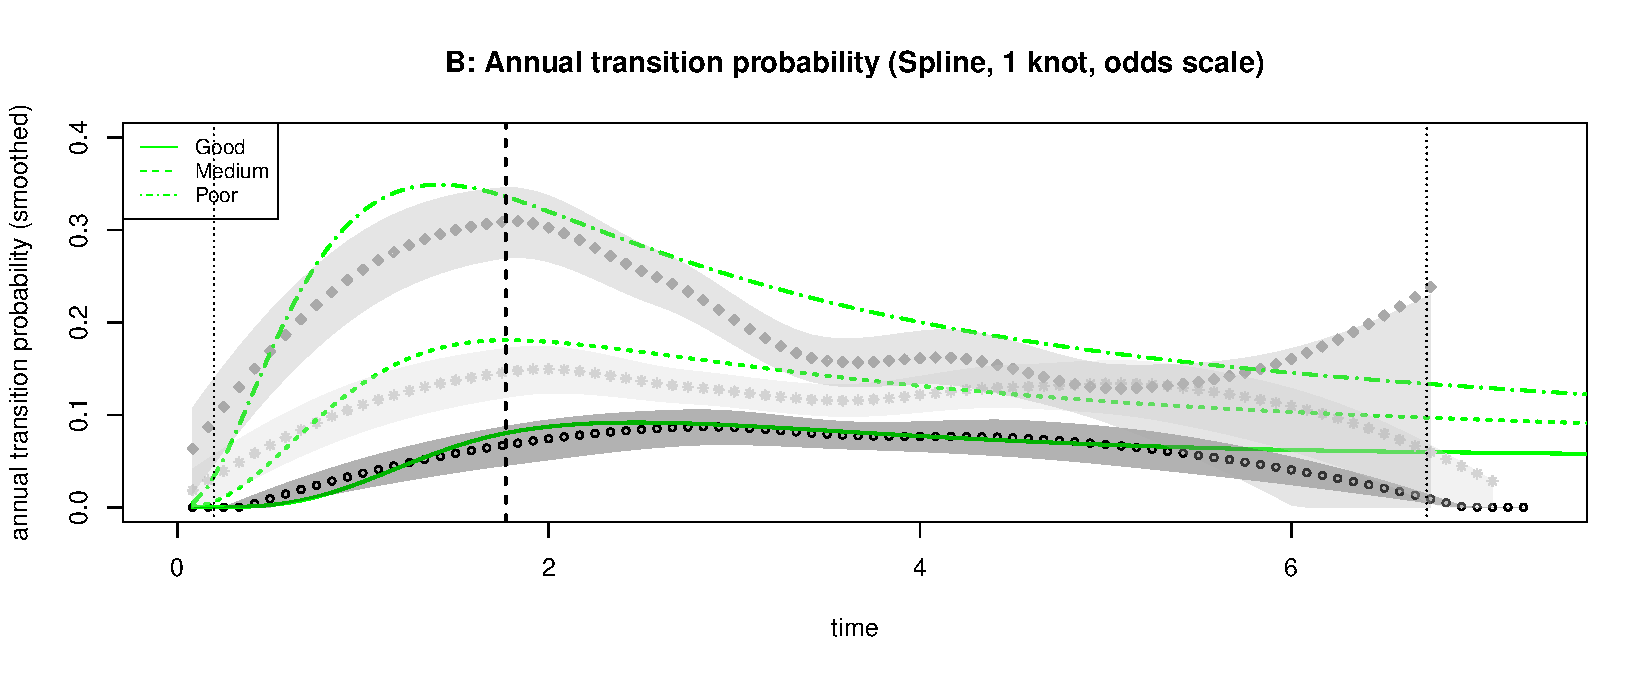
\includegraphics[height=0.3\textheight]{Images/spline_odds1-2} \end{flushleft}

\begin{flushleft}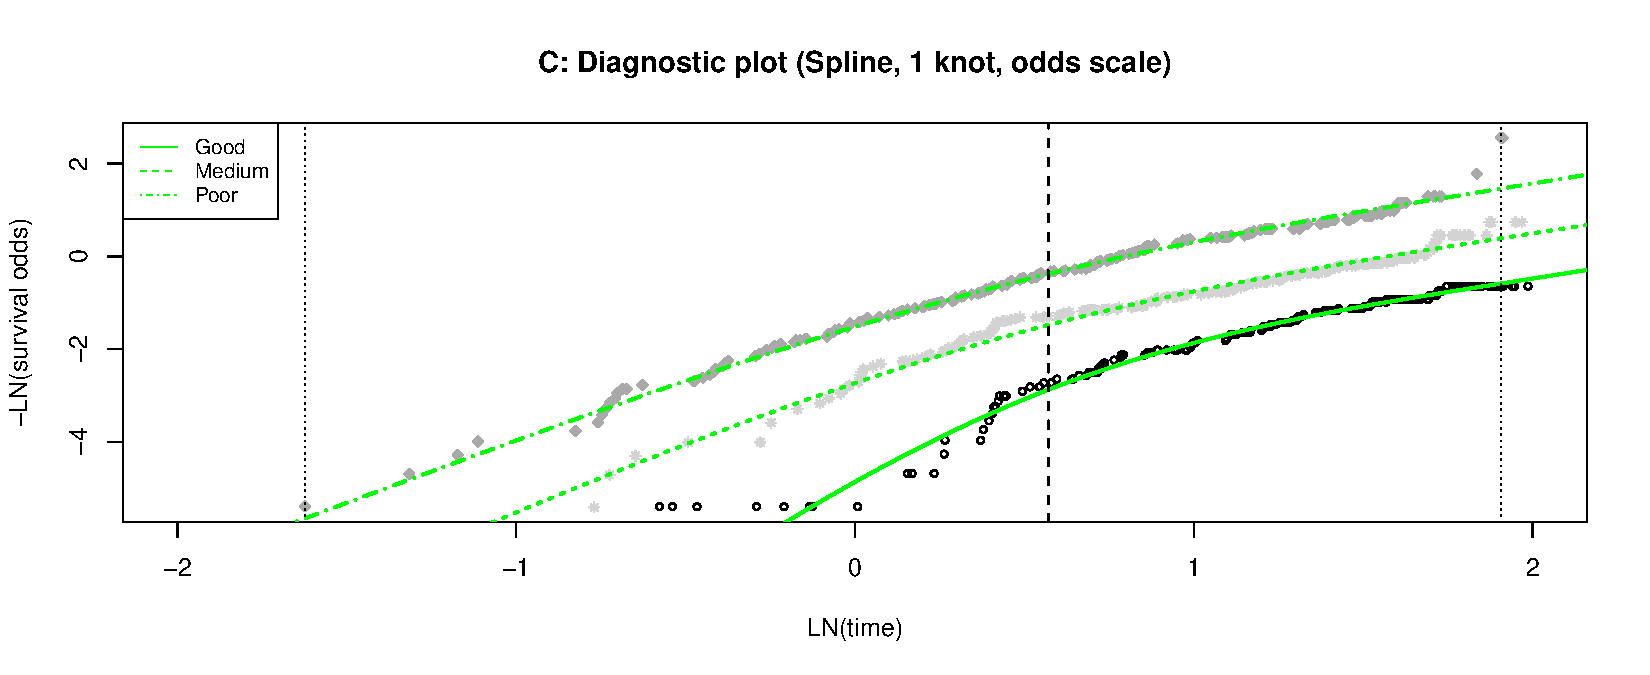
\includegraphics[height=0.3\textheight]{Images/spline_odds1-3} \end{flushleft}

\subsection{Spline odds 2 knots}\label{spline-odds-2-knots}

\begin{flushleft}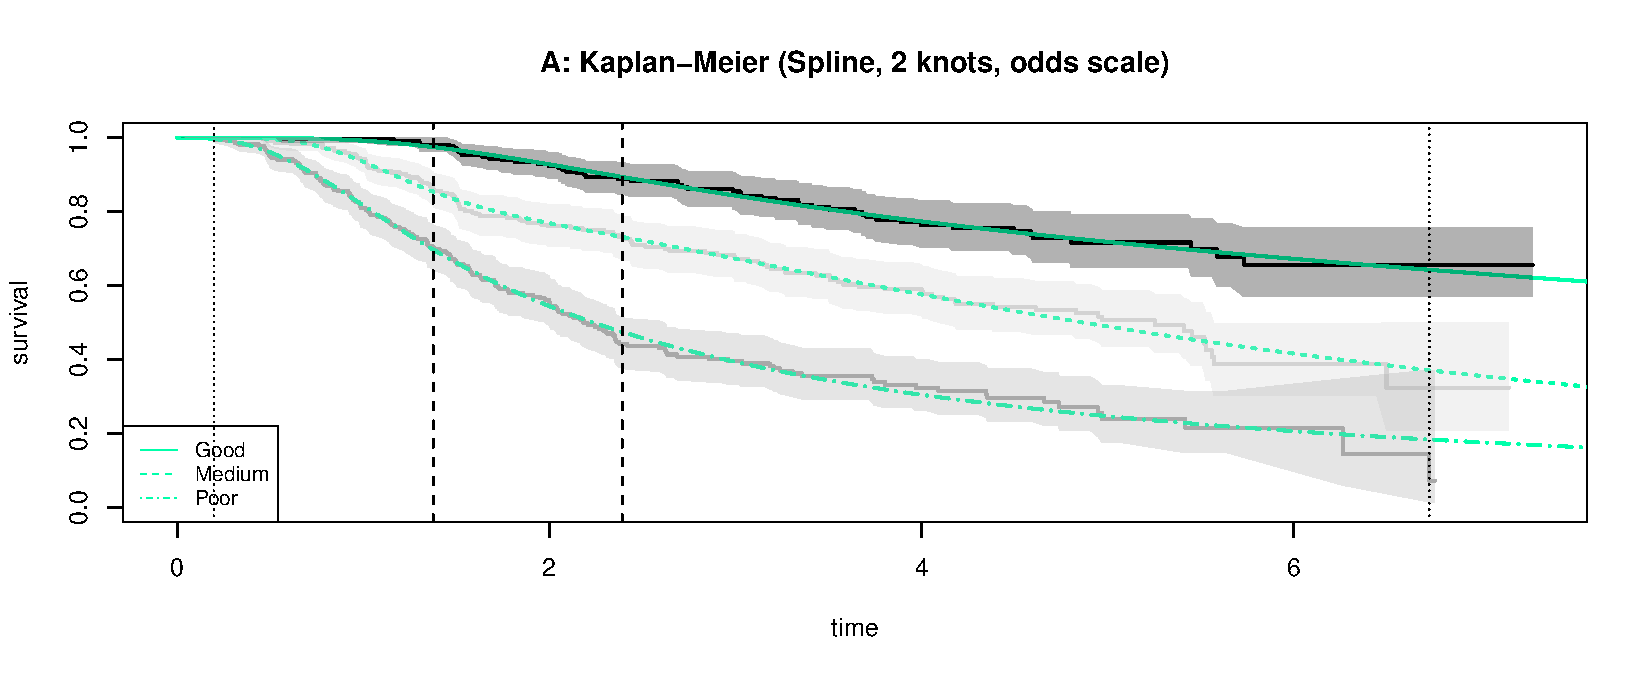
\includegraphics[height=0.3\textheight]{Images/spline_odds2-1} \end{flushleft}

\begin{flushleft}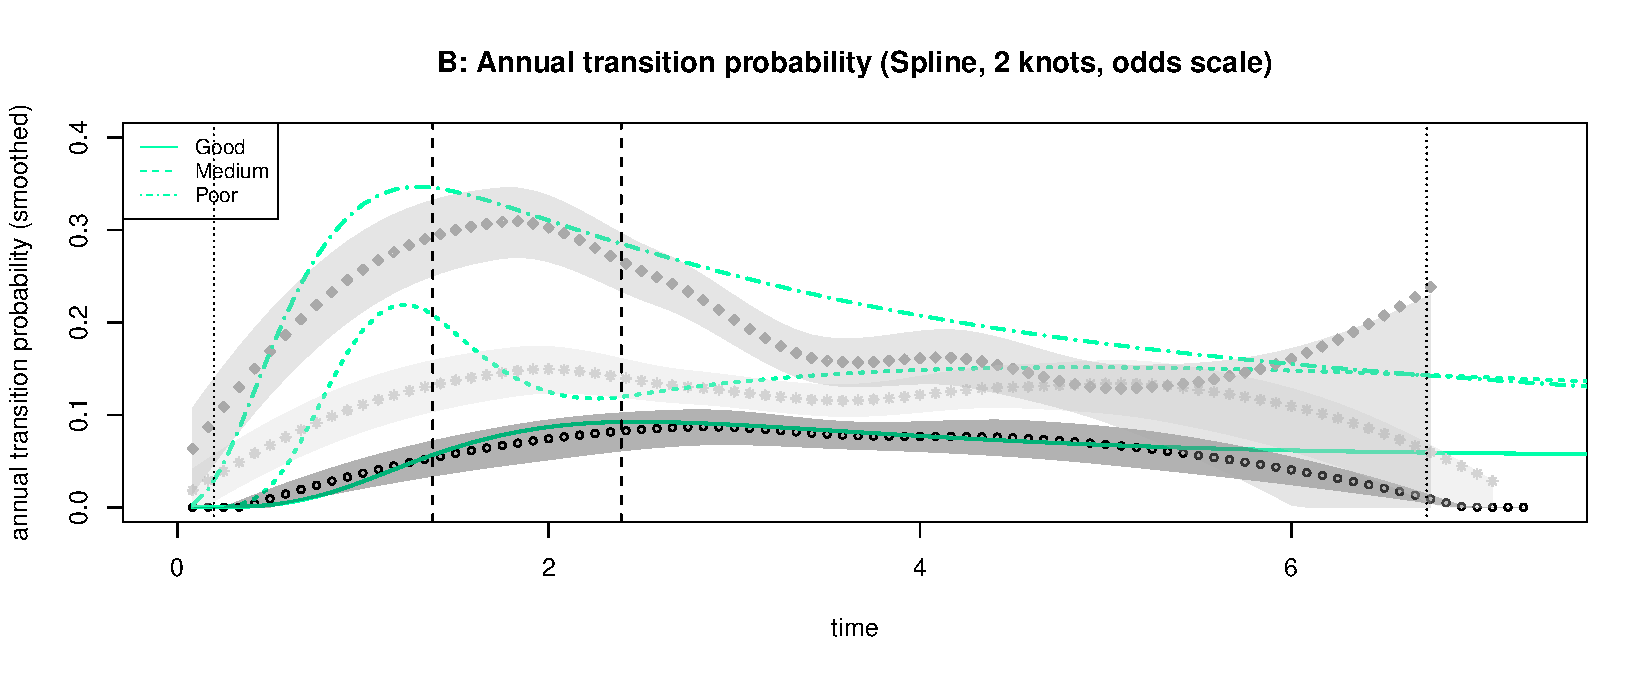
\includegraphics[height=0.3\textheight]{Images/spline_odds2-2} \end{flushleft}

\begin{flushleft}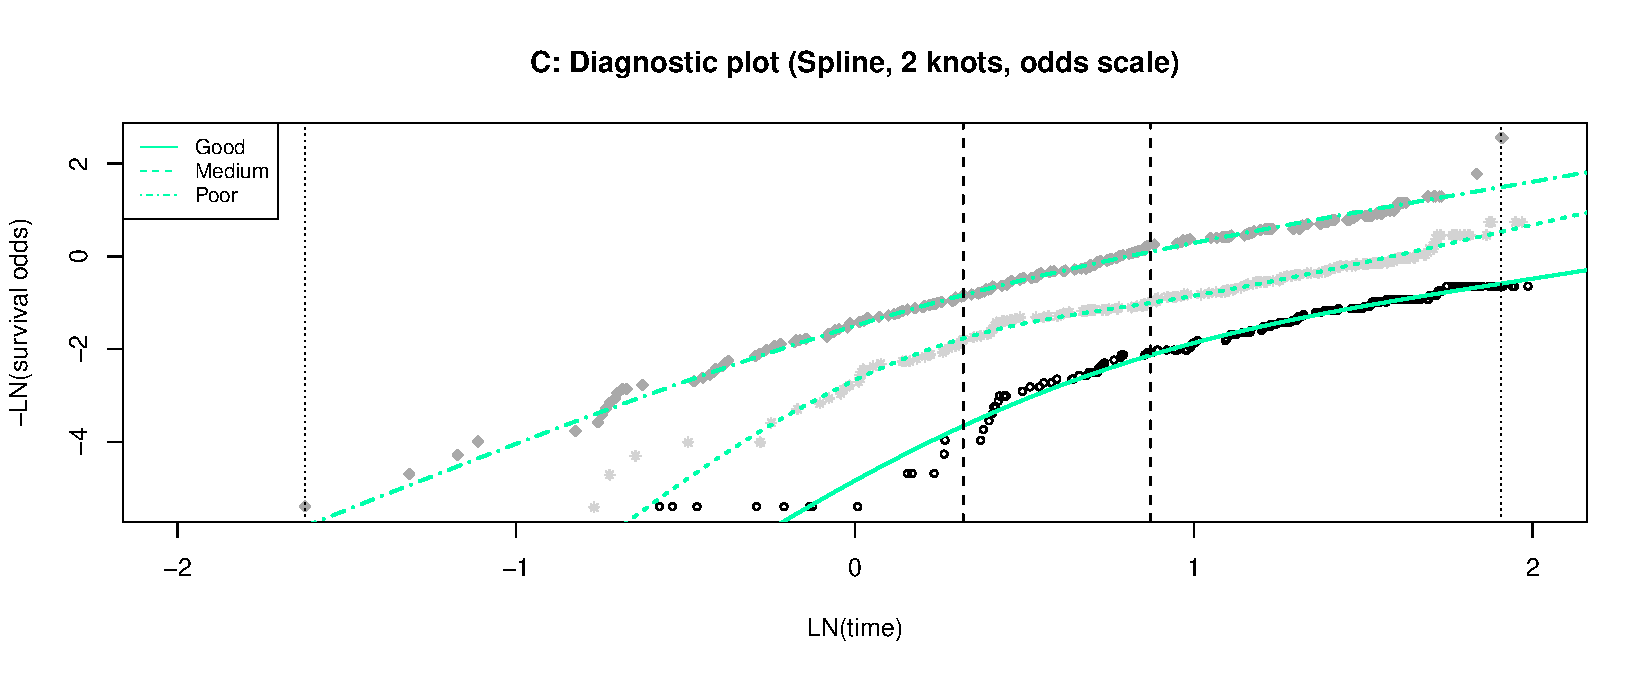
\includegraphics[height=0.3\textheight]{Images/spline_odds2-3} \end{flushleft}

\subsection{Spline normal 1 knot}\label{spline-normal-1-knot}

\begin{flushleft}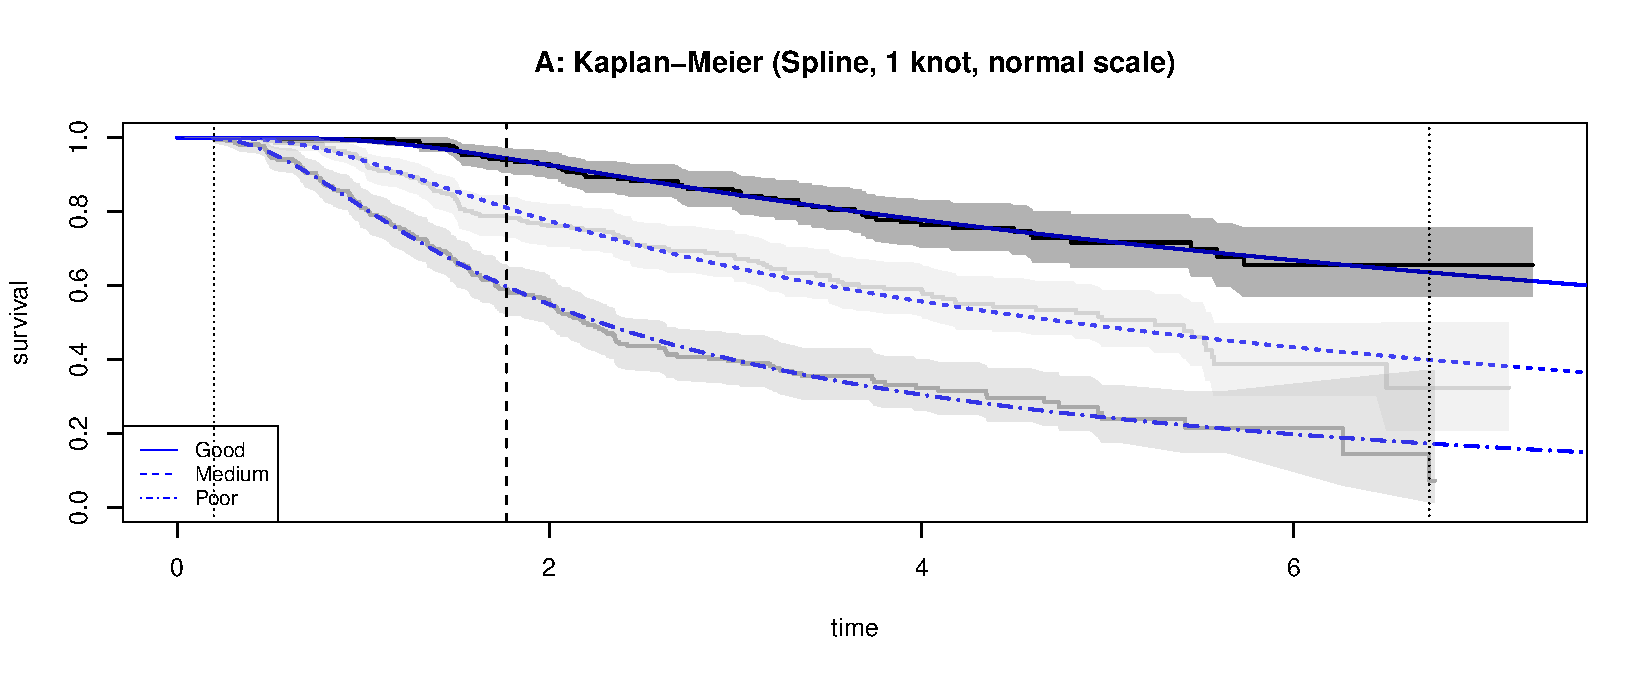
\includegraphics[height=0.3\textheight]{Images/spline_norm1-1} \end{flushleft}

\begin{flushleft}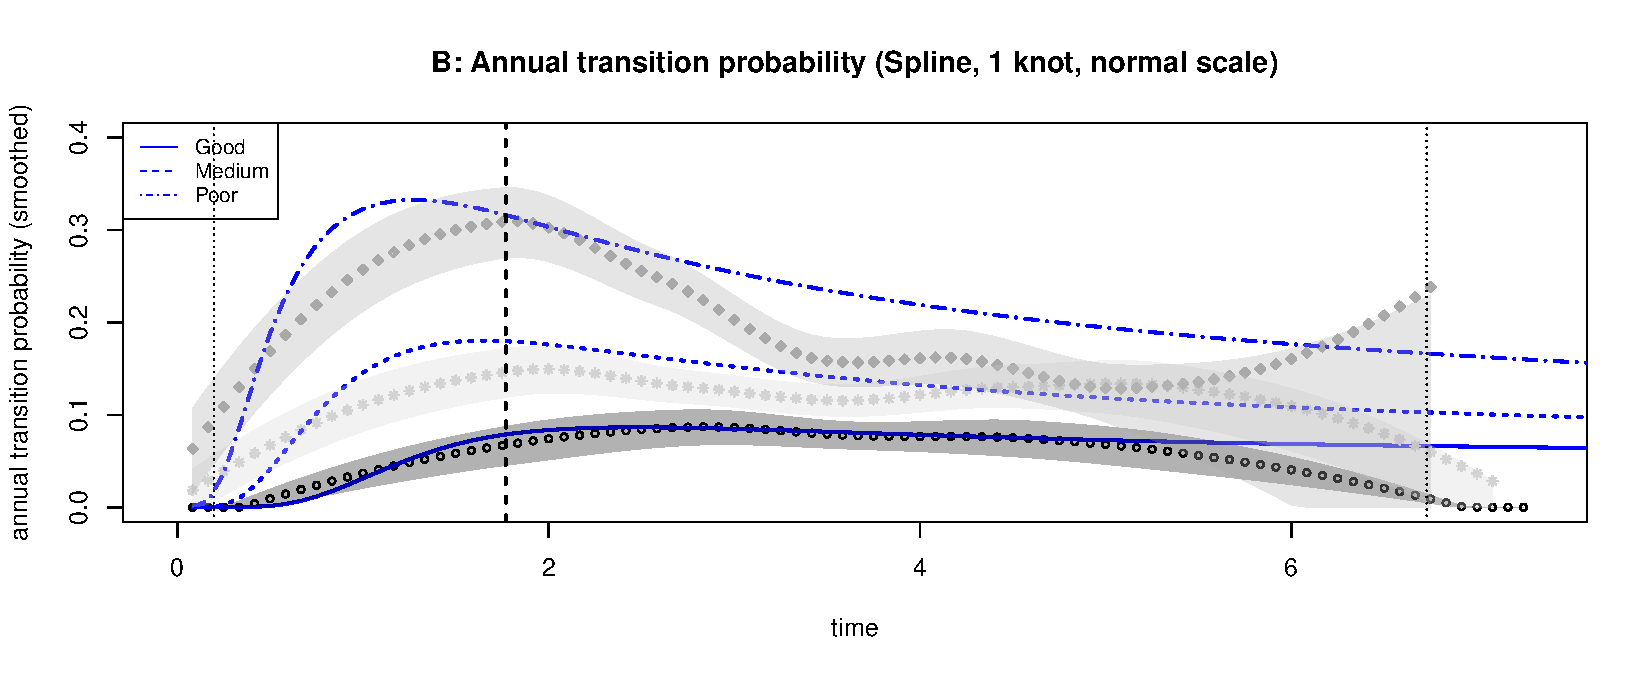
\includegraphics[height=0.3\textheight]{Images/spline_norm1-2} \end{flushleft}

\begin{flushleft}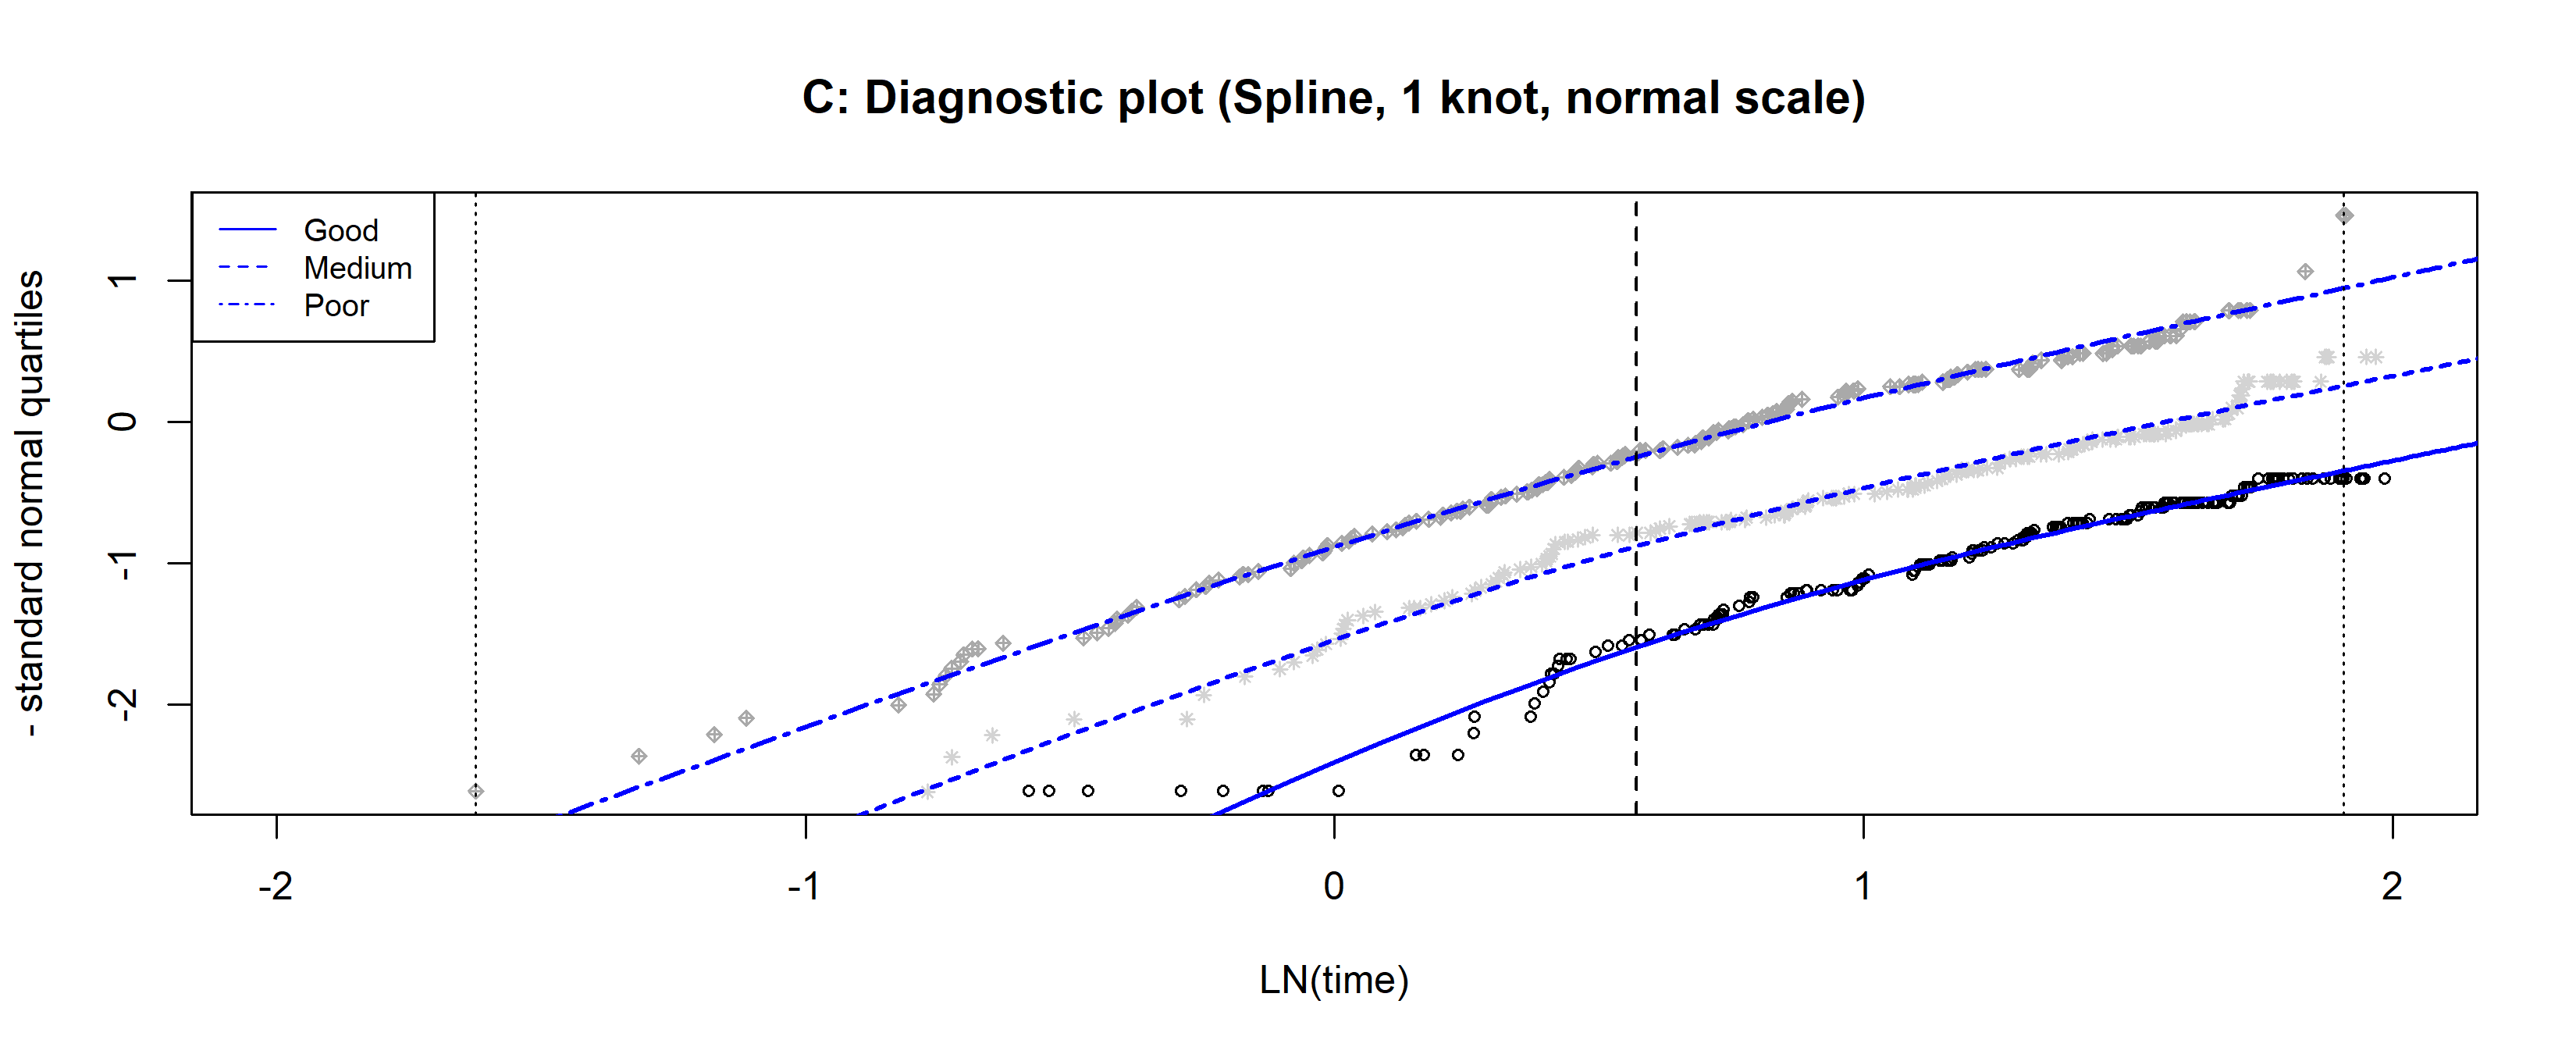
\includegraphics[height=0.3\textheight]{Images/spline_norm1-3} \end{flushleft}

\subsection{Spline normal 2 knots}\label{spline-normal-2-knots}

\begin{flushleft}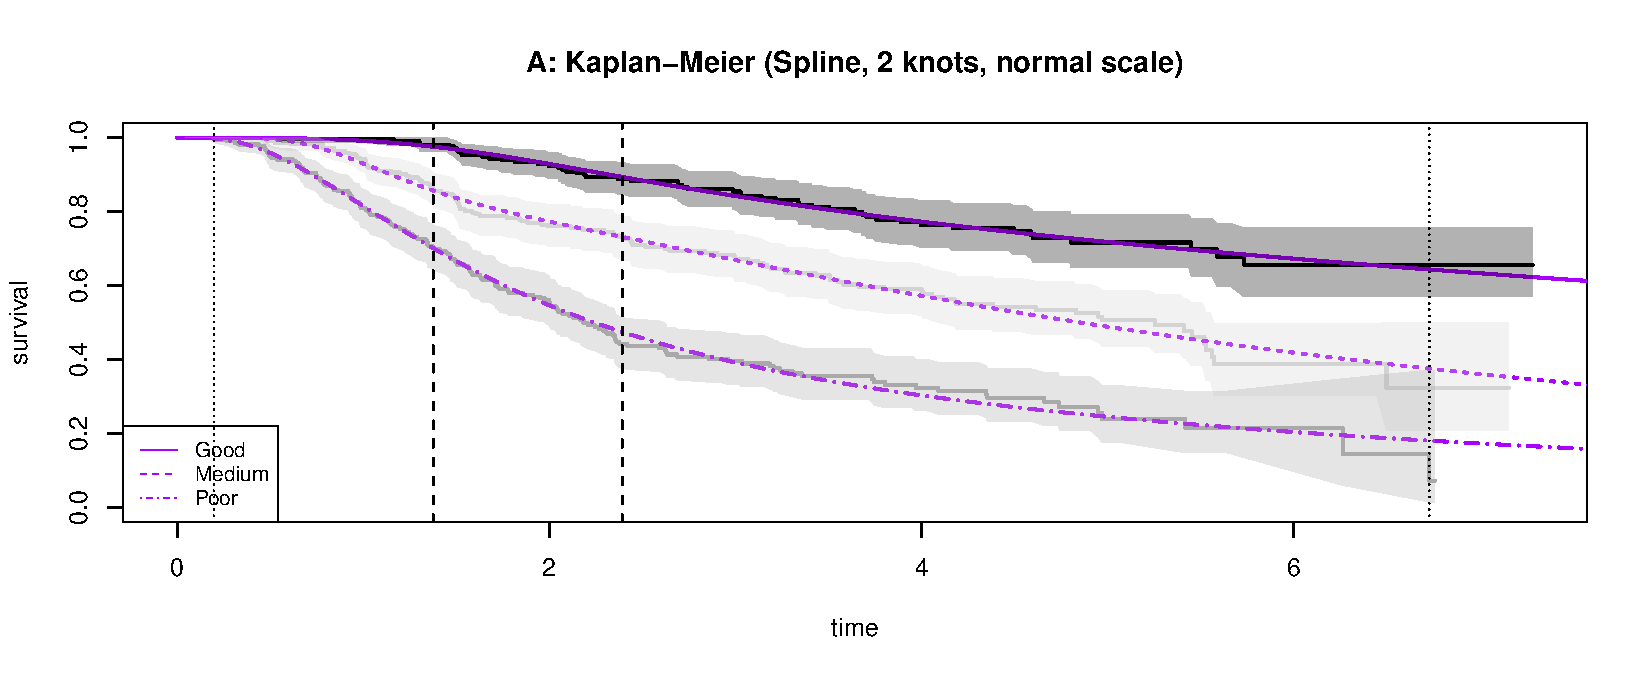
\includegraphics[height=0.3\textheight]{Images/spline_norm2-1} \end{flushleft}

\begin{flushleft}\includegraphics[height=0.3\textheight]{Images/spline_norm2-2} \end{flushleft}

\begin{flushleft}\includegraphics[height=0.3\textheight]{Images/spline_norm2-3} \end{flushleft}

\newpage

\section{Validity of long-term
extrapolation?}\label{validity-of-long-term-extrapolation}

What model(s) is/are more appropriate for long-term extrapolation?
Are/is the selected model(s) plausible in comparison with general
population mortality?

\subsection{Group Good}\label{group-good}

\begin{flushleft}\includegraphics[height=0.29\textheight]{Images/validate_extrapolation1-1} \end{flushleft}

\begin{flushleft}\includegraphics[height=0.29\textheight]{Images/validate_extrapolation1-2} \end{flushleft}

\resizebox{\linewidth}{!}{
\begin{tabular}{lrrrrrrrrrrrr}
\toprule
  & T= 0 & T= 1 & T= 2 & T= 3 & T= 4 & T= 5 & T= 10 & T= 15 & T= 20 & T= 25 & T= 30 & T= 35\\
\midrule
\cellcolor{gray!6}{1. Exponential} & \cellcolor{gray!6}{1} & \cellcolor{gray!6}{0.941} & \cellcolor{gray!6}{0.886} & \cellcolor{gray!6}{0.834} & \cellcolor{gray!6}{0.785} & \cellcolor{gray!6}{0.739} & \cellcolor{gray!6}{0.547} & \cellcolor{gray!6}{0.404} & \cellcolor{gray!6}{0.299} & \cellcolor{gray!6}{0.221} & \cellcolor{gray!6}{0.163} & \cellcolor{gray!6}{0.121}\\
2. Weibull & 1 & 0.978 & 0.932 & 0.870 & 0.797 & 0.719 & 0.345 & 0.122 & 0.033 & 0.007 & 0.001 & 0.000\\
\cellcolor{gray!6}{3. Gompertz} & \cellcolor{gray!6}{1} & \cellcolor{gray!6}{0.962} & \cellcolor{gray!6}{0.917} & \cellcolor{gray!6}{0.863} & \cellcolor{gray!6}{0.801} & \cellcolor{gray!6}{0.729} & \cellcolor{gray!6}{0.280} & \cellcolor{gray!6}{0.015} & \cellcolor{gray!6}{0.000} & \cellcolor{gray!6}{0.000} & \cellcolor{gray!6}{0.000} & \cellcolor{gray!6}{0.000}\\
4. Log-normal & 1 & 0.986 & 0.933 & 0.861 & 0.785 & 0.713 & 0.441 & 0.287 & 0.196 & 0.139 & 0.102 & 0.076\\
\cellcolor{gray!6}{5. Log-logistic} & \cellcolor{gray!6}{1} & \cellcolor{gray!6}{0.980} & \cellcolor{gray!6}{0.932} & \cellcolor{gray!6}{0.865} & \cellcolor{gray!6}{0.789} & \cellcolor{gray!6}{0.712} & \cellcolor{gray!6}{0.403} & \cellcolor{gray!6}{0.240} & \cellcolor{gray!6}{0.156} & \cellcolor{gray!6}{0.108} & \cellcolor{gray!6}{0.080} & \cellcolor{gray!6}{0.061}\\
6. Gamma & 1 & 0.982 & 0.935 & 0.869 & 0.793 & 0.714 & 0.367 & 0.165 & 0.069 & 0.027 & 0.011 & 0.004\\
\cellcolor{gray!6}{7. Generalised Gamma} & \cellcolor{gray!6}{1} & \cellcolor{gray!6}{0.991} & \cellcolor{gray!6}{0.928} & \cellcolor{gray!6}{0.849} & \cellcolor{gray!6}{0.778} & \cellcolor{gray!6}{0.717} & \cellcolor{gray!6}{0.526} & \cellcolor{gray!6}{0.425} & \cellcolor{gray!6}{0.362} & \cellcolor{gray!6}{0.319} & \cellcolor{gray!6}{0.286} & \cellcolor{gray!6}{0.261}\\
8. Spline 1 knot hazard & 1 & 0.992 & 0.927 & 0.843 & 0.774 & 0.719 & 0.521 & 0.381 & 0.279 & 0.205 & 0.151 & 0.111\\
\cellcolor{gray!6}{9. Spline 2 knots hazard} & \cellcolor{gray!6}{1} & \cellcolor{gray!6}{0.992} & \cellcolor{gray!6}{0.928} & \cellcolor{gray!6}{0.843} & \cellcolor{gray!6}{0.774} & \cellcolor{gray!6}{0.719} & \cellcolor{gray!6}{0.523} & \cellcolor{gray!6}{0.384} & \cellcolor{gray!6}{0.283} & \cellcolor{gray!6}{0.210} & \cellcolor{gray!6}{0.156} & \cellcolor{gray!6}{0.116}\\
10. Spline 1 knot odds & 1 & 0.992 & 0.927 & 0.843 & 0.774 & 0.718 & 0.532 & 0.415 & 0.338 & 0.283 & 0.242 & 0.211\\
\cellcolor{gray!6}{11. Spline 2 knots odds} & \cellcolor{gray!6}{1} & \cellcolor{gray!6}{0.992} & \cellcolor{gray!6}{0.928} & \cellcolor{gray!6}{0.843} & \cellcolor{gray!6}{0.774} & \cellcolor{gray!6}{0.718} & \cellcolor{gray!6}{0.533} & \cellcolor{gray!6}{0.418} & \cellcolor{gray!6}{0.340} & \cellcolor{gray!6}{0.285} & \cellcolor{gray!6}{0.245} & \cellcolor{gray!6}{0.213}\\
12. Spline 1 knot normal & 1 & 0.992 & 0.926 & 0.847 & 0.778 & 0.719 & 0.515 & 0.391 & 0.308 & 0.250 & 0.207 & 0.174\\
\cellcolor{gray!6}{13. Spline 2 knots normal} & \cellcolor{gray!6}{1} & \cellcolor{gray!6}{0.992} & \cellcolor{gray!6}{0.929} & \cellcolor{gray!6}{0.842} & \cellcolor{gray!6}{0.773} & \cellcolor{gray!6}{0.718} & \cellcolor{gray!6}{0.538} & \cellcolor{gray!6}{0.426} & \cellcolor{gray!6}{0.350} & \cellcolor{gray!6}{0.295} & \cellcolor{gray!6}{0.253} & \cellcolor{gray!6}{0.220}\\
\bottomrule
\end{tabular}}

\begin{flushleft}\includegraphics[height=0.29\textheight]{Images/validate_extrapolation1-3} \end{flushleft}

\begin{flushleft}\includegraphics[height=0.29\textheight]{Images/validate_extrapolation1-4} \end{flushleft}

\begin{tabular}{lrrrrr}
\toprule
  & Min & Q1 & Median & Q3 & Max\\
\midrule
\cellcolor{gray!6}{1. Exponential} & \cellcolor{gray!6}{0.0585969} & \cellcolor{gray!6}{0.0585969} & \cellcolor{gray!6}{0.0585969} & \cellcolor{gray!6}{0.0585969} & \cellcolor{gray!6}{0.0585969}\\
2. Weibull & 0.0039603 & 0.1641779 & 0.2507544 & 0.3170901 & 0.3714738\\
\cellcolor{gray!6}{3. Gompertz} & \cellcolor{gray!6}{0.0342601} & \cellcolor{gray!6}{0.1256322} & \cellcolor{gray!6}{0.4037134} & \cellcolor{gray!6}{0.8634656} & \cellcolor{gray!6}{1.0000000}\\
4. Log-normal & 0.0000121 & 0.0563972 & 0.0670524 & 0.0819079 & 0.0936091\\
\cellcolor{gray!6}{5. Log-logistic} & \cellcolor{gray!6}{0.0022936} & \cellcolor{gray!6}{0.0533146} & \cellcolor{gray!6}{0.0700441} & \cellcolor{gray!6}{0.0935993} & \cellcolor{gray!6}{0.1092616}\\
6. Gamma & 0.0014181 & 0.1390361 & 0.1644882 & 0.1750195 & 0.1807519\\
\cellcolor{gray!6}{7. Generalised Gamma} & \cellcolor{gray!6}{0.0000000} & \cellcolor{gray!6}{0.0191123} & \cellcolor{gray!6}{0.0269247} & \cellcolor{gray!6}{0.0452063} & \cellcolor{gray!6}{0.0862100}\\
8. Spline 1 knot hazard & 0.0000002 & 0.0592140 & 0.0598953 & 0.0610195 & 0.0916043\\
\cellcolor{gray!6}{9. Spline 2 knots hazard} & \cellcolor{gray!6}{0.0000002} & \cellcolor{gray!6}{0.0576502} & \cellcolor{gray!6}{0.0585313} & \cellcolor{gray!6}{0.0599923} & \cellcolor{gray!6}{0.0923962}\\
10. Spline 1 knot odds & 0.0000002 & 0.0281269 & 0.0363823 & 0.0502992 & 0.0917044\\
\cellcolor{gray!6}{11. Spline 2 knots odds} & \cellcolor{gray!6}{0.0000002} & \cellcolor{gray!6}{0.0278516} & \cellcolor{gray!6}{0.0359503} & \cellcolor{gray!6}{0.0497462} & \cellcolor{gray!6}{0.0924439}\\
12. Spline 1 knot normal & 0.0000000 & 0.0345970 & 0.0424046 & 0.0560095 & 0.0865141\\
\cellcolor{gray!6}{13. Spline 2 knots normal} & \cellcolor{gray!6}{0.0000006} & \cellcolor{gray!6}{0.0281480} & \cellcolor{gray!6}{0.0348987} & \cellcolor{gray!6}{0.0473455} & \cellcolor{gray!6}{0.0953359}\\
\bottomrule
\end{tabular}

\begin{flushleft}\includegraphics[height=0.29\textheight]{Images/validate_extrapolation1-5} \end{flushleft}

\begin{flushleft}\includegraphics[height=0.29\textheight]{Images/validate_extrapolation1-6} \end{flushleft}

\newpage

\subsection{Group Medium}\label{group-medium}

\begin{flushleft}\includegraphics[height=0.29\textheight]{Images/validate_extrapolation2-1} \end{flushleft}

\begin{flushleft}\includegraphics[height=0.29\textheight]{Images/validate_extrapolation2-2} \end{flushleft}

\resizebox{\linewidth}{!}{
\begin{tabular}{lrrrrrrrrrrrr}
\toprule
  & T= 0 & T= 1 & T= 2 & T= 3 & T= 4 & T= 5 & T= 10 & T= 15 & T= 20 & T= 25 & T= 30 & T= 35\\
\midrule
\cellcolor{gray!6}{1. Exponential} & \cellcolor{gray!6}{1} & \cellcolor{gray!6}{0.872} & \cellcolor{gray!6}{0.761} & \cellcolor{gray!6}{0.663} & \cellcolor{gray!6}{0.578} & \cellcolor{gray!6}{0.505} & \cellcolor{gray!6}{0.255} & \cellcolor{gray!6}{0.128} & \cellcolor{gray!6}{0.065} & \cellcolor{gray!6}{0.033} & \cellcolor{gray!6}{0.016} & \cellcolor{gray!6}{0.008}\\
2. Weibull & 1 & 0.923 & 0.811 & 0.693 & 0.578 & 0.474 & 0.141 & 0.032 & 0.006 & 0.001 & 0.000 & 0.000\\
\cellcolor{gray!6}{3. Gompertz} & \cellcolor{gray!6}{1} & \cellcolor{gray!6}{0.898} & \cellcolor{gray!6}{0.794} & \cellcolor{gray!6}{0.689} & \cellcolor{gray!6}{0.586} & \cellcolor{gray!6}{0.486} & \cellcolor{gray!6}{0.117} & \cellcolor{gray!6}{0.007} & \cellcolor{gray!6}{0.000} & \cellcolor{gray!6}{0.000} & \cellcolor{gray!6}{0.000} & \cellcolor{gray!6}{0.000}\\
4. Log-normal & 1 & 0.935 & 0.797 & 0.668 & 0.560 & 0.473 & 0.228 & 0.126 & 0.077 & 0.050 & 0.034 & 0.024\\
\cellcolor{gray!6}{5. Log-logistic} & \cellcolor{gray!6}{1} & \cellcolor{gray!6}{0.927} & \cellcolor{gray!6}{0.801} & \cellcolor{gray!6}{0.673} & \cellcolor{gray!6}{0.561} & \cellcolor{gray!6}{0.468} & \cellcolor{gray!6}{0.218} & \cellcolor{gray!6}{0.124} & \cellcolor{gray!6}{0.081} & \cellcolor{gray!6}{0.057} & \cellcolor{gray!6}{0.043} & \cellcolor{gray!6}{0.034}\\
6. Gamma & 1 & 0.930 & 0.813 & 0.689 & 0.572 & 0.469 & 0.154 & 0.045 & 0.013 & 0.003 & 0.001 & 0.000\\
\cellcolor{gray!6}{7. Generalised Gamma} & \cellcolor{gray!6}{1} & \cellcolor{gray!6}{0.937} & \cellcolor{gray!6}{0.774} & \cellcolor{gray!6}{0.648} & \cellcolor{gray!6}{0.556} & \cellcolor{gray!6}{0.488} & \cellcolor{gray!6}{0.310} & \cellcolor{gray!6}{0.232} & \cellcolor{gray!6}{0.187} & \cellcolor{gray!6}{0.158} & \cellcolor{gray!6}{0.138} & \cellcolor{gray!6}{0.122}\\
8. Spline 1 knot hazard & 1 & 0.939 & 0.782 & 0.652 & 0.558 & 0.486 & 0.265 & 0.150 & 0.087 & 0.052 & 0.031 & 0.019\\
\cellcolor{gray!6}{9. Spline 2 knots hazard} & \cellcolor{gray!6}{1} & \cellcolor{gray!6}{0.935} & \cellcolor{gray!6}{0.766} & \cellcolor{gray!6}{0.673} & \cellcolor{gray!6}{0.579} & \cellcolor{gray!6}{0.490} & \cellcolor{gray!6}{0.184} & \cellcolor{gray!6}{0.061} & \cellcolor{gray!6}{0.018} & \cellcolor{gray!6}{0.005} & \cellcolor{gray!6}{0.001} & \cellcolor{gray!6}{0.000}\\
10. Spline 1 knot odds & 1 & 0.939 & 0.778 & 0.648 & 0.556 & 0.489 & 0.301 & 0.213 & 0.162 & 0.131 & 0.109 & 0.093\\
\cellcolor{gray!6}{11. Spline 2 knots odds} & \cellcolor{gray!6}{1} & \cellcolor{gray!6}{0.935} & \cellcolor{gray!6}{0.769} & \cellcolor{gray!6}{0.673} & \cellcolor{gray!6}{0.576} & \cellcolor{gray!6}{0.489} & \cellcolor{gray!6}{0.235} & \cellcolor{gray!6}{0.136} & \cellcolor{gray!6}{0.089} & \cellcolor{gray!6}{0.063} & \cellcolor{gray!6}{0.048} & \cellcolor{gray!6}{0.037}\\
12. Spline 1 knot normal & 1 & 0.938 & 0.775 & 0.648 & 0.557 & 0.488 & 0.290 & 0.195 & 0.141 & 0.107 & 0.084 & 0.067\\
\cellcolor{gray!6}{13. Spline 2 knots normal} & \cellcolor{gray!6}{1} & \cellcolor{gray!6}{0.930} & \cellcolor{gray!6}{0.773} & \cellcolor{gray!6}{0.669} & \cellcolor{gray!6}{0.572} & \cellcolor{gray!6}{0.489} & \cellcolor{gray!6}{0.240} & \cellcolor{gray!6}{0.135} & \cellcolor{gray!6}{0.083} & \cellcolor{gray!6}{0.054} & \cellcolor{gray!6}{0.037} & \cellcolor{gray!6}{0.026}\\
\bottomrule
\end{tabular}}

\begin{flushleft}\includegraphics[height=0.29\textheight]{Images/validate_extrapolation2-3} \end{flushleft}

\begin{flushleft}\includegraphics[height=0.29\textheight]{Images/validate_extrapolation2-4} \end{flushleft}

\begin{tabular}{lrrrrr}
\toprule
  & Min & Q1 & Median & Q3 & Max\\
\midrule
\cellcolor{gray!6}{1. Exponential} & \cellcolor{gray!6}{0.1278820} & \cellcolor{gray!6}{0.1278820} & \cellcolor{gray!6}{0.1278820} & \cellcolor{gray!6}{0.1278820} & \cellcolor{gray!6}{0.1278820}\\
2. Weibull & 0.0298491 & 0.2382194 & 0.2998675 & 0.3413164 & 0.3730304\\
\cellcolor{gray!6}{3. Gompertz} & \cellcolor{gray!6}{0.0960264} & \cellcolor{gray!6}{0.2326209} & \cellcolor{gray!6}{0.5026105} & \cellcolor{gray!6}{0.8415103} & \cellcolor{gray!6}{1.0000000}\\
4. Log-normal & 0.0004751 & 0.0692201 & 0.0864990 & 0.1175437 & 0.1630482\\
\cellcolor{gray!6}{5. Log-logistic} & \cellcolor{gray!6}{0.0150627} & \cellcolor{gray!6}{0.0512119} & \cellcolor{gray!6}{0.0722192} & \cellcolor{gray!6}{0.1148301} & \cellcolor{gray!6}{0.1673124}\\
6. Gamma & 0.0159374 & 0.2105278 & 0.2273428 & 0.2338793 & 0.2373538\\
\cellcolor{gray!6}{7. Generalised Gamma} & \cellcolor{gray!6}{0.0000000} & \cellcolor{gray!6}{0.0249765} & \cellcolor{gray!6}{0.0361491} & \cellcolor{gray!6}{0.0643696} & \cellcolor{gray!6}{0.1783037}\\
8. Spline 1 knot hazard & 0.0005533 & 0.0961200 & 0.1007177 & 0.1087714 & 0.1767370\\
\cellcolor{gray!6}{9. Spline 2 knots hazard} & \cellcolor{gray!6}{0.0000006} & \cellcolor{gray!6}{0.1921569} & \cellcolor{gray!6}{0.2213494} & \cellcolor{gray!6}{0.2415978} & \cellcolor{gray!6}{0.2568265}\\
10. Spline 1 knot odds & 0.0004610 & 0.0331955 & 0.0461415 & 0.0743721 & 0.1809477\\
\cellcolor{gray!6}{11. Spline 2 knots odds} & \cellcolor{gray!6}{0.0000004} & \cellcolor{gray!6}{0.0500917} & \cellcolor{gray!6}{0.0706148} & \cellcolor{gray!6}{0.1135216} & \cellcolor{gray!6}{0.2192447}\\
12. Spline 1 knot normal & 0.0000012 & 0.0444894 & 0.0569700 & 0.0823605 & 0.1804334\\
\cellcolor{gray!6}{13. Spline 2 knots normal} & \cellcolor{gray!6}{0.0000000} & \cellcolor{gray!6}{0.0682231} & \cellcolor{gray!6}{0.0852159} & \cellcolor{gray!6}{0.1164045} & \cellcolor{gray!6}{0.2005479}\\
\bottomrule
\end{tabular}

\begin{flushleft}\includegraphics[height=0.29\textheight]{Images/validate_extrapolation2-5} \end{flushleft}

\begin{flushleft}\includegraphics[height=0.29\textheight]{Images/validate_extrapolation2-6} \end{flushleft}

\newpage

\subsection{Group Poor}\label{group-poor}

\begin{flushleft}\includegraphics[height=0.29\textheight]{Images/validate_extrapolation3-1} \end{flushleft}

\begin{flushleft}\includegraphics[height=0.29\textheight]{Images/validate_extrapolation3-2} \end{flushleft}

\resizebox{\linewidth}{!}{
\begin{tabular}{lrrrrrrrrrrrr}
\toprule
  & T= 0 & T= 1 & T= 2 & T= 3 & T= 4 & T= 5 & T= 10 & T= 15 & T= 20 & T= 25 & T= 30 & T= 35\\
\midrule
\cellcolor{gray!6}{1. Exponential} & \cellcolor{gray!6}{1} & \cellcolor{gray!6}{0.755} & \cellcolor{gray!6}{0.570} & \cellcolor{gray!6}{0.430} & \cellcolor{gray!6}{0.325} & \cellcolor{gray!6}{0.245} & \cellcolor{gray!6}{0.060} & \cellcolor{gray!6}{0.015} & \cellcolor{gray!6}{0.004} & \cellcolor{gray!6}{0.001} & \cellcolor{gray!6}{0.000} & \cellcolor{gray!6}{0.000}\\
2. Weibull & 1 & 0.817 & 0.608 & 0.430 & 0.292 & 0.193 & 0.017 & 0.001 & 0.000 & 0.000 & 0.000 & 0.000\\
\cellcolor{gray!6}{3. Gompertz} & \cellcolor{gray!6}{1} & \cellcolor{gray!6}{0.776} & \cellcolor{gray!6}{0.588} & \cellcolor{gray!6}{0.436} & \cellcolor{gray!6}{0.315} & \cellcolor{gray!6}{0.221} & \cellcolor{gray!6}{0.022} & \cellcolor{gray!6}{0.001} & \cellcolor{gray!6}{0.000} & \cellcolor{gray!6}{0.000} & \cellcolor{gray!6}{0.000} & \cellcolor{gray!6}{0.000}\\
4. Log-normal & 1 & 0.820 & 0.572 & 0.401 & 0.289 & 0.214 & 0.063 & 0.025 & 0.012 & 0.006 & 0.004 & 0.002\\
\cellcolor{gray!6}{5. Log-logistic} & \cellcolor{gray!6}{1} & \cellcolor{gray!6}{0.819} & \cellcolor{gray!6}{0.568} & \cellcolor{gray!6}{0.389} & \cellcolor{gray!6}{0.275} & \cellcolor{gray!6}{0.203} & \cellcolor{gray!6}{0.069} & \cellcolor{gray!6}{0.034} & \cellcolor{gray!6}{0.021} & \cellcolor{gray!6}{0.014} & \cellcolor{gray!6}{0.010} & \cellcolor{gray!6}{0.008}\\
6. Gamma & 1 & 0.829 & 0.605 & 0.420 & 0.283 & 0.187 & 0.020 & 0.002 & 0.000 & 0.000 & 0.000 & 0.000\\
\cellcolor{gray!6}{7. Generalised Gamma} & \cellcolor{gray!6}{1} & \cellcolor{gray!6}{0.810} & \cellcolor{gray!6}{0.555} & \cellcolor{gray!6}{0.399} & \cellcolor{gray!6}{0.302} & \cellcolor{gray!6}{0.237} & \cellcolor{gray!6}{0.100} & \cellcolor{gray!6}{0.057} & \cellcolor{gray!6}{0.037} & \cellcolor{gray!6}{0.026} & \cellcolor{gray!6}{0.019} & \cellcolor{gray!6}{0.015}\\
8. Spline 1 knot hazard & 1 & 0.822 & 0.545 & 0.390 & 0.301 & 0.244 & 0.109 & 0.056 & 0.031 & 0.018 & 0.011 & 0.007\\
\cellcolor{gray!6}{9. Spline 2 knots hazard} & \cellcolor{gray!6}{1} & \cellcolor{gray!6}{0.817} & \cellcolor{gray!6}{0.546} & \cellcolor{gray!6}{0.396} & \cellcolor{gray!6}{0.305} & \cellcolor{gray!6}{0.243} & \cellcolor{gray!6}{0.096} & \cellcolor{gray!6}{0.043} & \cellcolor{gray!6}{0.021} & \cellcolor{gray!6}{0.010} & \cellcolor{gray!6}{0.005} & \cellcolor{gray!6}{0.003}\\
10. Spline 1 knot odds & 1 & 0.820 & 0.542 & 0.390 & 0.303 & 0.248 & 0.127 & 0.082 & 0.060 & 0.047 & 0.038 & 0.032\\
\cellcolor{gray!6}{11. Spline 2 knots odds} & \cellcolor{gray!6}{1} & \cellcolor{gray!6}{0.817} & \cellcolor{gray!6}{0.544} & \cellcolor{gray!6}{0.393} & \cellcolor{gray!6}{0.304} & \cellcolor{gray!6}{0.246} & \cellcolor{gray!6}{0.120} & \cellcolor{gray!6}{0.075} & \cellcolor{gray!6}{0.054} & \cellcolor{gray!6}{0.041} & \cellcolor{gray!6}{0.033} & \cellcolor{gray!6}{0.027}\\
12. Spline 1 knot normal & 1 & 0.811 & 0.549 & 0.398 & 0.305 & 0.242 & 0.102 & 0.054 & 0.033 & 0.021 & 0.015 & 0.011\\
\cellcolor{gray!6}{13. Spline 2 knots normal} & \cellcolor{gray!6}{1} & \cellcolor{gray!6}{0.815} & \cellcolor{gray!6}{0.546} & \cellcolor{gray!6}{0.392} & \cellcolor{gray!6}{0.303} & \cellcolor{gray!6}{0.245} & \cellcolor{gray!6}{0.113} & \cellcolor{gray!6}{0.065} & \cellcolor{gray!6}{0.042} & \cellcolor{gray!6}{0.029} & \cellcolor{gray!6}{0.021} & \cellcolor{gray!6}{0.016}\\
\bottomrule
\end{tabular}}

\begin{flushleft}\includegraphics[height=0.29\textheight]{Images/validate_extrapolation3-3} \end{flushleft}

\begin{flushleft}\includegraphics[height=0.29\textheight]{Images/validate_extrapolation3-4} \end{flushleft}

\begin{tabular}{lrrrrr}
\toprule
  & Min & Q1 & Median & Q3 & Max\\
\midrule
\cellcolor{gray!6}{1. Exponential} & \cellcolor{gray!6}{0.2449482} & \cellcolor{gray!6}{0.2449482} & \cellcolor{gray!6}{0.2449482} & \cellcolor{gray!6}{0.2449482} & \cellcolor{gray!6}{0.2449482}\\
2. Weibull & 0.0907442 & 0.4105709 & 0.4790585 & 0.5216195 & 0.5525972\\
\cellcolor{gray!6}{3. Gompertz} & \cellcolor{gray!6}{0.2169796} & \cellcolor{gray!6}{0.3698466} & \cellcolor{gray!6}{0.5818235} & \cellcolor{gray!6}{0.8071868} & \cellcolor{gray!6}{1.0000000}\\
4. Log-normal & 0.0022958 & 0.1000774 & 0.1279068 & 0.1841659 & 0.3070152\\
\cellcolor{gray!6}{5. Log-logistic} & \cellcolor{gray!6}{0.0305143} & \cellcolor{gray!6}{0.0571627} & \cellcolor{gray!6}{0.0832145} & \cellcolor{gray!6}{0.1494462} & \cellcolor{gray!6}{0.3207417}\\
6. Gamma & 0.0471845 & 0.3701940 & 0.3852535 & 0.3907371 & 0.3935697\\
\cellcolor{gray!6}{7. Generalised Gamma} & \cellcolor{gray!6}{0.0000317} & \cellcolor{gray!6}{0.0518395} & \cellcolor{gray!6}{0.0728961} & \cellcolor{gray!6}{0.1237607} & \cellcolor{gray!6}{0.3222943}\\
8. Spline 1 knot hazard & 0.0048605 & 0.0929348 & 0.1060806 & 0.1322263 & 0.3462113\\
\cellcolor{gray!6}{9. Spline 2 knots hazard} & \cellcolor{gray!6}{0.0027621} & \cellcolor{gray!6}{0.1183362} & \cellcolor{gray!6}{0.1309295} & \cellcolor{gray!6}{0.1552006} & \cellcolor{gray!6}{0.3471134}\\
10. Spline 1 knot odds & 0.0040186 & 0.0370407 & 0.0534928 & 0.0956147 & 0.3493116\\
\cellcolor{gray!6}{11. Spline 2 knots odds} & \cellcolor{gray!6}{0.0029239} & \cellcolor{gray!6}{0.0397013} & \cellcolor{gray!6}{0.0573770} & \cellcolor{gray!6}{0.1025038} & \cellcolor{gray!6}{0.3469030}\\
12. Spline 1 knot normal & 0.0001727 & 0.0667705 & 0.0870224 & 0.1315769 & 0.3327152\\
\cellcolor{gray!6}{13. Spline 2 knots normal} & \cellcolor{gray!6}{0.0003302} & \cellcolor{gray!6}{0.0575542} & \cellcolor{gray!6}{0.0758377} & \cellcolor{gray!6}{0.1164719} & \cellcolor{gray!6}{0.3361441}\\
\bottomrule
\end{tabular}

\begin{flushleft}\includegraphics[height=0.29\textheight]{Images/validate_extrapolation3-5} \end{flushleft}

\begin{flushleft}\includegraphics[height=0.29\textheight]{Images/validate_extrapolation3-6} \end{flushleft}

\newpage

\section{Session information}\label{session-information}

\begin{verbatim}
## R version 4.0.1 (2020-06-06)
## Platform: x86_64-w64-mingw32/x64 (64-bit)
## Running under: Windows 10 x64 (build 19041)
## 
## Matrix products: default
## 
## Random number generation:
##  RNG:     Mersenne-Twister 
##  Normal:  Inversion 
##  Sample:  Rejection 
##  
## attached base packages:
## [1] splines   stats     graphics  grDevices utils     datasets  methods  
## [8] base     
## 
## other attached packages:
##  [1] sft_2.2-1          SuppDists_1.1-9.5  fda_5.1.7          fds_1.8           
##  [5] RCurl_1.98-1.2     rainbow_3.6        pcaPP_1.9-73       MASS_7.3-51.6     
##  [9] Matrix_1.2-18      kableExtra_1.3.1   knitr_1.30         summarytools_0.9.6
## [13] data.table_1.13.4  survminer_0.4.8    ggpubr_0.4.0       muhaz_1.2.6.1     
## [17] flexsurv_1.1.1     rms_6.1-0          SparseM_1.78       Hmisc_4.4-2       
## [21] ggplot2_3.3.2      Formula_1.2-4      survival_3.2-7     lattice_0.20-41   
## 
## loaded via a namespace (and not attached):
##   [1] TH.data_1.0-10      colorspace_2.0-0    ggsignif_0.6.0     
##   [4] pryr_0.1.4          ellipsis_0.3.1      rio_0.5.16         
##   [7] mclust_5.4.7        htmlTable_2.1.0     base64enc_0.1-3    
##  [10] rstudioapi_0.13     farver_2.0.3        MatrixModels_0.4-1 
##  [13] mvtnorm_1.1-1       lubridate_1.7.9.2   xml2_1.3.2         
##  [16] codetools_0.2-16    broom_0.7.2         km.ci_0.5-2        
##  [19] cluster_2.1.0       png_0.1-7           compiler_4.0.1     
##  [22] httr_1.4.2          backports_1.2.0     htmltools_0.5.0    
##  [25] quantreg_5.75       tools_4.0.1         gtable_0.3.0       
##  [28] glue_1.4.2          dplyr_1.0.2         Rcpp_1.0.5         
##  [31] carData_3.0-4       cellranger_1.1.0    vctrs_0.3.5        
##  [34] nlme_3.1-148        conquer_1.0.2       xfun_0.19          
##  [37] stringr_1.4.0       openxlsx_4.2.3      rvest_0.3.6        
##  [40] lifecycle_0.2.0     rstatix_0.6.0       polspline_1.1.19   
##  [43] zoo_1.8-8           scales_1.1.1        hms_0.5.3          
##  [46] sandwich_3.0-0      RColorBrewer_1.1-2  yaml_2.2.1         
##  [49] curl_4.3            gridExtra_2.3       KMsurv_0.1-5       
##  [52] pander_0.6.3        rpart_4.1-15        latticeExtra_0.6-29
##  [55] stringi_1.5.3       checkmate_2.0.0     zip_2.1.1          
##  [58] hdrcde_3.3          bitops_1.0-6        rlang_0.4.9        
##  [61] pkgconfig_2.0.3     matrixStats_0.57.0  evaluate_0.14      
##  [64] purrr_0.3.4         labeling_0.4.2      ks_1.11.7          
##  [67] rapportools_1.0     htmlwidgets_1.5.2   tidyselect_1.1.0   
##  [70] deSolve_1.28        plyr_1.8.6          magrittr_2.0.1     
##  [73] R6_2.5.0            magick_2.5.2        generics_0.1.0     
##  [76] multcomp_1.4-15     pillar_1.4.7        haven_2.3.1        
##  [79] foreign_0.8-80      withr_2.3.0         abind_1.4-5        
##  [82] nnet_7.3-14         tibble_3.0.4        mstate_0.2.12      
##  [85] crayon_1.3.4        car_3.0-10          survMisc_0.5.5     
##  [88] KernSmooth_2.23-17  rmarkdown_2.5       jpeg_0.1-8.1       
##  [91] grid_4.0.1          readxl_1.3.1        forcats_0.5.0      
##  [94] digest_0.6.27       webshot_0.5.2       xtable_1.8-4       
##  [97] tidyr_1.1.2         munsell_0.5.0       viridisLite_0.3.0  
## [100] tcltk_4.0.1         quadprog_1.5-8
\end{verbatim}

\end{document}
